\documentclass[a4paper]{article}

\usepackage[margin=1in]{geometry}
\usepackage{amsmath,amsthm,amssymb}
\usepackage{graphicx,booktabs}
\usepackage[authoryear,square,semicolon]{natbib}
\usepackage{tocloft,sectsty,fancyhdr}
\usepackage{xcolor}
\definecolor{linkblue}{RGB}{30,80,150}
% Figure colours, so that captions name each colour in that colour.
\definecolor{figHole}{HTML}{E08214}
\definecolor{figPlug}{HTML}{2166AC}
\definecolor{figNormal}{HTML}{1B7837}
\definecolor{figSupport}{HTML}{B35806}
\definecolor{figVertex}{HTML}{08306B}
\definecolor{figGrey}{HTML}{808080}
\definecolor{figDomain}{HTML}{BDBDBD}
\definecolor{figGlobal}{HTML}{9ECAE1}
\definecolor{figLocal}{HTML}{74C476}
\definecolor{figSquare}{HTML}{FDAE6B}
\definecolor{figPentagon}{HTML}{E6550D}
\definecolor{figArc}{HTML}{9E9AC8}
\definecolor{figEndpoint}{HTML}{FA9FB5}
\definecolor{figCrossing}{HTML}{C51B8A}
\definecolor{figFamilyB}{HTML}{FDD49E}
\definecolor{figSheared}{HTML}{A1D99B}
\definecolor{figTileLight}{HTML}{C7E9C0}
\definecolor{figTileDark}{HTML}{31A354}
\definecolor{figQuotient}{HTML}{2E6FAD}
% Caption text uses the figure colour, or for pale fills the next darker
% shade of the same hue, so that it stays legible.
\colorlet{figTextHole}{figHole}
\colorlet{figTextPlug}{figPlug}
\colorlet{figTextNormal}{figNormal}
\colorlet{figTextSupport}{figSupport}
\colorlet{figTextVertex}{figVertex}
\colorlet{figTextGrey}{figGrey}
\definecolor{figTextDomain}{HTML}{969696}
\definecolor{figTextGlobal}{HTML}{6BAED6}
\definecolor{figTextLocal}{HTML}{41AB5D}
\definecolor{figTextSquare}{HTML}{FD8D3C}
\colorlet{figTextPentagon}{figPentagon}
\definecolor{figTextArc}{HTML}{807DBA}
\definecolor{figTextEndpoint}{HTML}{F768A1}
\colorlet{figTextCrossing}{figCrossing}
\definecolor{figTextFamilyB}{HTML}{FC8D59}
\definecolor{figTextSheared}{HTML}{74C476}
\definecolor{figTextTileLight}{HTML}{A1D99B}
\definecolor{figTextTileDark}{HTML}{238B45}
\colorlet{figTextQuotient}{figQuotient}
\newcommand{\fc}[2]{\textcolor{figText#1}{#2}}
\usepackage[colorlinks,allcolors=linkblue,linktoc=all]{hyperref}
\usepackage[nameinlink,noabbrev,capitalise]{cleveref}

\allsectionsfont{\raggedright}
\pagestyle{fancy}
\fancyhf{}
\fancyhead[L]{\small\nouppercase{\rightmark}}
\fancyhead[R]{\thepage}
\renewcommand{\headrulewidth}{0.4pt}
\renewcommand{\sectionmark}[1]{\markright{\thesection.\ #1}}
\setcounter{tocdepth}{3}
\setlength{\cftbeforesecskip}{0pt}
\renewcommand{\cftsecleader}{\cftdotfill{\cftdotsep}}

% Natbib initializes \@cite at document start; its group confines this font change.
\AddToHook{begindocument/end}{%
  \AddToHook{cmd/@cite/before}{\normalfont}}
\urlstyle{same}
\providecommand{\doi}[1]{\href{https://doi.org/#1}{doi:~\nolinkurl{#1}}}

\theoremstyle{plain}
\newtheorem{theorem}{Theorem}[section]
\newtheorem{lemma}[theorem]{Lemma}
\newtheorem{proposition}[theorem]{Proposition}
\newtheorem{corollary}[theorem]{Corollary}
\theoremstyle{definition}
\newtheorem{definition}[theorem]{Definition}
\newtheorem{example}[theorem]{Example}
\theoremstyle{remark}
\newtheorem{remark}[theorem]{Remark}
\numberwithin{equation}{section}

\title{Non-Rupertness of the Rhombicosidodecahedron}
\author{Bence Hervay}
\date{}

\begin{document}
\maketitle
\begin{center}
\vspace*{-1.5em}
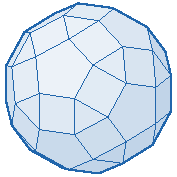
\includegraphics[width=26mm]{figures/rid}
\end{center}
\begin{abstract}
Can a solid pass through a straight tunnel drilled through an identical copy
of itself? Although it may seem counterintuitive, it turns out that a cube
can pass through itself in this way: John Wallis showed this in 1693,
settling a wager of Prince Rupert of the Rhine, after whom the property is
called \emph{Rupert's property}. All five Platonic solids turned out to share
it, and for a long time it seemed that every convex polyhedron might.
Passages were found for many highly regular solids, but some resisted
extensive randomised searches. Steininger and Yurkevich conjectured that the
rhombicosidodecahedron (RID), a highly regular Archimedean solid, does not
pass through itself, and a recent major result of theirs is a first
polyhedron without Rupert's property, the Noperthedron, constructed for the
purpose. We prove their conjecture for the RID using a computer-assisted
branch-and-bound elimination, which covers the entire symmetry-reduced
configuration space with $192{,}696$ regions, each verified with exact
arithmetic in $\mathbb Q(\sqrt5)$ to contain no passage. The RID is thereby
\textbf{the first Archimedean solid proved not to be Rupert}, and the first
such polyhedron that was not constructed for the purpose. Our main novel
addition is the \emph{zoom lemma}. The real obstacle is formed by the
configurations in which the two copies touch without either passing or
sticking out: no strict inequality holds there, so subdivision alone can
never eliminate their neighbourhoods. Near a set of configurations known to
contain no passage, the zoom lemma divides a necessary inequality exactly by
the distance from that set, so that one exact sign test eliminates a whole
neighbourhood, touching configurations included; the same lemma handles
every such case of the proof.
\end{abstract}
{\small\tableofcontents}

% !TEX root = ../main.tex
\pagebreak[0]
\section{Introduction}\label{sec:introduction}
\subsection{Rupert's property}\label{subsec:ruperts-property}

Can a cube pass through a hole in another cube of the same size?
The earliest known written account of this problem is by
\citet[pp.~470--471]{Wallis1693}, who records that Prince Rupert of the Rhine
wagered that it could. Wallis gave a geometric
solution to this apparently
impossible puzzle: suitably orienting the two cubes allows one to slide,
without turning, through a straight tunnel cut in the other, with positive
clearance. Thus the cube has \emph{Rupert's property}, or, equivalently,
the cube is \emph{Rupert}.
We call the moving body the \emph{plug} and the body through which it moves
the \emph{hole}.

It turns out that even a somewhat larger cube can pass through. The limiting
ratio of the plug's edge length to the hole's is
\[
  \frac{3\sqrt{2}}{4} \approx 1.060660172.
\]
The construction giving this ratio was found by Pieter Nieuwland and
published posthumously by \citet[pp.~608--610]{VanSwinden1816}.
Its optimality when the plug moves along a straight line without
turning was proved by
\citet{BezdekEtAl2021}. This limiting scale factor is called the cube's
\emph{Nieuwland number}; the same notion applies to other polyhedra.

\begin{figure}[htbp]
\centering
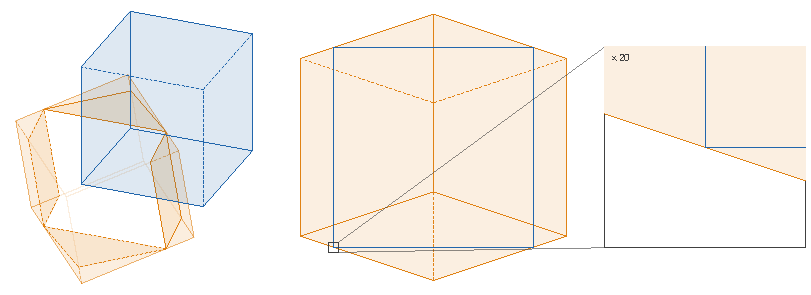
\includegraphics[width=0.85\linewidth]{figures/nieuwland-cube}
\caption{Nieuwland's passage for the cube. Left: \fc{Hole}{a unit cube (orange, faint)} with the tunnel cut out along the direction $(2,2,-1)$, and \fc{Plug}{a cube of edge $3\sqrt2/4$ (blue)} leaving it; only four wedges of the unit cube remain. Middle: both shadows along the direction of motion, a \fc{Plug}{square} inside a \fc{Hole}{hexagon}, \fc{Hole}{the hole's shadow tinted}. Right: a corner of the square, enlarged: it lies on the boundary of the hexagon, so no larger cube passes. In this and the later drawings, in space and in projection, the edges on the far side of each solid are dashed.}
\label{fig:nieuwland-cube}
\end{figure}

The same question applies to any convex polyhedron: can a congruent plug
pass through it in this way? \citet{JerrardWetzelYuan2017}
suggested that every convex polyhedron might be Rupert, and
\citet{ChaiYuanZamfirescu2018} stated this as a conjecture the following year.
A few years later, \citet{SteiningerYurkevich2023} conjectured that the
rhombicosidodecahedron (RID), a highly regular and symmetric Archimedean
solid with 60 vertices, was an exception. A polyhedron without Rupert's property is called \emph{Nopert}, a term
coined by Tom Murphy VII, also known as Tom~7, combining \emph{Nope} and
\emph{Rupert} \citep[p.~352]{Murphy2025}.
\citet{SteiningerYurkevichNopertV2} subsequently constructed the first convex polyhedron
proved to be Nopert, the \emph{Noperthedron}, but their proof did not settle
the RID \citep[Section~9.1]{SteiningerYurkevichNopertV2}.
Here we settle the RID's case with new geometric arguments that handle
its exotic cases.

\begin{theorem}\label{thm:main}
  The rhombicosidodecahedron is Nopert.
\end{theorem}

We call a choice of the plug's and hole's orientations, their relative displacement
and the direction of motion a \emph{configuration}.
The proof is computer-assisted. We divide the configuration space into
$192{,}696$ regions, each resolved using exact arithmetic calculations.
The final argument is given in
\cref{subsec:complete-coverage-and-the-main-theorem}.

\paragraph{The key idea.}
Most configurations are easy to rule out: some vertex of the plug sticks
out of the tunnel, and it still does after any small change of the
configuration, so a whole region around the configuration can be
eliminated at once. The obstacle is formed by the configurations in which
the plug touches the walls of the tunnel without sticking out. The
simplest example is a plug turned exactly like the hole: the two copies
then line up, and so do their shadows. Every strict inequality that could
exclude a fit vanishes at such a configuration, so no region containing
it can be eliminated by testing inequalities, however finely the regions
are subdivided. Yet the plug does stick out once it is turned slightly.
Suppose, for instance, that turning it by a small angle $x\ge0$ moves some
vertex outward by the amount $p(x,y)=x(1+x-y)$, where $y\in[0,1/2]$ stands
for the viewing direction. A sign test of $p$ must fail on any region
containing $x=0$, where $p$ vanishes. The factor $x$, however, is explicit:
the quotient $p/x=1+x-y$ is at least $1/2$ throughout, one sign test shows
it, and the configurations with $x=0$ are already known not to be fits.

We turn this observation into a single lemma, the \emph{zoom lemma}
(\cref{lem:zoom-lemma}). Around a set of configurations known to contain
no fit, a \emph{zoom} is a polynomial change of coordinates that
magnifies the neighbourhood of that set, so that the distance from it
becomes a coordinate that can be divided out exactly. After the division,
one exact sign test settles a whole region, including the touching
configurations themselves. The Local and Exotic components are instances of
this lemma, whose zooms differ only in the set around which they magnify
and in how many distances they divide out; the Domain and Global tests are
the same idea with nothing divided out. The four \emph{components} of the
proof, each a method for eliminating whole regions of configurations, are
listed in \cref{tab:components}.

\begin{table}[htbp]
\centering
\small
\begin{tabular}{llll}
  \toprule
  Component & Eliminates regions & Divides out & Section\\
  \midrule
  Domain & outside the symmetry-reduced domain & nothing & \ref{subsec:domain-component-skipping-boxes-outside-the-reduced-domain}\\
  Global & where some plug vertex sticks out & nothing & \ref{sec:global-component}\\
  Local & around the plug turned like the hole & the size of the rotation & \ref{sec:local-component}\\
  Exotic & around the other touching configurations & one or two distances & \ref{sec:square-and-pentagon-configurations}--\ref{sec:endpoint-and-crossing-configurations}\\
  \bottomrule
\end{tabular}
\caption{The four components of the proof.}
\label{tab:components}
\end{table}

\subsection{Previous approaches and the remaining difficulty}\label{subsec:previous-approaches-and-the-remaining-difficulty}

When the plug can pass through the hole with positive clearance, we call
this a \emph{fit} configuration.
To prove that a polyhedron is Rupert, even a single fit configuration is
enough, though finding one can be difficult. Examples include the
construction of \citet{Fredriksson2024} for the triakis tetrahedron and
the proof of \citet{RenshawRupertLean} in the Lean proof assistant that
Tom~7's candidate~\#214 is Rupert.
However, to prove that a polyhedron is Nopert, we must rule out every
possible fit configuration across the entire continuous space of
orientations, displacements and directions of motion. An unsuccessful
search over finitely many configurations, such as those sampled by the
randomized algorithms of \citet{SteiningerYurkevich2023}, however extensive,
is insufficient to rule out all infinitely many configurations.

\begin{figure}[htbp]
\centering
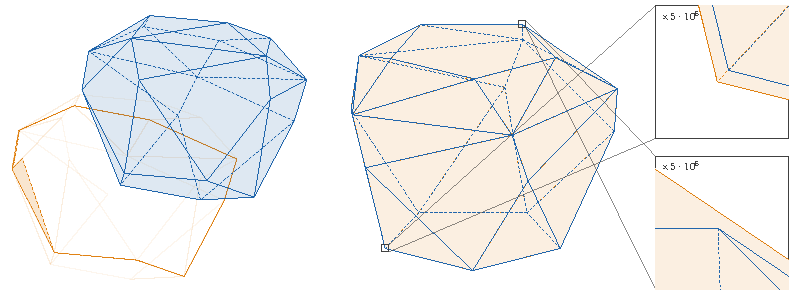
\includegraphics[width=0.85\linewidth]{figures/nopert214}
\caption{Tom~7's candidate~\#214 passes through itself, in the configuration of \citet{RenshawRupertLean}. Left: the tunnel removes all of \fc{Hole}{the hole (orange)} but a thin rim; \fc{Plug}{the plug (blue)} leaves it. Middle: the two shadows, indistinguishable at this scale. Right: the two places of least clearance, enlarged five million times; the gap is about $1.8\cdot10^{-8}$, for a solid of circumradius~$1$.}
\label{fig:nopert214}
\end{figure}

\paragraph{Constructive results and numerical searches.}
\citet{JerrardWetzelYuan2017} completed the proof that all five Platonic
solids are Rupert, building on earlier results for the cube, tetrahedron
and octahedron.
\begin{figure}[htbp]
\centering
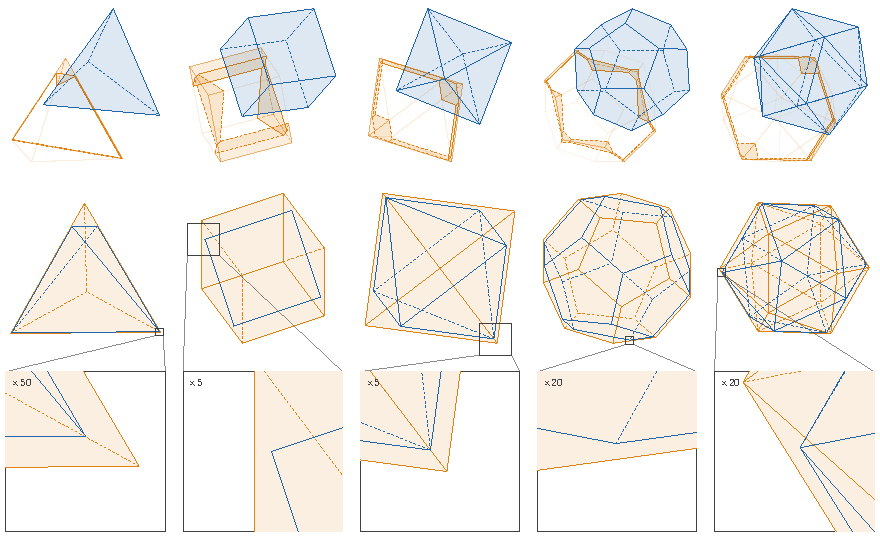
\includegraphics[width=0.95\linewidth]{figures/platonic}
\caption{Passages of the tetrahedron, cube, octahedron, dodecahedron and icosahedron, found by a numerical search. Top: \fc{Hole}{the hole (orange, faint)} with the tunnel cut out, and \fc{Plug}{the plug (blue)} leaving it. Middle: the shadows along the direction of motion. Bottom: the place of least clearance, enlarged. The plugs could be enlarged by factors of about $1.0145$, $1.0607$, $1.0607$, $1.0108$ and $1.0108$ and still pass; only the tetrahedron, which is not centrally symmetric, needs its plug's shadow shifted.}
\label{fig:platonic}
\end{figure}
\citet{ChaiYuanZamfirescu2018} examined the Archimedean solids and proved
Rupertness for eight of the thirteen. Subsequent work brought the total to
ten, leaving the snub cube, the RID and the snub dodecahedron unresolved
at that stage \citep{SteiningerYurkevich2023}.

Computational methods enabled more extensive searches for fit
configurations. \citet{SteiningerYurkevich2023} developed randomized searches
for such configurations and improved lower bounds for Nieuwland numbers
by perturbing known examples. \citet{Fredriksson2024} used nonlinear
optimization of the viewing directions from many starting points, and
\citet{GosainGrimmer2025V1} combined nonsmooth local optimization with
high-precision calculations of scale factors.

The triakis tetrahedron, a Catalan solid with eight vertices,
illustrates how a fit configuration can escape a large search.
It was among the solids left unresolved by \citet{SteiningerYurkevich2023}
in their randomized searches.
\citet{Fredriksson2024} then found a configuration giving a reported lower bound of
$1.000004$ for its Nieuwland number, corresponding to a clearance of only
about four parts per million in linear scale.
This shows how little room a fit configuration may have and gives
a concrete example of a configuration missed by earlier randomized searches.
More extensive searches and higher numerical precision can improve the
chances of finding such configurations, but failure to find one still does
not prove nonexistence.

\begin{figure}[htbp]
\centering
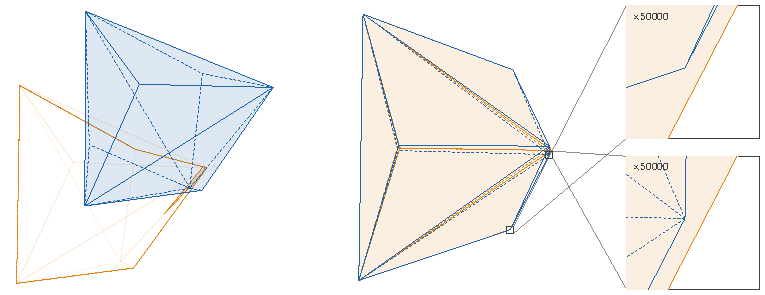
\includegraphics[width=0.82\linewidth]{figures/triakis}
\caption{The triakis tetrahedron passes through itself \citep{Fredriksson2024}. Drawn as in \cref{fig:nopert214}, with the two places of least clearance enlarged $50{,}000$ times; the gap is about $3.3\cdot10^{-6}$ at circumradius $5\sqrt6/8\approx1.53$. The parameters are Fredriksson's, refined slightly by a local numerical minimisation that changes none of them by more than $2.3\cdot10^{-5}$.}
\label{fig:triakis}
\end{figure}

\paragraph{Proving non-Rupertness.}
\citet{SteiningerYurkevichNopertV2} prove that the Noperthedron is Nopert
by combining arguments eliminating whole regions of configurations with
special treatment of boundary cases. They also explain why their local
theorem is insufficient for the RID, identifying an exotic viewing
direction and stating that its neighbourhood can be treated using
polynomial inequalities, while
reporting further difficult regions
\citep[Section~9.1]{SteiningerYurkevichNopertV2}.

The RID was a promising candidate for this research because of its highly
regular structure and many
symmetries, including central symmetry: reflecting it through its centre
leaves the RID unchanged. Central symmetry also simplifies the problem,
as explained in \cref{subsec:projection-containment}.
For such a regular solid, an extremely narrow, overlooked region of
fit configurations seemed less plausible to us. Despite this
intuition, we needed a way to recognise and rigorously verify a fit
configuration if one existed contrary to our expectations. We explain
how to handle this possibility in \cref{subsec:robustly-detecting-potential-rupertness}.

\citet{SteiningerYurkevich2023} also give an algorithm guaranteed to decide
whether a polyhedron with algebraic coordinates is Rupert, which they
describe as too computationally expensive for practical use.
Our aim is a feasible computer-assisted proof for the RID that addresses
the special configurations where ordinary elimination methods break down.

\subsection{Overview of the proof}\label{subsec:overview-of-the-proof}

For \emph{translative motion}, meaning motion without turning, the problem
has a useful two-dimensional description.
Project the plug and hole perpendicularly onto a plane normal to the direction
of motion, viewing their projections as filled \emph{shadows}. A fit configuration
is one in which the plug's shadow lies entirely in the interior of the hole's shadow.
For centrally symmetric convex bodies, relative translations can be removed:
if any relative displacement gives fit, coincident projected centres give
fit as well \citep{SteiningerYurkevich2023}. We give the argument in
\cref{subsec:projection-containment} so that this reduction requires no
background from the Rupert literature.

We may then fix the hole and describe a configuration by two parameters for
the viewing direction and three for the plug's relative rotation.
Our coordinates make the relevant expressions rational functions of these
five parameters. Clearing denominators of known positive sign reduces the
comparisons to polynomial inequalities. In contrast, the angular
parametrisation in the Noperthedron proof of
\citet[Section~6.1]{SteiningerYurkevichNopertV2} requires rigorously bounded
approximations to sine and cosine.
The RID's symmetries allow us to restrict attention to a small bounded
region of these coordinates while retaining at least one representative of
every remaining configuration. The parametrisation and the proof that these
representatives suffice are developed in
\cref{sec:geometric-formulation,sec:symmetry-reduced-domain}.

\paragraph{Eliminating configuration regions.}
Within that region, the procedure attempts to eliminate an entire parameter
region at once. Only representatives in the symmetry-reduced domain need to
be eliminated; regions entirely outside it can be skipped.
We call each method for certifying such an elimination a \emph{component}.
When no available component succeeds, the region is bisected
and both halves are retained for further examination. Failure of a test is
inconclusive: it neither establishes a fit configuration nor gives a reason
to discard the region. Together, the eliminated regions and their checked
reasons form a \emph{certificate}. \Cref{sec:branch-and-bound-elimination-in-the-reduced-domain}
explains the subdivision and what is required of such a certificate;
the exact calculations behind the checks are developed in
\cref{sec:reduction-to-exact-arithmetic}.

\paragraph{Completing the certificate.}
The remaining difficulty is to make subdivision terminate with a complete
certificate. We develop components successively to handle configurations
that the preceding ones leave unresolved.
First, if part of the plug's shadow protrudes beyond the hole's shadow,
we call this a \emph{poke} configuration. A sufficiently small change
preserves that protrusion, allowing us to eliminate a whole surrounding
region. The \emph{Global} component of \cref{sec:global-component}
eliminates these cases.

The difficulty arises when the plug's shadow is contained in the hole's,
but their boundaries meet: we call this a \emph{touch} configuration.
For example, in \emph{aligned configurations}, the plug and hole have the
same physical orientation, allowing for the RID's symmetries. The centred
bodies then coincide, as do their shadows. There is no protrusion to detect.
Further subdivision leaves at least one region containing the same touch
configuration, so testing for protrusion alone cannot complete the elimination.
We give formal definitions of fit, touch and poke in
\cref{subsec:the-margin-function-and-fit-poke-touch}.

Around aligned configurations, we instead study how the plug's vertices
move when the plug begins to rotate. The inequality expressing outward
motion contains the size of the rotation as an explicit factor, which
vanishes exactly at the aligned configurations, as in the example above.
\Cref{sec:local-component} develops the \emph{Local} component from this
observation and states the zoom lemma in general
(\cref{subsec:the-zoom-lemma}).
At two exotic viewing directions, the outward motion itself vanishes
to first order, and \cref{sec:square-and-pentagon-configurations} divides
out a second distance there.

Surprisingly, even after the aligned configurations have been
handled, non-aligned touch configurations remain---what
seems to us to be a rare feature of the RID\@. These families lie in two
planes of configurations that contain no fit, because in one direction the
plug reaches exactly as far as the hole. The same lemma, now dividing by
the distance from these planes, handles them, again with two distances at
the end of one family and where the two families cross
(\cref{sec:arc-configurations,sec:endpoint-and-crossing-configurations}).
These covers, together with those of
\cref{sec:square-and-pentagon-configurations}, form the \emph{Exotic}
component. With it, the collection of four components eliminates the
entire symmetry-reduced configuration space.

All accepted inequalities are checked with exact arithmetic. The final
certificate records a reason for each eliminated region. Its verification has
two distinct tasks: check that every reason is valid for all required
configurations in its region, and check that the regions together cover
all those configurations.
Together these establish \cref{thm:main}. We unify these requirements and
describe the implementation and computation details in
\cref{sec:generating-and-verifying-the-certificate}.

% !TEX root = ../main.tex
\pagebreak[0]
\section{Geometric formulation}\label{sec:geometric-formulation}
\subsection{The rhombicosidodecahedron}\label{subsec:the-rhombicosidodecahedron}

The RID is an Archimedean solid: all its faces are regular polygons---20
equilateral triangles, 30 squares and 12 regular pentagons---and it is
\emph{vertex-transitive}, meaning that its symmetries can carry any vertex
to any other. At each of its 60 vertices, the faces meet in the order
triangle, square, pentagon, square; altogether it has 120 edges
\citep{McCooeyRID}. It has icosahedral symmetry, which we will use to reduce
the configuration domain in \cref{sec:symmetry-reduced-domain}.

For the calculations, we need exact coordinates. The golden ratio
$\varphi=(1+\sqrt5)/2$, familiar from regular pentagons, makes these
particularly simple. Let $V$ consist of all
independent sign choices and cyclic coordinate permutations of
\begin{equation}\label{eq:rhombicosidodecahedron-vertices}
  (1,1,\varphi^3),\qquad
  (\varphi^2,\varphi,2\varphi),\qquad
  (2+\varphi,0,\varphi^2).
\end{equation}
Here cyclic permutation means replacing $(a,b,c)$ by $(b,c,a)$ or $(c,a,b)$.
The three families contain respectively 24, 24 and 12 distinct points,
giving the 60 vertices. Their convex hull, which we denote by $\mathcal R$, is the
filled RID with edge length two; these are also the coordinates used by
\citet{SteiningerYurkevich2023}.
Using edge length two keeps the coordinates simple. Rescaling both the plug
and hole by the same factor does not change whether they fit.

The sign choices make $V=-V$ and hence $\mathcal R=-\mathcal R$, expressing central symmetry
about the origin. The first family includes the eight corners of
$[-1,1]\times[-1,1]\times[-\varphi^3,\varphi^3]$, so the origin lies in
the interior of $\mathcal R$. This will let us compare the two shadows from a common
interior point.

The shape also appears outside polyhedral geometry: a modified RID forms
the connector balls in Zometool.\footnote{The author's childhood experience
of building with Zometool provided an additional motivation for choosing
the RID.} In the connector's idealized polyhedral model, the triangular
faces have edges $\varphi$ times as long as those of the pentagonal faces,
and rectangles with this same side ratio replace the squares
\citep[pp.~51, 197]{HartPicciotto2001}.

The golden ratio is present throughout this geometry: the 1,770 pairs of
vertices lie at 17 distinct distances, and all but two of their squares are
irrational numbers of the form $a+b\sqrt5$; the two exceptions are the
edge and the diagonal of a square face.

At unit edge length, the regular RID has volume
$(60+29\sqrt5)/3\approx41.6153$ \citep{McCooeyRID}, which rounds to 42.\footnote{Also
the answer to life, the universe and everything in \emph{The Hitchhiker's
Guide to the Galaxy} \citep{Adams1979}.}

\subsection{Projection containment}\label{subsec:projection-containment}

Fix a vector $\mathbf u\in\mathbb R^3\setminus\{\mathbf0\}$ along the direction
of motion. Orthogonal projection onto the plane $\mathbf u^\perp$ is the map
$\pi_{\mathbf u}:\mathbb R^3\to\mathbf u^\perp$ defined by
\[
  \pi_{\mathbf u}(\mathbf v)
    =\mathbf v-\frac{\mathbf v\cdot\mathbf u}{\mathbf u\cdot\mathbf u}\mathbf u.
\]
The image of a body under this map is its \emph{shadow}, including the
interior; the boundary of the shadow is its \emph{silhouette}. Since the
projection is linear, the shadow of $\mathcal R$ is the convex hull of the projected
vertices $\pi_{\mathbf u}(\mathbf v)$, for $\mathbf v\in V$.

Suppose initially that the hole is $R_{H}\mathcal R$ and the plug is $R_{P}\mathcal R+\mathbf a$, where
$R_{H},R_{P}\in\operatorname{SO}(3)$ are their rotations about the origin and
$\mathbf a\in\mathbb R^3$ is a displacement. Here $\operatorname{SO}(3)$ is
the group of real $3\times3$ orthogonal matrices with determinant $1$. Translating
the plug along $\mathbf u$ does not change its shadow. Over the whole line of motion,
the plug sweeps out the cylinder consisting of all lines parallel to $\mathbf u$ through
its shadow. The plug can pass through the hole with positive clearance,
giving a fit configuration, exactly when
\begin{equation}\label{eq:strict-projection-containment}
  \pi_{\mathbf u}(R_{P}\mathcal R)+\pi_{\mathbf u}(\mathbf a)
    \subseteq\operatorname{int}_{\mathbf u^\perp}\pi_{\mathbf u}(R_{H}\mathcal R),
\end{equation}
where the interior is taken in the two-dimensional screen plane
\citep[Proposition~1]{SteiningerYurkevich2023}.
Indeed, strict containment leaves room for a slightly wider cross-section
around the plug's shadow, still inside the hole's shadow, so the plug can
move through with positive clearance. Conversely, a fit requires the
entire plug shadow to lie in the interior of the hole shadow.
This is also called a \emph{strict fit}; without qualification, fit always
has this meaning.
A \emph{weak fit} requires only ordinary containment, allowing the plug's
shadow to meet the boundary of the hole's shadow. Such contact is permitted
but not required, so weak fit includes both fit and touch configurations.
Displacement along $\mathbf u$ only changes the plug's starting position, so only
the planar displacement $\pi_{\mathbf u}(\mathbf a)$ enters this comparison.

\paragraph{Removing translations.}
For centrally symmetric bodies, the planar displacement can be discarded.
The following short argument is the centering reduction of
\citet[Proposition~2]{SteiningerYurkevich2023}; it applies equally to weak fit
and to a uniformly scaled plug.

\begin{lemma}[Centering]\label{lem:centering}
  Let $P=-P$ and $H=-H$ be convex planar bodies centred at the origin.
  If a translate $P+\mathbf b$ is contained in $H$, then $P$ is contained in $H$.
  If $P+\mathbf b$ is contained in $\operatorname{int}H$, then $P$ is contained in
  $\operatorname{int}H$.
\end{lemma}
\begin{proof}
  Reflecting $P+\mathbf b\subseteq H$ through the origin gives $P-\mathbf b\subseteq H$.
  For each $\mathbf p\in P$, the points $\mathbf p+\mathbf b$ and $\mathbf p-\mathbf b$ belong to $H$, so their
  midpoint $\mathbf p$ belongs to $H$ by convexity. The same argument works in
  $\operatorname{int}H$, which is also convex and centrally symmetric.
\end{proof}

Both projected copies of $\mathcal R$ are centrally symmetric. Thus, for any fixed
orientations and viewing direction, a translated fit exists exactly when
the centred plug fits. Replacing $P$ by $\lambda P$ in
\cref{lem:centering} gives the same conclusion for each scale $\lambda>0$.
We may consequently restrict the search, and the optimization of scale, to
coincident projected centres. A displacement can still turn a fit configuration
into a touch or poke configuration; the reduction preserves the
existence of a fit.

\paragraph{Fixing the hole.}
Finally, rotating the whole configuration by $R_{H}^{-1}$ fixes the hole as $\mathcal R$
and replaces the plug rotation by $R_{H}^{-1}R_{P}$, with the viewing direction
rotated along with them. In this fixed-hole frame, we continue to write
$\mathbf u$ for the viewing vector and $R_{P}$ for the plug's rotation.
From now on, a configuration $c$ is centred and
consists of a viewing line together with the plug's rotation relative to
this fixed hole. The respective hole and plug shadows are:
\[
  H_c=\pi_{\mathbf u}(\mathcal R),\qquad P_c=\pi_{\mathbf u}(R_{P}\mathcal R).
\]
The sign and length of $\mathbf u$ do not matter: only its line matters. We are left
with two degrees of freedom for the viewing direction and three for the
relative rotation. For a polyhedron that is not centrally symmetric, the
component of the plug's displacement relative to the hole perpendicular
to the viewing direction must generally also be retained. This adds two
degrees of freedom, giving seven in total.

\subsection{Parametrisation of the configuration space}\label{subsec:parametrisation-of-the-configuration-space}

We choose coordinates that make the projected vertices rational functions
of five real parameters. This will allow us to compare their positions using
polynomial inequalities that we verify with exact arithmetic. We represent
the viewing line by a vector with positive $z$-coordinate, scaled to
\[
  \mathbf u=(s,t,1),\qquad (s,t)\in\mathbb R^2.
\]
Thus $s$ and $t$ determine the viewing line. The RID has sufficiently many symmetries
that we can choose such a representative with bounded $s,t$, without needing
any viewing direction in the $xy$-plane. We prove this reduction in
\cref{sec:symmetry-reduced-domain}.

\paragraph{Relative rotation.}
For the relative rotation, we use a nonzero quaternion
$q=(\alpha,\mathbf a)\ne(0,\mathbf0)$, consisting of a scalar part
$\alpha\in\mathbb R$ and a vector part $\mathbf a\in\mathbb R^3$.
We write $\lVert\cdot\rVert$ for Euclidean length.
A rotation by angle $\theta\in[0,\pi]$ around an axis
$\mathbf n\in\mathbb R^3$ with $\lVert\mathbf n\rVert=1$ is
represented by the unit quaternion
\[
  q=(\alpha,\mathbf a)=(\cos(\theta/2),\mathbf n\sin(\theta/2)).
\]
Here $\alpha^2+\lVert\mathbf a\rVert^2=1$. Nonzero real scalar multiples
represent the same rotation. Whenever $\alpha\ne0$, we may
therefore divide by it and write
\[
  q=(1,\mathbf r),\qquad
  \mathbf r=\frac{\mathbf a}{\alpha}=(r_1,r_2,r_3)\in\mathbb R^3.
\]
The vector $\mathbf r$ is a coordinate for the rotation, not the rotation
itself. For $\mathbf r\ne\mathbf 0$, its direction is the rotation axis and its
length is $\tan(\theta/2)$ for the angle $0<\theta<\pi$. The corresponding rotation
acts on a spatial vector $\mathbf v$ by
\begin{equation}\label{eq:relative-rotation}
  R_{P}(\mathbf r)\mathbf v
  =\frac{(1-\mathbf r\cdot\mathbf r)\mathbf v
      +2\mathbf r(\mathbf r\cdot\mathbf v)+2\mathbf r\times\mathbf v}
     {1+\mathbf r\cdot\mathbf r}.
\end{equation}
For example, the component parallel to $\mathbf r$ stays fixed; on the
perpendicular plane the two coefficients are
$(1-\lVert\mathbf r\rVert^2)/(1+\lVert\mathbf r\rVert^2)=\cos\theta$
and $2\lVert\mathbf r\rVert/(1+\lVert\mathbf r\rVert^2)=\sin\theta$.
This verifies the axis and angle and fixes the sign of the rotation.
At $\mathbf r=\mathbf 0$ the formula gives the identity matrix. In this
fixed-hole frame, a configuration is aligned exactly when the relative
rotation is a symmetry of $\mathcal R$.
We will denote a configuration by
$c=[s,t,\mathbf r]\in\mathbb R^2\times\mathbb R^3$, or equivalently
$[s,t,(r_1,r_2,r_3)]\in\mathbb R^5$, wherever these
coordinates are available.

\begin{figure}[htbp]
\centering
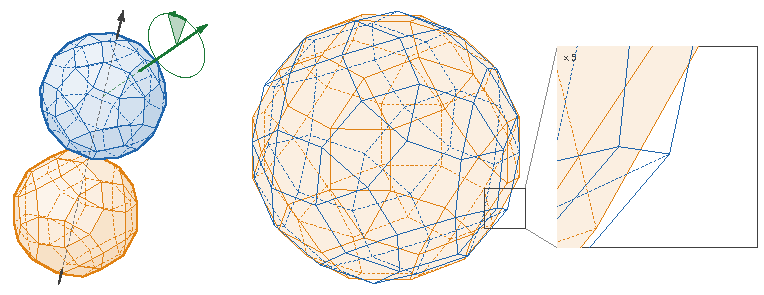
\includegraphics[width=0.78\linewidth]{figures/rid-parametrisation}
\caption{A configuration $c=[s,t,\mathbf r]$ with $s=1/5$, $t=1/10$ and $\mathbf r=(1/4,-1/12,5/24)$. Left: \fc{Hole}{the hole (orange)} and \fc{Plug}{the plug (blue)}, moved apart along the viewing direction $\mathbf u=(s,t,1)$ (black arrow) so that both can be seen. The plug is turned about \fc{Normal}{the axis $\mathbf n=\mathbf r/\lVert\mathbf r\rVert$ (green arrow, from the plug's centre) by the angle $\theta=2\arctan\lVert\mathbf r\rVert\approx37^\circ$, shaded on a circle about the axis}; dashed lines run behind or inside the solids. Middle: the two shadows along $\mathbf u$. Right: the plug's shadow sticks out of the hole's (enlarged five times), so this configuration is a poke.}
\label{fig:rid-parametrisation}
\end{figure}

\paragraph{Screen coordinates.}
There is a similarly simple choice of coordinates on the screen. Define
$L_{s,t}:\mathbb R^3\to\mathbb R^2$ by
\begin{equation}\label{eq:screen-map}
  L_{s,t}(v_1,v_2,v_3)=(v_1-sv_3,\ v_2-tv_3).
\end{equation}
Its kernel is precisely the viewing line spanned by $\mathbf u=(s,t,1)$.
Consequently, its restriction $T$ to $\mathbf u^\perp$ is an invertible linear map
from that plane to $\mathbb R^2$, and
$L_{s,t}=T\pi_{\mathbf u}$. In other words, it gives coordinates for the same
orthogonal shadow. Although these coordinates can distort lengths and
angles, applying the same invertible map to both shadows preserves
containment and containment in the interior. It also commutes with uniform
scaling, so every comparison of a scaled plug shadow with the hole shadow
is preserved.

Using these screen coordinates, we can write the hole and plug shadows as:
\begin{equation}\label{eq:shadow-coordinates}
  H_c=L_{s,t}\mathcal R
      =\operatorname{conv}\{L_{s,t}\mathbf v:\mathbf v\in V\},\qquad
  P_c=L_{s,t}R_{P}(\mathbf r)\mathcal R
      =\operatorname{conv}\{L_{s,t}R_{P}(\mathbf r)\mathbf v:\mathbf v\in V\}.
\end{equation}
Projected hole vertices have coordinates affine in $s,t$, while projected
plug vertices have rational coordinates with the common denominator
$d=1+\lVert\mathbf r\rVert^2\ge1$. Their coefficients belong to the quadratic field
\[
  \mathbb Q(\sqrt5)=\{a+b\sqrt5:a,b\in\mathbb Q\},
\]
because the vertices have coordinates in this field. Each coefficient is
represented exactly by the two rational numbers $a$ and $b$. Multiplying a
comparison by $d$, or by a positive power of $d$, preserves its sign.
This is how the rational expressions give polynomial inequalities without
requiring bounds on trigonometric or other transcendental functions.
The parameters themselves remain real;
the field describes the coefficients of these expressions.

This parametrisation does not represent rotations by $180^\circ$
(half-turns), whose representing quaternions have scalar part zero.
The reduction in \cref{sec:symmetry-reduced-domain} also provides bounded
relative-rotation representatives, including for these rotations.
Until that reduction is proved, a statement
about all configurations refers to the geometric configurations of
\cref{subsec:projection-containment}, not merely those represented by
these parameters.

\subsection{The margin function and \emph{fit} / \emph{poke} / \emph{touch}}\label{subsec:the-margin-function-and-fit-poke-touch}

To measure how close a configuration is to fitting, we compare the two
shadows on rays from their common origin. This gives a relative scale:
we ask how far the plug shadow extends compared with the hole shadow,
rather than measuring an absolute distance between their silhouettes.

For a compact convex shadow $C$ containing the origin in its interior and
a unit planar vector $\boldsymbol{\omega}$, define its \emph{radial extent} by
\[
  \rho_C(\boldsymbol{\omega})=\max\{\lambda\in\mathbb R_{\ge0}:\lambda\boldsymbol{\omega}\in C\}.
\]
Each ray meets $C$ in exactly the segment from the origin to
$\rho_C(\boldsymbol{\omega})\boldsymbol{\omega}$. This extent is positive and finite, and it varies
continuously with $\boldsymbol{\omega}$. To see the continuity, a limit of ray endpoints
still belongs to $C$, by compactness. In the other direction, any point
strictly between the origin and an endpoint is interior, by convexity and
the interior disk about zero; a small change of direction keeps that point
inside. Together these observations prevent either an upward or a downward
jump in radial extent.

\begin{definition}[Configuration margin]\label{def:configuration-margin}
  For a centred configuration $c$, with hole shadow $H_c$ and plug shadow
  $P_c$, define
  \begin{equation}\label{eq:configuration-margin}
    M_{\mathcal R}(c)=\max_{\lVert\boldsymbol{\omega}\rVert=1}
      \frac{\rho_{P_c}(\boldsymbol{\omega})}{\rho_{H_c}(\boldsymbol{\omega})}.
  \end{equation}
\end{definition}
The maximum exists because the unit circle is compact and the denominator
is positive. The largest ratio controls containment of the whole shadow:
it is the smallest factor by which the hole shadow must be scaled to
contain the plug shadow.

\begin{figure}[htbp]
\centering
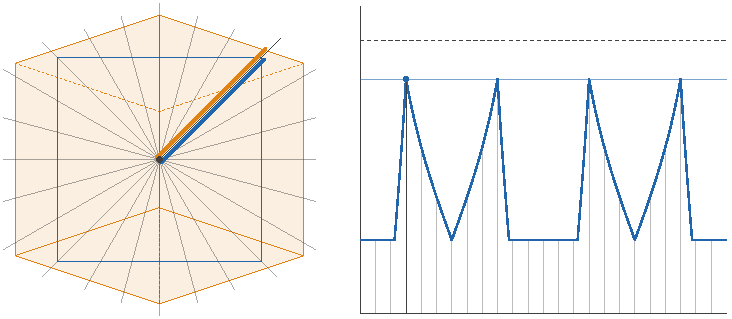
\includegraphics[width=0.78\linewidth]{figures/margin}
\caption{The margin of two congruent cubes $\mathcal C$ in the orientations of \cref{fig:nieuwland-cube}. Left: \fc{Hole}{the hole's shadow (orange)} and \fc{Plug}{the plug's (blue)} about their common centre, with rays every $15^\circ$; along the ray where the plug's radial extent is largest relative to the hole's, the two extents are drawn side by side. Right: that ratio over a full turn of directions, the \fc{Grey}{grey lines} marking the rays on the left. Its maximum, marked, is the margin $M_{\mathcal C}(c)=2\sqrt2/3\approx0.943$; it lies below the dashed level~$1$, so $c$ is a fit.}
\label{fig:margin}
\end{figure}

\begin{lemma}[Margin and containment]\label{lem:margin-and-containment}
  For every centred configuration $c$ and every $\lambda\in\mathbb R_{>0}$,
  \[
    P_c\subseteq\lambda H_c \quad\Longleftrightarrow\quad M_{\mathcal R}(c)\le\lambda,
    \qquad
    P_c\subseteq\operatorname{int}(\lambda H_c)
      \quad\Longleftrightarrow\quad M_{\mathcal R}(c)<\lambda.
  \]
  The margin is unchanged by applying the same invertible linear screen
  map to both shadows.
\end{lemma}
\begin{proof}
  Containment holds exactly when the plug shadow's radial extent is at most
  $\lambda$ times the hole shadow's in every direction. For interior
  containment, every radial comparison is strict. Since the maximum ratio
  is attained, these comparisons are equivalent to $M_{\mathcal R}(c)<\lambda$.
  Finally, an invertible linear map preserves each relation
  $P_c\subseteq\lambda H_c$, and hence preserves the least possible $\lambda$.
\end{proof}

In particular, the rational screen of \cref{eq:screen-map} gives the same
margin as orthogonal screen coordinates. We can now express the three
configuration types introduced in \cref{sec:introduction} as predicates:
\begin{equation}\label{eq:fit-poke-touch}
  \begin{aligned}
    \operatorname{fit}(c)   &\quad\Longleftrightarrow\quad M_{\mathcal R}(c)<1,\\
    \operatorname{touch}(c) &\quad\Longleftrightarrow\quad M_{\mathcal R}(c)=1,\\
    \operatorname{poke}(c)  &\quad\Longleftrightarrow\quad M_{\mathcal R}(c)>1.
  \end{aligned}
\end{equation}
A touch configuration has a weak fit with at least one boundary point shared by the two shadows. In the direction
from the common origin to such a point, the radial extents of the hole and
plug shadows match. In particular,
aligned configurations have identical shadows and margin one,
since their radial extents match for all $\boldsymbol{\omega}$.
Note that the silhouettes do not necessarily have to fully coincide in
a touch configuration.

\paragraph{Scale and the Nieuwland number.}
Scaling the plug by $\lambda>0$ multiplies every numerator in
\cref{eq:configuration-margin} by $\lambda$. It fits weakly exactly when
$\lambda M_{\mathcal R}(c)\le1$, and strictly exactly when $\lambda M_{\mathcal R}(c)<1$.
Thus $1/M_{\mathcal R}(c)$ is the maximum scale for weak fit and the supremum of the
scales for strict fit.

\emph{Optimising the margin over the full configuration space means taking
its infimum, which is the reciprocal of the Nieuwland number}
\citep[Definition~3]{SteiningerYurkevich2023}:
\begin{equation}\label{eq:nieuwland-number-and-margin}
  \nu(\mathcal R)=\sup_c\frac{1}{M_{\mathcal R}(c)}
        =\frac{1}{\inf_c M_{\mathcal R}(c)}.
\end{equation}
Here $c$ ranges over all centred geometric configurations. The centering
lemma shows that allowing translations does not improve this supremum.
It is finite: if $\mathcal R$ contains a ball of radius $a>0$ and is contained in
one of radius $b$, both centred at zero, then the orthogonal shadows contain
radius-$a$ disks and lie in radius-$b$ disks, giving
$a/b\le M_{\mathcal R}(c)\le b/a$. Aligned configurations give $\nu(\mathcal R)\ge1$.
Consequently \emph{$\mathcal R$ is Rupert exactly when $\nu(\mathcal R)>1$, and Nopert exactly
when $\nu(\mathcal R)=1$}. A barely Rupert body has a best margin just below one,
or equivalently a Nieuwland number just above one.

The examples in \cref{subsec:previous-approaches-and-the-remaining-difficulty}
show how little clearance known fit configurations can have. For the triakis
tetrahedron, \citet{Fredriksson2024} reported a lower bound of $1.000004$,
which \citet{GosainGrimmer2025V1} refined numerically to $1.000004055715$,
still only about four parts per million above one.
For Tom~7's candidate~\#214, the Lean formalisation of
\citet{RenshawRupertLean} proves fit,
and its accompanying source reports a shadow clearance of approximately
$1.8\times10^{-8}$ in the published coordinate units
\citep{Renshaw2026Nopert214Video,RenshawRupertLean}.
This last value measures a distance rather than a scale factor.

\paragraph{Continuity of the margin.}
After the compact
representative domain is established in \cref{sec:symmetry-reduced-domain},
continuity will also justify attaining the minimum margin there.

A useful geometric picture is that small changes to a configuration produce
small changes to its margin, even when the choice of projected vertices and
edges forming the silhouette changes discontinuously. For example, a projected
vertex can move onto or away from the boundary as the viewing direction
changes, while the shadow and its margin continue to vary continuously.

\begin{proposition}\label{prop:continuity-and-openness}
  The margin $M_{\mathcal R}$ is continuous on centred configurations. The sets of
  fit and poke configurations are open, and the set of touch configurations
  is closed.
\end{proposition}
\begin{proof}
  Work near any given configuration. Choose fixed spatial axes so that
  the viewing line has a representative with positive $z$-coordinate, and use the rational
  screen \cref{eq:screen-map} throughout a neighbourhood. Let the entries
  of the actual relative rotation matrix vary continuously; this includes
  half-turns. Each projected vertex then varies continuously, whether or
  not it lies on the silhouette.

  Compare configurations $c$ and $c'$, and let $\delta$ be the largest
  displacement between corresponding projected vertices of either body.
  Every point of a shadow is a convex combination of its projected
  vertices. Keeping the same coefficients in the other configuration gives
  a point within distance $\delta$, in both directions.
  All four shadows contain a common disk of some radius $a>0$ about zero:
  $\mathcal R$ and its rotations contain a radius-$a$ ball, and
  $L_{s,t}(v_1,v_2,0)=(v_1,v_2)$.

  Put $\lambda=1+\delta/a$. For any corresponding pair of shadows $C,C'$,
  the preceding distance bound implies $C\subseteq\lambda C'$.
  Indeed, write a point of $C$ as $\mathbf p+\mathbf z$, with $\mathbf p\in C'$ and
  $\lVert\mathbf z\rVert\le\delta$. If $\delta>0$, then
  \[
    \frac{\mathbf p+\mathbf z}{\lambda}
      =\frac{1}{\lambda}\mathbf p+
        \frac{\delta/a}{\lambda}\frac{a}{\delta}\mathbf z
      \in C'
  \]
  by convexity and the interior disk; if $\delta=0$, the inclusion is
  immediate. The reverse inclusion $C'\subseteq\lambda C$ follows in the
  same way. One factor of $\lambda$ compares the plug shadows and another
  compares the hole shadows:
  \[
    P_{c'}\subseteq\lambda P_c
      \subseteq\lambda M_{\mathcal R}(c)H_c
      \subseteq\lambda^2M_{\mathcal R}(c)H_{c'}.
  \]
  Using \cref{lem:margin-and-containment} and then reversing the roles of
  $c$ and $c'$ gives
  \[
    \lambda^{-2}M_{\mathcal R}(c)\le M_{\mathcal R}(c')\le\lambda^2M_{\mathcal R}(c).
  \]
  As $c'$ tends to $c$, the finitely many vertex displacements tend to
  zero, so $\lambda$ tends to one. This proves continuity. The openness
  and closedness statements follow from the comparisons with one in
  \cref{eq:fit-poke-touch}.
\end{proof}

% !TEX root = ../main.tex
\section{Symmetry-reduced domain}\label{sec:symmetry-reduced-domain}

The RID's symmetries introduce redundancy into the configuration space.
We can use this redundancy to restrict the parameter ranges for the viewing
direction and relative rotation to a small bounded region, while retaining
at least one representative of every configuration. This reduction also
justifies using the parametrisation of
\cref{subsec:parametrisation-of-the-configuration-space}: viewing directions
and relative rotations that it does not represent directly have equivalent
representatives within the chosen parameter ranges.

\subsection{Symmetries preserve the projection problem}\label{subsec:symmetries-preserve-the-projection-problem}

A \emph{body symmetry} is an orthogonal linear map taking $\mathcal R$ to itself.
Orientation-preserving body symmetries have determinant $1$ and are rotations;
orientation-reversing symmetries have determinant $-1$.
An orientation-reversing symmetry that fixes a plane pointwise is a
\emph{reflection}. Let $\mathcal G$ be the group of rotation symmetries.
Applying one of these to the plug before its
relative rotation does not change the plug at all: for $G_{P}\in\mathcal G$,
$R_{P}G_{P}\mathcal R=R_{P}\mathcal R$. Applying a hole symmetry $G_{H}\in\mathcal G$ to the whole
configuration also leaves the hole fixed as $\mathcal R$, while rotating the
viewing direction and plug together.

These two operations replace the viewing vector and relative rotation by
\[
  (\mathbf u,R_{P})\longmapsto(G_{H}\mathbf u,G_{H}R_{P}G_{P}),
  \qquad G_{H},G_{P}\in\mathcal G.
\]
Orthogonal projection respects this common change of frame:
\[
  \pi_{G_{H}\mathbf u}(G_{H}\mathbf v)=G_{H}\pi_{\mathbf u}(\mathbf v).
\]
Consequently, the two new shadows are the images of the old shadows under
the same planar isometry. Every containment comparison, including after
scaling either shadow by $\lambda>0$, is preserved. By
\cref{lem:margin-and-containment}, the margin is unchanged, as are the
truth values of the fit, touch and poke predicates.

We can also use the orientation-reversing symmetries. Since $\mathcal R=-\mathcal R$, any such
symmetry $G_{H}$ has $-G_{H}\in\mathcal G$.
Applying $-G_{H}$ instead keeps the plug's transformation a rotation, and its viewing
vector $-G_{H}\mathbf u$ represents the same line as $G_{H}\mathbf u$.
Thus all orthogonal body symmetries are available when choosing the
viewing line. They form $\mathcal G\cup(-\mathcal G)$.

Choosing the sign of the viewing vector also lets us make its $z$-coordinate
positive whenever it is nonzero, as assumed in the parametrisation of
\cref{subsec:parametrisation-of-the-configuration-space}. Viewing lines in
the $xy$-plane will be handled by the reduction in
\cref{subsec:rotation-and-reflection-reduction}.

\paragraph{The finite symmetry group.}
The RID has icosahedral symmetry, so $\mathcal G$ contains 60 rotations
and $-\mathcal G$ contains 60 orientation-reversing symmetries, including
15 planar reflections. Let $\mathcal Q$ be the set of unit quaternions representing
the rotations in $\mathcal G$, with both signs $g$ and $-g$ included for
each rotation. Thus $\mathcal Q$ has 120
members, whose coordinates belong to $\mathbb Q(\sqrt5)$. It includes all
eight signed coordinate-unit quaternions: one coordinate is $1$ or $-1$
and the other three are zero. The two signs represent the same rotation;
composing that rotation with central inversion gives its
orientation-reversing counterpart.
The quaternion families and exact checks establishing these finite facts
and the full symmetry count are given in
\cref{app:quaternion-families-and-the-full-symmetry-group}.

\subsection{Rotation and reflection reduction}\label{subsec:rotation-and-reflection-reduction}

We first restrict the viewing line, then keep its representative vector
$\mathbf u$ fixed while choosing the relative rotation. The reflection planes divide the viewing directions
into equivalent regions. We will select a representative in one closed
triangular region, including its boundary.

Reflections arise from the members of $\mathcal Q$ whose scalar part is zero. A unit quaternion
$(0,\mathbf n)$ represents the half-turn $2\mathbf n\mathbf n^{\mathsf T}-I$.
Its negative as a spatial matrix is the reflection
\[
  S_{\mathbf n}=I-2\mathbf n\mathbf n^{\mathsf T},
\]
which is a body symmetry by central inversion. There are 15 such normal
lines. Choose $\mathbf h=(1,2,9)$ and orient each unit normal so that
$\mathbf h\cdot\mathbf n>0$; none is perpendicular to $\mathbf h$.
This auxiliary vector chooses which side of each reflection plane we retain.

Among the images of a nonzero viewing vector under all 120 orthogonal symmetries,
choose one, still denoted by $\mathbf u$, that maximises
$\mathbf h\cdot\mathbf u$. If $\mathbf n\cdot\mathbf u<0$ for any of the
oriented normals, its reflection would give
\[
  \mathbf h\cdot(S_{\mathbf n}\mathbf u-\mathbf u)
    =-2(\mathbf h\cdot\mathbf n)(\mathbf n\cdot\mathbf u)>0,
\]
contradicting maximality. Thus the chosen vector $\mathbf u$ lies on the retained side
of every reflection plane.

\paragraph{The viewing triangle.}
Writing $\mathbf u=(u_1,u_2,u_3)$, the intersection of these 15 closed
halfspaces is exactly the cone
\begin{equation}\label{eq:viewing-cone}
  u_1\ge0,\qquad u_2\ge0,\qquad
  u_3\ge\varphi u_1+\varphi^2u_2.
\end{equation}
The equivalence between these halfspace conditions and the three cone
inequalities is proved in \cref{app:reflection-normals-and-the-viewing-cone}.

A nonzero vector in the cone has positive $z$-coordinate, so we can divide
by $u_3$ and write $\mathbf u=(s,t,1)$. The retained parameter pairs $(s,t)$
form the closed triangle
\begin{equation}\label{eq:viewing-triangle}
  s\ge0,\qquad t\ge0,\qquad \varphi s+\varphi^2t\le1.
\end{equation}
In particular, $s\le1/\varphi<2/3$ and $t\le1/\varphi^2<2/5$.
Every viewing line has a representative here, including lines initially
in the $xy$-plane. Ties in the maximisation cause no difficulty: we keep
all equality boundaries.

\paragraph{Choosing a rotation representative.}
For the relative rotation, the geometric aim is to choose an equivalent
description with as small a rotation angle as possible. Besides the plug's
symmetries, there is one more operation that preserves its shadow.
Let $J_{\mathbf u}$ be the half-turn about the viewing line. On the
perpendicular screen it changes every vector's sign, so
\[
  \pi_{\mathbf u}J_{\mathbf u}=-\pi_{\mathbf u}.
\]
The plug is centrally symmetric, and consequently
\begin{equation}\label{eq:projected-half-turn}
  \pi_{\mathbf u}J_{\mathbf u}R_{P}\mathcal R
    =-\pi_{\mathbf u}R_{P}\mathcal R
    =\pi_{\mathbf u}R_{P}\mathcal R.
\end{equation}
We may therefore apply this half-turn to the plug while keeping the hole
and viewing vector $\mathbf u$ fixed. It need not be a symmetry of the plug: it preserves the plug's
shadow, which is what the containment comparison uses.

Quaternion multiplication expresses both operations simply. With scalar
parts $\alpha,\beta\in\mathbb R$ and vector parts
$\mathbf a,\mathbf b\in\mathbb R^3$, its convention is
\begin{equation}\label{eq:quaternion-product}
  (\alpha,\mathbf a)(\beta,\mathbf b)
    =(\alpha\beta-\mathbf a\cdot\mathbf b,\;
      \alpha\mathbf b+\beta\mathbf a+\mathbf a\times\mathbf b).
\end{equation}
The product represents composition in the same order as rotation
matrices: the right-hand rotation acts first. Since $\mathcal G$ is closed
under composition and both quaternion signs are included, $\mathcal Q$ is
closed under this product. Let $p$ be a unit quaternion of the
current relative rotation, and put
\[
  j=\frac{(0,\mathbf u)}{\lVert\mathbf u\rVert},\qquad
  \lVert\mathbf u\rVert^2=1+s^2+t^2.
\]
Then $j$ represents $J_{\mathbf u}$ and $j^2=-1$.

We choose a quaternion $p_*$ with largest scalar part from the finite set
\begin{equation}\label{eq:rotation-representative-family}
  \{p g,\ j p g:g\in\mathcal Q\}.
\end{equation}
Both quaternion signs occur. For a unit quaternion with nonnegative
scalar part, that part is $\cos(\theta/2)$ for $0\le\theta\le\pi$.
Maximising it therefore minimises the relative rotation angle among
these equivalent descriptions.
The set in \cref{eq:rotation-representative-family} is unchanged by
further right multiplication by a member of $\mathcal Q$, or by left
multiplication by $j$: closure of $\mathcal Q$ gives the first assertion,
and $j^2=-1$, together with both signs, gives the second.
Thus the chosen representative satisfies both sets of comparisons
simultaneously.

Write $p_*=(\alpha,\mathbf a)$. Its scalar part
$\alpha=\operatorname{scalar}(p_*)$ is at least $1/2$.
Indeed, the signed coordinate-unit quaternions in $\mathcal Q$ can move
any chosen coordinate of $p$, with either sign, to the scalar position.
At least one of the four coordinates of a unit quaternion has absolute
value at least $1/2$. We can therefore divide by $\alpha>0$ to obtain
\[
  p_*=\alpha(1,\mathbf r),\qquad
  \mathbf r=\frac{\mathbf a}{\alpha}.
\]
This gives a representative even when the original relative rotation
was a half-turn, represented by a quaternion with scalar part zero.

\paragraph{Bounds from body symmetries.}
The comparisons with plug symmetries acting on the right give
$\operatorname{scalar}((1,\mathbf r)g)\le1$ for every $g\in\mathcal Q$.
Use cyclic subscripts, with $r_4=r_1$.
Twelve particular group elements give the comparisons
\begin{equation}\label{eq:rotation-comparisons}
  \epsilon r_i+(-1+\varphi)\delta r_{i+1}\le2-\varphi,
  \qquad i=1,2,3,\quad \epsilon,\delta\in\{-1,1\}.
\end{equation}
These group elements and their substitutions are given in
\cref{app:selected-quaternions-for-the-rotation-comparisons}.
Averaging the two inequalities with opposite signs of $\delta$ gives
$\epsilon r_i\le2-\varphi$. Using both signs of $\epsilon$, we obtain
$|r_i|\le2-\varphi<2/5$. These necessary comparisons provide the
bounded rotation coordinates we need; we do not need to characterise
all scalar-maximising representatives.

\paragraph{The fold inequalities.}
The comparisons involving the projected half-turn, which we call the
\emph{fold}, yield further restrictions; the next paragraph explains why
they are needed. Since both $g$ and $-g$ are available, maximality gives
$|\operatorname{scalar}(j p_*g)|\le\alpha$. Define
\begin{equation}\label{eq:fold-polynomial}
  \ell_g(c)=\operatorname{scalar}\bigl((0,\mathbf u)(1,\mathbf r)g\bigr).
\end{equation}
Substituting $p_*=\alpha(1,\mathbf r)$ and cancelling $\alpha>0$ gives
$|\ell_g(c)|\le\lVert\mathbf u\rVert$, or equivalently
\begin{equation}\label{eq:fold-comparisons}
  {\ell_g(c)}^2\le1+s^2+t^2.
\end{equation}
Squaring loses no sign information because the preceding comparison is
two-sided. Opposite quaternions give the same squared inequality, leaving
60 inequalities. Let $\mathcal Q_+$ contain one quaternion from each pair
$g,-g$, choosing the one whose first nonzero coordinate is positive.
It suffices to impose \cref{eq:fold-comparisons} for $g\in\mathcal Q_+$.
If $g=(\beta,\mathbf b)$, the product formula gives
\[
  \ell_g(c)=-\beta\mathbf u\cdot\mathbf r
           -\mathbf b\cdot(\mathbf u+\mathbf u\times\mathbf r).
\]
Thus these are polynomial inequalities in our five parameters, with
coefficients in $\mathbb Q(\sqrt5)$.

\paragraph{A second family with equal shadows.}
The fold matters near aligned configurations. The aligned configurations
$\mathbf r=\mathbf0$ have exactly the hole's shadow, and so does a second
family. Let $Z$ be the half-turn symmetry
about the $z$-axis applied to the plug, represented by $k=(0,0,0,1)$.
Since $Z\mathcal R=\mathcal R$, the plug $J_{\mathbf u}Z\mathcal R$ has exactly the hole's shadow by
\cref{eq:projected-half-turn}. The product
\begin{equation}\label{eq:equal-shadow-rotation}
  -jk=\frac{(1,-t,s,0)}{\lVert\mathbf u\rVert}
\end{equation}
shows that this family has rotation coordinates $\mathbf r=(-t,s,0)$.
Its touch configurations approach $\mathbf r=\mathbf0$ as $(s,t)$
approaches $(0,0)$. For $g=k$, the fold inequality is
\[
  {(1+sr_2-tr_1)}^2\le1+s^2+t^2.
\]
On this family it simplifies to $\lVert\mathbf u\rVert\le1$, which holds
only at $s=t=0$.
The fold removes the other representatives of this family; their identical
shadows already have representatives with $\mathbf r=\mathbf0$ at the
same parameter pair $(s,t)$. This separation will be useful when proving the local results
around aligned configurations.

\subsection{The reduced domain}\label{subsec:the-reduced-domain}

The preceding bounds place a representative of every configuration in the
five-dimensional rectangle
\begin{equation}\label{eq:search-rectangle}
  B_0=\left[0,\frac23\right]\times\left[0,\frac25\right]
       \times{\left[-\frac25,\frac25\right]}^3.
\end{equation}
The first two intervals describe $s,t$ and the last three describe
$\mathbf r=(r_1,r_2,r_3)$. Within this rectangle, define the reduced domain
\begin{equation}\label{eq:reduced-domain}
  D=\left\{c=[s,t,\mathbf r]\in B_0:
  \begin{aligned}
    \varphi s+\varphi^2t&\le1,\\
    \epsilon r_i+(-1+\varphi)\delta r_{i+1}&\le2-\varphi
      &&(i=1,2,3;\ \epsilon,\delta\in\{-1,1\}),\\
    {\ell_g(c)}^2&\le1+s^2+t^2 &&(g\in\mathcal Q_+)
  \end{aligned}\right\}.
\end{equation}
These are the viewing-triangle condition, twelve relative-rotation
comparisons and sixty fold comparisons: 73 inequalities in total, in
addition to the interval bounds defining $B_0$.

\begin{figure}[htbp]
\centering
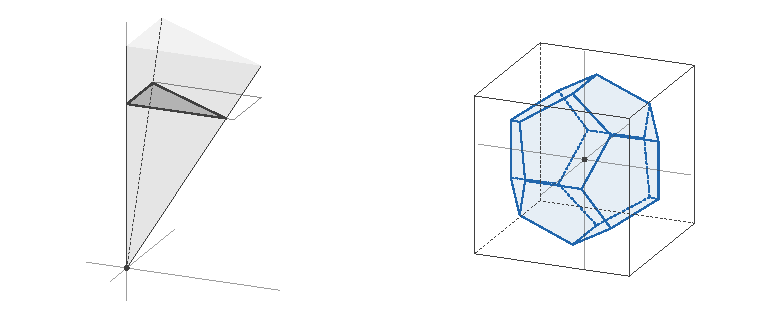
\includegraphics[width=0.82\linewidth]{figures/reduced-ranges}
\caption{The reduced ranges, in the spatial axes of \cref{fig:rid-parametrisation}. Left: the viewing directions kept form a \fc{Grey}{cone (grey)} through the viewing triangle $s,t\ge0$, $\varphi s+\varphi^2t\le1$ in the plane $z=1$ (dark), which lies in the rectangle $[0,2/3]\times[0,2/5]$ of $B_0$ (thin). Right: the box ${[-2/5,2/5]}^3$ of rotation vectors $\mathbf r$ (grey) and the part of it satisfying the twelve rotation comparisons \fc{Plug}{(blue), a dodecahedron}; the fold comparisons, which also involve $s$ and $t$, cut it further.}
\label{fig:reduced-ranges}
\end{figure}

\begin{proposition}[Representative coverage]\label{prop:representative-coverage}
  Every centred geometric configuration has a representative in $D$ with
  the same margin. In particular, a fit exists if and only if one
  exists in $D$.
\end{proposition}
\begin{proof}
  First apply a hole symmetry to the viewing line and the common frame
  to place the representative vector $\mathbf u$ in the cone
  \cref{eq:viewing-cone}. An orientation-reversing
  symmetry is implemented by its negative, with the viewing vector's sign
  reversed, as in \cref{subsec:symmetries-preserve-the-projection-problem}.
  The transformed vector has positive $z$-coordinate, so normalising it gives
  $\mathbf u=(s,t,1)$ satisfying \cref{eq:viewing-triangle} and the first
  two interval bounds of $B_0$.

  Keep $(s,t)$ fixed and choose the maximal-scalar quaternion from
  \cref{eq:rotation-representative-family}. Its positive scalar part
  permits the normalisation $(1,\mathbf r)$, and its comparisons give
  \cref{eq:rotation-comparisons,eq:fold-comparisons} and the remaining
  interval bounds of $B_0$. Every operation preserves the margin, so
  this is the required representative. Conversely, each point of $D$
  specifies an actual viewing line and rotation by the formulas of
  \cref{subsec:parametrisation-of-the-configuration-space}.
\end{proof}

All the inequalities are non-strict. In particular, the argument retains
viewing directions lying in reflection planes, ties between rotation representatives and
equality in the fold comparisons. A configuration can have more than one
representative in $D$; coverage is all that the proof needs.
For a configuration initially allowing displacement, the centering lemma
first preserves the existence of a fit, and the proposition then
puts a centred fit in $D$.

\paragraph{Compactness and the minimum margin.}
The coverage proposition ensures that $D$ is nonempty. Its polynomial
inequalities define a closed subset of the compact rectangle $B_0$,
so $D$ is compact. By \cref{prop:continuity-and-openness}, the margin
therefore attains its minimum on $D$. Representative coverage gives the promised bounded
form of \cref{eq:nieuwland-number-and-margin}:
\begin{equation}\label{eq:nieuwland-number-on-reduced-domain}
  \nu(\mathcal R)=\frac{1}{\displaystyle\min_{c\in D}M_{\mathcal R}(c)}.
\end{equation}
The remaining task is to show that $M_{\mathcal R}(c)\ge1$ throughout $D$.
We will work from the simpler enclosing rectangle $B_0$ and use these
inequalities to set aside regions entirely outside $D$. Their physical
configurations already have representatives in $D$; no classification of these
as fit, touch or poke configurations is needed to set those regions aside.

% !TEX root = ../main.tex
\section{Branch and bound elimination in the reduced domain}\label{sec:branch-and-bound-elimination-in-the-reduced-domain}

To rule out fit throughout $D$, we examine whole regions of configurations
at a time. Each successful component must rule out fit for every configuration in
the region that belongs to $D$. We subdivide unresolved regions, seeking a
resolution high enough for at least one component to eliminate them.
The proof rests on two facts about the result: every region was eliminated
soundly, and the eliminated regions cover $D$.
\Cref{sec:generating-and-verifying-the-certificate} checks both for the
final certificate and lists everything the proof relies on. The notions of
range and completion in \cref{subsec:component-hierarchy} explain why the
subdivision finishes and how the components were found; the proof itself
does not use them.

\subsection{Boxes, subdivision, and elimination}\label{subsec:boxes-subdivision-and-elimination}

A \emph{box} is a Cartesian product of closed parameter intervals,
\[
  B=\prod_{i=1}^{5}[l_i,h_i]\subseteq B_0,
  \qquad l_i,h_i\in\mathbb Q,\quad l_i\le h_i,
\]
in the coordinate order $s,t,r_1,r_2,r_3$. Each point of $B$ represents a
configuration. Rational endpoints allow the box itself
to be recorded exactly. The boxes created by our search have positive
width in every coordinate, so they cover entire five-dimensional regions
of configuration space.

We \emph{eliminate} a box when we certify that it contains no fit
configuration in $D$. In terms of the margin, the required conclusion is
\begin{equation}\label{eq:box-elimination}
  M_{\mathcal R}(c)\ge1\qquad\text{for all }c\in B\cap D.
\end{equation}
A component takes a box and attempts to justify its elimination. If it
succeeds, we store a \emph{certificate record} identifying the box, the
successful component and the data needed to verify its result. Otherwise,
its answer is inconclusive.
A component is \emph{sound} if every accepted result establishes
\cref{eq:box-elimination}.
In particular, elimination allows touch configurations, and a box disjoint
from $D$ satisfies this condition without any geometric comparison.

\paragraph{Subdivision.}
We call a set of components used together for elimination a \emph{collection}.
The procedure starts with $B_0$. For each unresolved box, it tries the
members of the collection in a fixed order, stopping at the first successful one. If none
succeeds, it bisects one of the intervals at its midpoint
$m=(l_i+h_i)/2$, replacing $[l_i,h_i]$ by $[l_i,m]$ and $[m,h_i]$ while
leaving the other four intervals unchanged. Both children are closed,
axis-parallel boxes containing the four-dimensional dividing face, and
their union is exactly the parent box.

The number of bisections from $B_0$ to a box is its \emph{depth}. We bisect
coordinates cyclically in the order $s,t,r_1,r_2,r_3$, and process boxes in
increasing depth. Boxes that remain unresolved are therefore refined adaptively
to arbitrarily small widths in all five coordinates. The decision to subdivide depends on
whether a box has been eliminated; the coordinate order does not.

\paragraph{Complete coverage.}
An important invariant is that the eliminated boxes together with the unresolved
boxes always cover $B_0$. This holds initially and is preserved both when a box is
eliminated and when it is replaced by its two children. Consequently, if
the procedure finishes with finitely many eliminated boxes and none
unresolved, their certificate records form a complete certificate of
non-Rupertness. Indeed, a fit would have a representative in $D$
by \cref{prop:representative-coverage}. That representative would belong
to an eliminated box, contradicting \cref{eq:box-elimination}. Shared
boundaries introduced by the bisections cause no exception to this reasoning.

This explains what completion would prove; it does not yet show that the
collection will resolve every box. Stopping at a time or depth limit leaves
the unresolved regions to be treated. \Cref{sec:generating-and-verifying-the-certificate}
describes how these records and their coverage are checked.

For convex polyhedra with algebraic vertex coordinates,
\citet{SteiningerYurkevich2023} give the theoretical decision procedure
discussed in \cref{subsec:previous-approaches-and-the-remaining-difficulty}.
Their procedure reduces
the problem to solving systems of polynomial equations and inequalities,
but they regard the resulting computations as impractical. Our aim is to
develop a collection that uses the geometric properties of the RID
to make certificate generation feasible.

\subsection{Component hierarchy}\label{subsec:component-hierarchy}

Even though components are applied to entire boxes, their usefulness and
scope can be better understood by considering individual configurations.
If a component works uniformly throughout some neighbourhood
around a configuration, it will generally handle sufficiently small boxes
there. We make this connection precise so that later descriptions of where
a component applies have a common and unambiguous meaning.

Call any box obtainable by the cyclic midpoint subdivision of $B_0$ a
\emph{search box}, whether or not a particular run reaches it. Neighbourhoods
below are relative to $B_0$: at its boundary, only configurations inside
$B_0$ need to be considered. Distances and diameters refer to Euclidean
distance between the five parameter coordinates.

\begin{lemma}[Search boxes in neighbourhoods]\label{lem:search-boxes-in-neighbourhoods}
  Every configuration $c\in B_0$ belongs to a search box at every depth.
  For any neighbourhood $U$ of $c$ relative to $B_0$, all sufficiently deep
  search boxes containing $c$ lie entirely in $U$. In particular, every
  nonempty relatively open subset of $B_0$ contains a search box.
\end{lemma}
\begin{proof}
  The full subdivision at each depth covers $B_0$, since the two closed
  children cover their parent. At depth $d$, each coordinate has been
  bisected at least $\lfloor d/5\rfloor$ times, so every search box at that
  depth satisfies
  \begin{equation}\label{eq:search-box-diameter-bound}
    \operatorname{diam}B
      \le 2^{-\lfloor d/5\rfloor}\operatorname{diam}B_0.
  \end{equation}
  Choose $\varepsilon>0$ such that every point of $B_0$ at distance less
  than $\varepsilon$ from $c$ belongs to $U$. For sufficiently large $d$,
  this diameter bound is less than $\varepsilon$, so every point of a
  search box containing $c$ belongs to $U$. The argument also applies
  when $c$ lies on a boundary of $B_0$ or a subdivision face.
\end{proof}

\begin{definition}[Range of a component]\label{def:range-of-a-component}
  A configuration $c\in B_0$ belongs to the \emph{range} of a component if
  it has a neighbourhood $U$ in $B_0$ such that the component accepts every
  search box $B\subseteq U$. The range of a collection is
  defined in the same way, allowing any member to accept
  each such box.
\end{definition}

Acceptance here means that the component's check succeeds, including any
selection of the data needed for its certificate record. A box does not count
as accepted just because a valid record exists; the component must find and
verify one. Different boxes may use different data in their records, or
different members of a collection. This definition describes an open region
relative to $B_0$.

In particular, accepting one closed box with $c$ on its boundary does not
establish that $c$ lies in the component's range. Smaller boxes around $c$
can extend across that boundary. The same issue arises where two proved
regions meet: a box extending across both regions needs a component that can
certify all of it. A component may check that the box is covered by a union of already
proved regions, or another component may handle the whole box. Acceptance
of only the box's centre is not enough.

\begin{lemma}[Finite completion from local coverage]\label{lem:finite-completion-from-local-coverage}
  Suppose the range of a fixed finite collection covers $B_0$, all its
  members are sound, and every component call finishes. Then the increasing-depth search
  with cyclic midpoint subdivision terminates after finitely many boxes,
  provided no time or depth limit stops it.
\end{lemma}
\begin{proof}
  Around each configuration in $B_0$, choose a ball of radius $2\varepsilon$, with
  $\varepsilon>0$, whose intersection with $B_0$ lies in an accepting
  neighbourhood. The balls with radii $\varepsilon$ still cover $B_0$.
  Compactness gives a finite subcover; let $\delta>0$ be the smallest
  radius in that finite subcover.

  Any search box of diameter less than $\delta$ lies in one of the
  corresponding larger balls. Indeed, choose a point of the box and a
  smaller ball containing it. Every other point of the box is within
  $\delta$ of that point, hence within twice the smaller ball's radius
  of its centre. Such a box is therefore accepted.

  By \cref{eq:search-box-diameter-bound}, at sufficiently large finite
  depth every search box has diameter less than $\delta$, so every box
  at that depth is accepted without further subdivision.
  There are only finitely many boxes up to that depth, and processing each
  one takes finitely many component calls, all of which finish. The search
  therefore terminates.
\end{proof}

\paragraph{Developing the collection.}
The same finite-cover reasoning applies to any compact subset of the
collection's range: sufficiently small unresolved boxes cannot continue
to meet that subset. Refinement can therefore help locate the configurations
for which further components are needed. Small changes in the margin alone
do not establish this property; we must show that the relevant component
actually succeeds on the nearby boxes.

This gives a way to develop the collection successively. When refinement
concentrates on configurations the current collection cannot handle, we
examine their geometry and add a component to handle them. Each addition works
alongside the preceding components. The need to treat aligned configurations
was already apparent before running the Global component, which detects
protrusion: at an aligned configuration the shadows coincide, so no
projected plug vertex protrudes beyond the hole's shadow.

The final collection has four components, in the order in which we develop
them: the \emph{Domain} component (\cref{subsec:domain-component-skipping-boxes-outside-the-reduced-domain}),
which discards boxes outside $D$; the \emph{Global} component
(\cref{sec:global-component}), for poke configurations; the \emph{Local}
component (\cref{sec:local-component}), for neighbourhoods of aligned
configurations; and the \emph{Exotic} component
(\cref{sec:square-and-pentagon-configurations,sec:arc-configurations,sec:endpoint-and-crossing-configurations}),
with eight covers around the remaining touch configurations.
\Cref{fig:hierarchy} shows how each addition clears boxes that the
preceding components leave unresolved. The program may try an inexpensive
specialised check before a more general one; the order affects only which
record a box receives.

\begin{figure}[htbp]
\centering
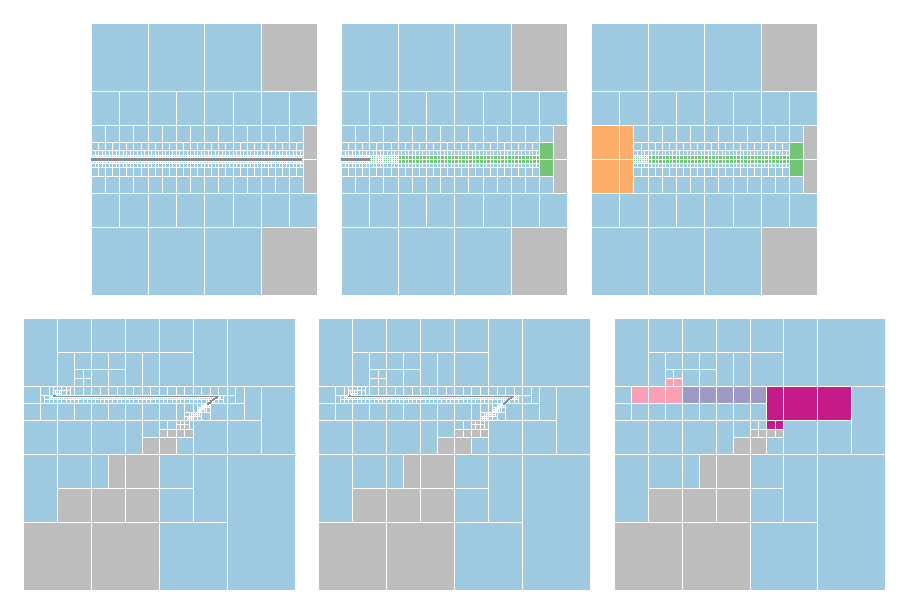
\includegraphics[width=\linewidth]{figures/hierarchy}
\caption{The collection built up component by component on two planes of configurations, each halved alternately until a component eliminates a piece or the piece is $16$ (top) or $18$ (bottom) halvings deep; pieces still unresolved at that depth are black. Top: the plane $t=0$, $r_1=r_2=0$ through the square configuration, with $s\in[0,2/3]$ horizontally and $r_3\in[-2/5,2/5]$ vertically. Bottom: the plane $\Pi_1$ of \cref{sec:arc-configurations}, with $s\in[3/16,5/8]$ horizontally and $\theta\in[-5/16,1/8]$ vertically. Left: the \fc{Domain}{Domain (grey)} and \fc{Global}{Global (light blue)} components leave the aligned configurations $r_3=0$ and the two arcs unresolved. Middle: the \fc{Local}{Local component (green)} eliminates the aligned configurations except near the square configuration $s=0$, and nothing on the arcs. Right: the whole collection, which leaves nothing; the Exotic covers (\fc{Square}{square light orange}, \fc{Arc}{arc lavender}, \fc{Endpoint}{endpoint light pink}, \fc{Crossing}{crossing magenta}) are tried before the Local component, so the square cover also takes pieces that the Local component would eliminate.}
\label{fig:hierarchy}
\end{figure}

\subsection{\emph{Domain} component: skipping boxes outside the reduced domain}\label{subsec:domain-component-skipping-boxes-outside-the-reduced-domain}

The simplest component uses the inequalities defining $D$ in
\cref{eq:reduced-domain}. If one of them is strictly violated throughout
$B$, then $B\cap D=\varnothing$. We call this the \emph{Domain} component.
The justification is the representative-coverage result: the configurations
discarded here already have representatives in $D$. They need not be poke configurations.

\paragraph{Affine inequalities.}
The viewing-triangle inequality and the twelve relative-rotation inequalities
are affine. Write one as $p(c)\le0$, subtracting its right side from its
left side. To minimise $p$ on $B$, choose the lower endpoint in every
coordinate with a positive coefficient and the upper endpoint for a negative
coefficient; a zero coefficient permits either choice. This gives the exact
minimum. If it is strictly positive, the entire box violates the inequality.
Equality is insufficient because the inequalities defining $D$ are
non-strict.

\paragraph{Fold inequalities.}
The fold inequalities require more care. A \emph{corner} of a box is
obtained by choosing an endpoint of each parameter interval. We group
these choices according to what they control. The allowed pairs $(s,t)$
fill a rectangle in the $(s,t)$-plane, which we call the \emph{viewing
rectangle}. Choosing an endpoint for each of $s$ and $t$ gives its four
corners, each specifying a viewing direction. Independently, the allowed
vectors $\mathbf r=(r_1,r_2,r_3)$ fill a three-dimensional \emph{rotation box},
whose eight corners choose an endpoint for each of $r_1,r_2,r_3$. Each viewing
corner can be combined with any rotation corner, giving the $4\times8=32$
corner configurations of $B$.

The square of an expression can be large at both ends of an
interval while the expression changes sign and vanishes inside. For this
reason, evaluating only the squared fold inequalities at the corners would
not justify eliminating the box. We also check the sign before squaring.

\begin{proposition}[Whole-box fold violation]\label{prop:whole-box-fold-violation}
  Fix $g\in\mathcal Q_+$. The inequality
  \[
    {\ell_g(c)}^2>1+s^2+t^2
  \]
  holds throughout $B$ if and only if it holds at every corner of $B$
  and the values of $\ell_g$ at all corners have one common nonzero sign.
\end{proposition}
\begin{proof}
  Suppose first that the corner conditions hold, and let
  $\sigma\in\{-1,1\}$ be the common sign. At every corner,
  \[
    \sigma\ell_g(c)-\lVert\mathbf u\rVert>0,
    \qquad\mathbf u=(s,t,1).
  \]
  Fix $\mathbf r$ at one of the eight rotation corners. The expression $\ell_g$ is
  affine in $(s,t)$, as follows from the quaternion product in
  \cref{eq:fold-polynomial}.
  The norm of $(s,t,1)$ is convex, so the displayed difference is
  concave in $(s,t)$. Every pair $(s,t)$ in the viewing rectangle is a convex
  combination of its four corners. Concavity therefore makes the difference
  at least the corresponding combination of four strictly positive values.
  It is strictly positive throughout that rectangle.

  This holds for each rotation corner. Now fix arbitrary
  $(s,t)\in[l_1,h_1]\times[l_2,h_2]$.
  The same difference is affine in $\mathbf r$, so interpolation between
  the eight rotation corners proves strict positivity throughout the
  rotation box. Thus $\sigma\ell_g(c)>\lVert\mathbf u\rVert>0$ everywhere
  in $B$, and squaring proves the required inequality.

  Conversely, if the inequality holds throughout $B$, then
  $|\ell_g(c)|>\lVert\mathbf u\rVert\ge1$. The continuous function
  $\ell_g$ cannot change sign on the connected box without vanishing.
  Its corner values consequently have the same nonzero sign and satisfy
  the strict inequalities. The proof also applies to zero-width intervals,
  where some of the corner choices coincide.
\end{proof}

\paragraph{Checking a box in the implementation.}
The implementation writes every inequality defining $D$ in the form
$q(c)\le0$ for a polynomial $q$: the affine inequalities as above, and
each fold inequality as $q={\ell_g}^2-(1+s^2+t^2)$. To eliminate $B$, it
certifies $q>0$ throughout $B$ by applying the Bernstein sign test of
\cref{subsec:bernstein-coefficients} to $-q$. For an affine inequality the
coefficients are exactly the corner values, so this is the endpoint rule
above. For a fold inequality it is a sufficient condition, and
\cref{prop:whole-box-fold-violation} describes exactly when a box violates
the inequality throughout. The component tries only the inequalities
whose value at the midpoint of the box, computed in floating point, is
positive. An inequality that holds at the midpoint cannot be violated
throughout the box, and a rounding error in this choice can only leave a
box unresolved; the elimination itself rests on the exact test.

All the corner values and coefficients lie in $\mathbb Q(\sqrt5)$, since
the box endpoints are rational and the coefficients lie in that field.
Their exact signs can be determined using integers;
\cref{subsec:exact-representation-of-field-elements-with-integers}
gives these operations in the next section.
A certificate record produced by the Domain component identifies the domain
inequality violated throughout the box, so its checker can reconstruct and
repeat the whole-box test.

If none of the tests succeeds, the box may still be disjoint from $D$:
different parts of it could violate different inequalities. Further
subdivision can separate those parts. In particular, every point of
$B_0\setminus D$ strictly violates at least one defining inequality.
Continuity preserves that violation in a closed neighbourhood, and the
exact test accepts every sufficiently small box contained in it, by the
convergence of Bernstein coefficients proved in
\cref{lem:convergence-of-bernstein-coefficients}. Thus the Domain
component handles sufficiently small boxes around every point outside $D$. Configurations on
the retained boundary still require the geometric components. Before
developing those components, we explain how to carry out these calculations
exactly and certify the sign of more general polynomials on a box.

% !TEX root = ../main.tex
\pagebreak[0]
\section{Reduction to exact arithmetic}\label{sec:reduction-to-exact-arithmetic}

The Domain component reduces its whole-box test to finitely many sign
comparisons in $\mathbb Q(\sqrt5)$. We explain how to perform these
comparisons using integers, then develop a sign test for the polynomial
inequalities needed by the geometric components.

For a general polynomial, negative values at the midpoint, or even at
every corner, do not establish negativity throughout a box. The Domain
component's corner criterion relies on the particular affine and concave
expressions in its proof. To handle more general expressions, we write a
polynomial on a box as a weighted average of finitely many numbers, its
Bernstein coefficients, which can be computed exactly. When all of them
are negative, so is the polynomial throughout the box, including its
boundary. Every elimination in this article that is not a direct endpoint
comparison ends in this single test.

\subsection{Exact representation of field elements with integers}\label{subsec:exact-representation-of-field-elements-with-integers}

The standard arithmetic of $\mathbb Q(\sqrt5)$ gives exact field operations
and sign and equality tests using only integer calculations.
As introduced in \cref{subsec:parametrisation-of-the-configuration-space},
we represent $a+b\sqrt5$ by the rational pair $(a,b)$, storing each rational
number as a ratio of arbitrary-size integers with positive denominator.
The operations are as follows:
\begin{itemize}
  \item \emph{Addition and subtraction} act componentwise on the pairs.
  \item \emph{Multiplication} uses
    \[
      (a+b\sqrt5)(a'+b'\sqrt5)
        =(aa'+5bb')+(ab'+ba')\sqrt5.
    \]
  \item \emph{Division} uses the reciprocal of a nonzero field element:
    \[
      \frac{1}{a+b\sqrt5}=\frac{a-b\sqrt5}{a^2-5b^2}.
    \]
    The denominator cannot vanish unless $a=b=0$, since $\sqrt5$ is irrational.
  \item \emph{Equality and sign comparisons} are exact. An element is zero
    exactly when $a=b=0$. If either coefficient is zero, or both have the
    same sign, the sign of $a+b\sqrt5$ is immediate. If their signs differ,
    compare the rational squares $a^2$ and $5b^2$:
    \[
      \operatorname{sign}(a+b\sqrt5)
        =\operatorname{sign}(a)\,
          \operatorname{sign}(a^2-5b^2).
    \]
    The preliminary sign distinction is essential before using this squared
    comparison. Comparing two field elements reduces to testing their difference.
\end{itemize}
These operations supply the exact comparisons required by the tests of the
Domain component in \cref{subsec:domain-component-skipping-boxes-outside-the-reduced-domain}.

\subsection{Bernstein coefficients}\label{subsec:bernstein-coefficients}

To eliminate a box, a component must show that some polynomial is strictly
negative at every point of the box, not only at finitely many sampled
configurations. We use a classical tool for this
\citep[Section~3]{Garloff1986}. Consider first a
polynomial $p$ of degree at most $n$ in one variable $x$ on an interval
$[l,h]$ of width $w=h-l\ge0$. Substituting $x=l+wy$ gives a polynomial in
$y\in[0,1]$, which can be written uniquely as
\begin{equation}\label{eq:one-variable-bernstein-form}
  p(l+wy)=\sum_{k=0}^{n}b_k\binom nk y^k(1-y)^{n-k}.
\end{equation}
The numbers $b_k$ are the \emph{Bernstein coefficients} of $p$ on $[l,h]$.
The $n+1$ polynomials $\binom nk y^k(1-y)^{n-k}$ are nonnegative on
$[0,1]$, and by the binomial theorem they add up to
${(y+(1-y))}^n=1$. Every value of $p$ on the interval is therefore a
weighted average of its Bernstein coefficients, and if all of them are
negative, so is $p$.

\paragraph{A worked example.}
The polynomial $p(x)=-1+3x-3x^2$ is negative on $[0,1]$: its largest
value there is $p(1/2)=-1/4$. Its Bernstein coefficients on $[0,1]$ are
$(-1,1/2,-1)$, so the test does not yet succeed. After halving, the
coefficients are $(-1,-1/4,-1/4)$ on $[0,1/2]$, where
$p(y/2)=-1+\tfrac32y-\tfrac34y^2$, and $(-1/4,-1/4,-1)$ on $[1/2,1]$.
Both halves pass. This is typical: halving brings the coefficients closer
to the values of the polynomial, as we make precise below.

\begin{figure}[htbp]
\centering
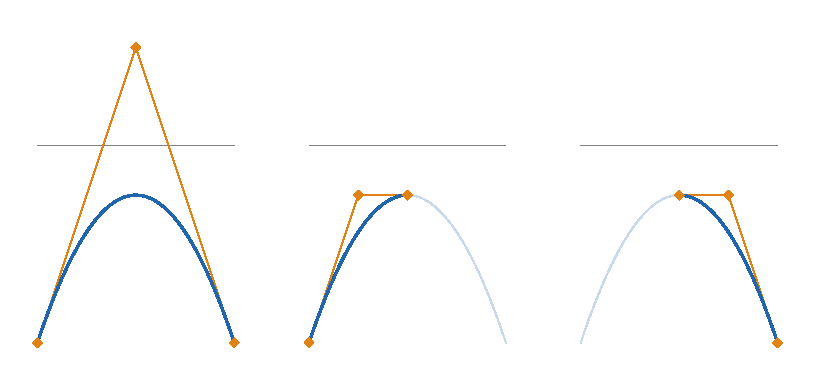
\includegraphics[width=0.85\linewidth]{figures/bernstein}
\caption{\fc{Plug}{The polynomial $p(x)=-1+3x-3x^2$ (blue)}, \fc{Hole}{its Bernstein coefficients (orange diamonds, at $x=l+k(h-l)/2$) and their control polygon}; \fc{Grey}{grey is the axis $p=0$}. Left: on $[0,1]$ the middle coefficient is positive although $p$ is negative throughout, and the sign test refuses. Middle and right: on the two halves, shown with the whole graph for reference, every coefficient is negative and the test succeeds. On each interval the graph lies between the smallest and the largest coefficient.}
\label{fig:bernstein-example}
\end{figure}

\paragraph{Several variables.}
Let $p$ be a polynomial in $x_1,\dots,x_k$ with coefficients in
$\mathbb Q(\sqrt5)$, of degree $n_j$ in $x_j$, and let
$B=\prod_j[l_j,h_j]$ be a closed box with rational endpoints and widths
$w_j=h_j-l_j\ge0$. With $x_j=l_j+w_jy_j$, the products
\[
  B_{\mathbf i}(\mathbf y)=\prod_{j=1}^{k}\binom{n_j}{i_j}
      y_j^{i_j}{(1-y_j)}^{n_j-i_j},
  \qquad 0\le i_j\le n_j,
\]
form a basis of the polynomials of degree at most $n_j$ in each $y_j$.
The unique coefficients $b_{\mathbf i}$ with
\[
  p(l_1+w_1y_1,\dots,l_k+w_ky_k)=\sum_{\mathbf i}b_{\mathbf i}B_{\mathbf i}(\mathbf y)
\]
are the \emph{tensor Bernstein coefficients} of $p$ on $B$; there are
$\prod_j(n_j+1)$ of them.

\begin{lemma}[Bernstein sign test]\label{lem:bernstein-sign-test}
  If every tensor Bernstein coefficient of $p$ on $B$ is strictly
  negative, then $p(\mathbf x)<0$ for every $\mathbf x\in B$.
\end{lemma}
\begin{proof}
  Each $B_{\mathbf i}$ is nonnegative on ${[0,1]}^k$, and their sum is
  $\prod_j{(y_j+(1-y_j))}^{n_j}=1$. A point $\mathbf x\in B$ corresponds to
  $y_j=(x_j-l_j)/w_j$, or to any $y_j\in[0,1]$ when $w_j=0$. So
  $p(\mathbf x)$ is a convex combination of the coefficients and at most
  their maximum, which is negative. This covers every real point of the
  closed box, including its faces and corners and points with irrational
  coordinates.
\end{proof}

The coefficient with every $i_j\in\{0,n_j\}$ is the value of $p$ at the
corresponding corner of $B$. The test therefore refuses a polynomial that
is nonnegative at some corner, and more generally anywhere in $B$. For a
polynomial of degree at most one in each variable, the coefficients are
exactly its corner values, so the test coincides with the endpoint rule of
the Domain component in
\cref{subsec:domain-component-skipping-boxes-outside-the-reduced-domain}.
A refusal never proves anything: it only leaves the box unresolved.

\paragraph{Exact computation.}
The coefficients are computed one variable at a time. Fix $j$, write
$n=n_j$, and expand along $y=y_j$ as
$p=\sum_ka_ky^k$, with coefficients that are polynomials in the other
variables. The identity
\[
  y^k=\sum_{r=k}^{n}\frac{\binom rk}{\binom nk}\binom nr y^r{(1-y)}^{n-r}
\]
converts powers of $y$ into the Bernstein basis, giving
\begin{equation}\label{eq:bernstein-from-power-coefficients}
  b_r=\sum_{k=0}^{r}\frac{\binom rk}{\binom nk}a_k .
\end{equation}
Substitution, expansion and this change of basis use only exact field
operations in $\mathbb Q(\sqrt5)$. In practice we first multiply by a
common denominator, so that every step is an operation on integers of
$\mathbb Z[\sqrt5]$ followed by a known positive scale, and read the sign
of each coefficient with the exact test of
\cref{subsec:exact-representation-of-field-elements-with-integers}.

\paragraph{Convergence under subdivision.}
Refinement helps wherever a polynomial is strictly negative, because the
coefficients approach the values of the polynomial as the box shrinks.

\begin{lemma}[Convergence of Bernstein coefficients]\label{lem:convergence-of-bernstein-coefficients}
  Let $p$ be a polynomial and $K$ a bounded box. There is a constant $C$
  such that for every box $B\subseteq K$ whose widths are all at most
  $w\le1$, every tensor Bernstein coefficient of $p$ on $B$ differs from
  the value of $p$ at the lower corner of $B$ by at most $Cw$. In
  particular, if $p<0$ throughout a closed box $B_*$, every box
  $B\subseteq B_*$ with sufficiently small widths passes the test of
  \cref{lem:bernstein-sign-test}.
\end{lemma}
\begin{proof}
  In one variable, $a_0=p(l)$ and $a_k=p^{(k)}(l)w^k/k!$ by Taylor's
  formula. In \cref{eq:bernstein-from-power-coefficients}, every weight
  lies in $[0,1]$ and the weight of $a_0$ is one, so
  \[
    |b_r-p(l)|\le\sum_{k\ge1}|a_k|
      \le w\sum_{k\ge1}\frac{|p^{(k)}(l)|}{k!}.
  \]
  The derivatives are bounded on $K$. Converting one variable at a time
  applies this bound to polynomials whose coefficients are themselves
  bounded on $K$, and the errors add, giving the constant $C$. For the
  second claim, $p\le-\gamma$ on $B_*$ for some $\gamma>0$ by compactness;
  every coefficient on a subbox of widths at most $w<\gamma/C$ is then at
  most $-\gamma+Cw<0$.
\end{proof}

On a search box, every polynomial we test has degree at most two in each
of the five parameters, so a test inspects at most $3^5=243$ coefficients.
The same test applies after a polynomial change of variables, which is how
the later components use it, through the zoom lemma of
\cref{subsec:the-zoom-lemma}.

% !TEX root = ../main.tex
\pagebreak[0]
\section{\emph{Global} component}\label{sec:global-component}

\begin{figure}[htbp]
\centering
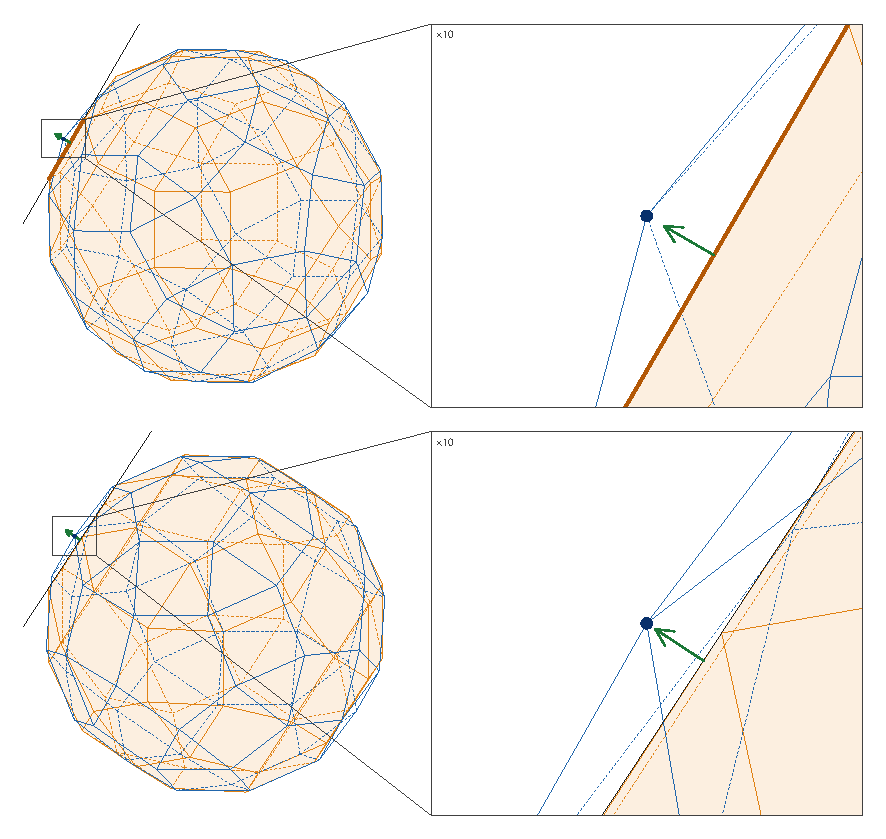
\includegraphics[width=\linewidth]{figures/global}
\caption{Two poke configurations eliminated by the Global component, at the midpoints of two search boxes of the final certificate: $[7/48,7/80,(1/20,-1/20,1/4)]$ and $[3/16,23/80,(-1/40,-13/40,-1/8)]$. Left: the projected edges of \fc{Hole}{the hole (orange)} and of \fc{Plug}{the plug (blue)}, dashed on each body's far side, with \fc{Hole}{the hole's shadow lightly tinted}. Right: the marked windows, enlarged ten times. Black: the supporting line of the hole's shadow for the direction of the hole edge named in the box's record; \fc{Support}{thick brown: the part of the hole's silhouette on that line} (on the right, a single vertex attains it); \fc{Normal}{green: the outward normal}, drawn from the foot of the perpendicular from \fc{Vertex}{the record's plug vertex (dark blue dot)}, which lies strictly beyond the line. The component certifies this separation at every configuration of the box.}
\label{fig:global-examples}
\end{figure}

A projected plug vertex protruding beyond the hole's shadow prevents a fit.
The \emph{Global} component certifies that such protrusion persists
throughout a box. This geometric idea
also underlies the global theorem of
\citet[Section~4, Theorem~17]{SteiningerYurkevichNopertV2}.

\subsection{Eliminating \emph{poke} configurations}\label{subsec:eliminating-poke-configurations}

Fix a poke configuration. At least one projected plug vertex lies outside
the hole's shadow: otherwise convexity would put the entire plug shadow
inside it. We use the orthogonal screen for the separation picture.
There is a direction along which that vertex extends further
than every point of the hole's shadow. To see the comparison, project the
two shadows onto a line parallel to this direction. The selected plug
vertex lies beyond the interval occupied by the hole shadow.

For a nonzero vector $\mathbf n$ in the orthogonal screen plane, the largest
value of $\mathbf n\cdot\mathbf h$ over points $\mathbf h$ of the hole shadow
is its \emph{support value}
in that direction. The line where this value is attained is a
\emph{supporting line}: the whole shadow lies on one side of it.
We call $\mathbf n$ a \emph{support direction}. Since
$\mathbf n\cdot\mathbf u=0$, taking a dot product with $\mathbf n$ gives
the same value before and after projection. Thus a selected plug vertex
$\mathbf v_p\in V$ is separated from the hole shadow if
\begin{equation}\label{eq:point-support-separation}
  \mathbf n\cdot R_P(\mathbf r)\mathbf v_p
     >\max_{\mathbf v\in V}\mathbf n\cdot\mathbf v.
\end{equation}
Due to convexity and the linearity of the dot product, the maximum over
vertices is also the maximum over their convex hull.

\paragraph{Stability of the margin.}
A sufficiently small change of configuration preserves a strict
separation. Before deriving the inequalities used to check a whole box,
we quantify this stability in terms of the margin introduced in
\cref{subsec:the-margin-function-and-fit-poke-touch}.

\begin{lemma}[Lipschitz bound for the margin]\label{lem:lipschitz-bound-for-the-margin}
  For configurations $c,c'\in B_0$,
  \begin{equation}\label{eq:margin-lipschitz-bound}
    |M_{\mathcal R}(c)-M_{\mathcal R}(c')|
       \le16\lVert c-c'\rVert,
  \end{equation}
  where the distance is Euclidean distance between the five parameters,
  as in \cref{subsec:component-hierarchy}.
\end{lemma}
\begin{proof}
  First, $\mathcal R$ contains the ball of radius two about zero and lies
  in the ball of radius five. For the inner bound, average the three cyclic
  permutations of $(1,1,\varphi^3)$, applying the same coordinate sign
  choices to each. This places all eight corners of the cube with half-side
  $(4+\sqrt5)/3>2$ inside $\mathcal R$. For the outer bound, all vertices
  whose coordinates are given in \cref{eq:rhombicosidodecahedron-vertices}
  have distance $\sqrt{11+4\sqrt5}<5$ from the origin. Orthogonal shadows
  therefore give $M_{\mathcal R}(c)\le5/2$ for every configuration.
  The same bound holds in rational screen coordinates: applying the same
  invertible linear map to both shadows preserves scaled containment and
  hence the margin, by \cref{lem:margin-and-containment}.

  \paragraph{Rotation and shadow displacement.}
  We use the Euclidean operator norm for matrices,
  $\lVert A\rVert=\max_{\lVert\mathbf v\rVert=1}\lVert A\mathbf v\rVert$.
  Put $\delta_{s,t}=\lVert(s,t)-(s',t')\rVert$ and
  $\delta_{\mathbf r}=\lVert\mathbf r-\mathbf r'\rVert$. To bound the motion
  of the shadow vertices, we use
  \begin{equation}\label{eq:rotation-and-screen-displacement-bounds}
    \begin{aligned}
      \lVert R_P(\mathbf r)-R_P(\mathbf r')\rVert&\le2\delta_{\mathbf r},\\
      \lVert L_{s,t}-L_{s',t'}\rVert&=\delta_{s,t},\\
      \lVert L_{s,t}\rVert&\le\frac43.
    \end{aligned}
  \end{equation}
  These estimates follow from the rotation and screen formulas
  \cref{eq:relative-rotation,eq:screen-map} and the ranges defining $B_0$.
  For the rotation estimate, write
  ${[\mathbf r]}_\times\mathbf v=\mathbf r\times\mathbf v$. The vector
  triple-product identity gives
  ${[\mathbf r]}_\times^2=\mathbf r\mathbf r^{\mathsf T}-\lVert\mathbf r\rVert^2I$,
  and ${[\mathbf r]}_\times\mathbf r=\mathbf0$. Multiplying by $I-{[\mathbf r]}_\times$
  therefore verifies the inverse formula
  \[
    {(I-{[\mathbf r]}_\times)}^{-1}
      =\frac{I+{[\mathbf r]}_\times+\mathbf r\mathbf r^{\mathsf T}}
             {1+\lVert\mathbf r\rVert^2}.
  \]
  The rotation formula \cref{eq:relative-rotation} can therefore be written as
  \[
    R_P(\mathbf r)=2{(I-{[\mathbf r]}_\times)}^{-1}-I.
  \]
  Also, orthogonality of a cross product to its factors gives
  \[
    \lVert(I-{[\mathbf r]}_\times)\mathbf v\rVert^2
      =\lVert\mathbf v\rVert^2+\lVert {[\mathbf r]}_\times\mathbf v\rVert^2,
  \]
  so this inverse has operator norm at most one. Apply the inverse-difference
  identity $A^{-1}-B^{-1}=A^{-1}(B-A)B^{-1}$ to
  $A=I-{[\mathbf r]}_\times$ and $B=I-{[\mathbf r']}_\times$. Since
  $\lVert\mathbf a\times\mathbf v\rVert\le\lVert\mathbf a\rVert\lVert\mathbf v\rVert$,
  we obtain
  \[
    \lVert R_P(\mathbf r)-R_P(\mathbf r')\rVert
      \le2\lVert {[\mathbf r]}_\times-{[\mathbf r']}_\times\rVert
      \le2\lVert\mathbf r-\mathbf r'\rVert=2\delta_{\mathbf r}.
  \]

  By \cref{eq:screen-map}, the difference $L_{s,t}-L_{s',t'}$ sends
  $\mathbf v$ to $(-(s-s')v_3,-(t-t')v_3)$, so its operator norm is
  $\delta_{s,t}$. Moreover,
  \[
    L_{s,t}L_{s,t}^{\mathsf T}
      =\begin{pmatrix}1+s^2&st\\st&1+t^2\end{pmatrix}
  \]
  has eigenvalues $1$ and $1+s^2+t^2$. The ranges $0\le s\le2/3$ and
  $0\le t\le2/5$ in \cref{eq:search-rectangle} therefore give
  \[
    \lVert L_{s,t}\rVert=\sqrt{1+s^2+t^2}
      \le\sqrt{1+\frac49+\frac4{25}}=\frac{19}{15}<\frac43.
  \]
  Using the vertex bound above, set
  $\delta_H=5\delta_{s,t}$ and
  $\delta_P=5\delta_{s,t}+(40/3)\delta_{\mathbf r}$.
  Corresponding hole vertices satisfy
  \[
    \lVert L_{s,t}\mathbf v-L_{s',t'}\mathbf v\rVert
      \le5\delta_{s,t}=\delta_H.
  \]
  For plug vertices, write the difference as
  \[
    (L_{s,t}-L_{s',t'})R_P(\mathbf r)\mathbf v
      +L_{s',t'}\bigl(R_P(\mathbf r)-R_P(\mathbf r')\bigr)\mathbf v.
  \]
  Rotations preserve length, so the estimates just proved bound its norm by
  \[
    5\delta_{s,t}+\frac43\cdot2\delta_{\mathbf r}\cdot5
      =5\delta_{s,t}+\frac{40}{3}\delta_{\mathbf r}=\delta_P.
  \]
  Taking convex combinations
  of corresponding vertices with the same coefficients gives the same bounds
  for points of the filled shadows, in both directions. Each rational-screen shadow
  contains the radius-two disk, since the spatial body contains the
  radius-two ball and $L_{s,t}(v_1,v_2,0)=(v_1,v_2)$.

  \paragraph{From displacement to margin.}
  Let $m=M_{\mathcal R}(c)$ be the margin at $c$. Each point
  $\mathbf p'\in P_{c'}$ of the plug shadow at $c'$ is within
  $\delta_P$ of some $\mathbf p\in P_c$. Since $P_c\subseteq mH_c$,
  write $\mathbf p=m\mathbf h$ for a point $\mathbf h\in H_c$ of the
  hole shadow at $c$. Choose $\mathbf h'\in H_{c'}$ within
  $\delta_H$ of $\mathbf h$. Then
  \[
    \lVert\mathbf p'-m\mathbf h'\rVert\le m\delta_H+\delta_P.
  \]
  The radius-two disk and convexity of $H_{c'}$ imply
  \[
    P_{c'}\subseteq
    \left(m+\frac{m\delta_H+\delta_P}{2}\right)H_{c'}.
  \]
  Indeed, dividing
  $\mathbf p'=m\mathbf h'+(\mathbf p'-m\mathbf h')$ by the scale factor
  $m+(m\delta_H+\delta_P)/2$ gives a convex combination of
  $\mathbf h'$ and a point in the radius-two disk.
  Apply \cref{lem:margin-and-containment}, use $m\le5/2$, and interchange
  $c,c'$ to obtain
  \begin{equation}\label{eq:margin-from-shadow-displacement}
    |M_{\mathcal R}(c)-M_{\mathcal R}(c')|
      \le\frac{(5/2)\delta_H+\delta_P}{2}
      \le16\lVert c-c'\rVert.
  \end{equation}
  For the exact derivation of the last inequality, substitute the
  displacement bounds above:
  \[
    \frac{(5/2)\delta_H+\delta_P}{2}
      =\frac{35}{4}\delta_{s,t}+\frac{20}{3}\delta_{\mathbf r}.
  \]
  Since the parameter distance is Euclidean,
  $\lVert c-c'\rVert^2=\delta_{s,t}^2+\delta_{\mathbf r}^2$.
  Both $\delta_{s,t}$ and $\delta_{\mathbf r}$ are therefore at most
  $\lVert c-c'\rVert$, and
  \[
    \frac{35}{4}\delta_{s,t}+\frac{20}{3}\delta_{\mathbf r}
      \le\left(\frac{35}{4}+\frac{20}{3}\right)\lVert c-c'\rVert
      =\frac{185}{12}\lVert c-c'\rVert
      \le16\lVert c-c'\rVert.
  \]
\end{proof}

Consequently, if $M_{\mathcal R}(c)=1+\varepsilon$ with $\varepsilon>0$,
then every $c'\in B_0$ with $\lVert c'-c\rVert\le\varepsilon/32$ satisfies
$M_{\mathcal R}(c')\ge1+\varepsilon/2>1$. This gives an explicit neighbourhood consisting entirely of poke
configurations, including when $c$ lies on a boundary of $B_0$.
The constant is a convenient bound derived from the geometry.
The program checks specific support inequalities. We must still prove that those checks
succeed on sufficiently small boxes; we do so in
\cref{subsec:range-and-insufficiency-for-touch-configurations}.

\paragraph{Whole-box support inequalities.}
To choose a support direction that remains perpendicular to the changing
viewing vector, take two distinct hole vertices $\mathbf v_a,\mathbf v_b$
and a sign $\sigma\in\{-1,1\}$, and set
\begin{equation}\label{eq:moving-support-direction}
  \mathbf n(s,t)=\sigma\,\mathbf u\times(\mathbf v_b-\mathbf v_a),
  \qquad \mathbf u=(s,t,1).
\end{equation}
This vector is perpendicular to both the viewing direction and the
segment joining the projected vertices. At a fixed configuration, choosing a pair along a
silhouette edge gives a normal to its supporting line. Throughout a box,
however, the pair need not remain on the silhouette or even be an edge of
the polyhedron: the comparison with every hole vertex is what justifies the result.
If the pair projects to a single point, $\mathbf n=\mathbf0$ and no strict
separation can be certified with it.

Write $\widehat R_P(\mathbf r)=dR_P(\mathbf r)$ for the polynomial
numerator of the rotation, where $d=1+\lVert\mathbf r\rVert^2>0$
is the denominator of the rotation formula.
For each hole vertex $\mathbf v\in V$, define the \emph{gap polynomial}
\begin{equation}\label{eq:support-gap-polynomial}
  p_{\mathbf v}(c)=\mathbf n(s,t)\cdot
    \bigl(\widehat R_P(\mathbf r)\mathbf v_p-d\mathbf v\bigr).
\end{equation}
Its total degree is at most three, and its coefficients lie in
$\mathbb Q(\sqrt5)$. If
\begin{equation}\label{eq:whole-box-support-condition}
  p_{\mathbf v}(c)>0
  \qquad\text{for every }c\in B\text{ and every }\mathbf v\in V,
\end{equation}
then division by $d>0$ proves \cref{eq:point-support-separation}
at every configuration in the box. No hole vertex is singled out: the
comparison with all sixty of them is what justifies the result, so a change
inside the box in which vertices form the silhouette does not by itself
invalidate the test. The certificate record stores the plug vertex and the
ordered hole-vertex pair, whose order fixes the sign; these data determine
all the polynomials to be checked.

\paragraph{Choosing vertices and a support direction.}
Enumerating the vertex pairs from \cref{eq:rhombicosidodecahedron-vertices}
gives exactly 120 pairs at squared distance four. Since the RID has 120
edges, each of length two in the normalisation of
\cref{subsec:the-rhombicosidodecahedron}, this list contains exactly its
edges. Comparing their difference vectors up to sign gives fifteen distinct
unoriented edge vectors. One orientation of each suffices. Reversing the
sign of $\mathbf n$ and replacing the plug vertex $\mathbf v_p$ by its
antipode $-\mathbf v_p$ only permutes the sixty gap polynomials, since
\[
  -\mathbf n\cdot\bigl(\widehat R_P(\mathbf r)\mathbf v_p-d\mathbf v\bigr)
   =\mathbf n\cdot\bigl(\widehat R_P(\mathbf r)(-\mathbf v_p)-d(-\mathbf v)\bigr)
\]
and the vertex set is centrally symmetric. The component therefore
considers $15\times60=900$ candidates: one oriented edge from each class
of parallel edges, with each plug vertex.

Only one candidate is tried on each box. It is chosen in floating point,
as the candidate whose projected plug vertex lies farthest beyond the hole
shadow's extent in the direction $\mathbf n$ at the worst of the box's 32
corners, measured as a distance in the shadow plane. If no candidate lies
beyond at every corner, none is tried. This choice only decides which
exact test to run: a rounding error can make the component try a poorer
candidate and leave the box unresolved, but never eliminate a box. Choosing
at the worst corner rather than at the midpoint matters in practice, as
the midpoint favours candidates that fail near the edges of the box.

\Cref{fig:global-examples} shows two such certified separations, enlarged.

We apply the Bernstein sign test of \cref{subsec:bernstein-coefficients}
to each polynomial $-p_{\mathbf v}$. Testing the differences between plug
and hole values directly preserves cancellations that would be lost by
bounding plug and hole values separately.
Clearing the rotation denominator preserves the inequalities' direction
because $d=1+\lVert\mathbf r\rVert^2\ge1$ for every rotation parameter $\mathbf r$.
Each gap polynomial has degree at most one in $s$ and $t$ and two in each
$r_i$, so each test inspects at most $2\cdot2\cdot3^3=108$ coefficients.

\begin{proposition}[Soundness of the \emph{Global} component]\label{prop:soundness-of-the-global-component}
  Suppose that, for a plug vertex and a signed edge direction, every
  tensor Bernstein coefficient on $B$ of each of the sixty polynomials
  $-p_{\mathbf v}$ in \cref{eq:support-gap-polynomial} is strictly negative.
  Then every configuration in $B$ is a poke configuration, and the box can be eliminated.
\end{proposition}
\begin{proof}
  \Cref{lem:bernstein-sign-test} gives $p_{\mathbf v}>0$ throughout $B$ for
  every hole vertex $\mathbf v$. Dividing by the positive $d$ proves that the
  chosen projected plug vertex lies beyond every projected hole vertex in
  direction $\mathbf n(s,t)$. It therefore lies outside their convex hull, so
  $P_c\nsubseteq H_c$ and $M_{\mathcal R}(c)>1$.
\end{proof}

\subsection{Robustly detecting potential Rupertness}\label{subsec:robustly-detecting-potential-rupertness}

The same support comparisons can identify an unexpected fit during the
search. If $c\in B_0$ and $M_{\mathcal R}(c)=1-\varepsilon$ with
$\varepsilon>0$, then
\cref{lem:lipschitz-bound-for-the-margin} gives
\[
  M_{\mathcal R}(c')\le1-\frac{\varepsilon}{2}<1
  \qquad\text{whenever }c'\in B_0\text{ and }
         \lVert c'-c\rVert\le\frac{\varepsilon}{32}.
\]
This quantifies the openness of the set of fit configurations proved in
\cref{subsec:the-margin-function-and-fit-poke-touch}. Sufficiently deep search boxes
containing $c$ lie entirely in this fitting neighbourhood by
\cref{lem:search-boxes-in-neighbourhoods}, so any point
chosen inside such a box is a fit configuration. We also need an exact
test that recognises it.

\paragraph{Exact detection at a configuration.}
The candidate normals derived from RID edges in \cref{subsec:eliminating-poke-configurations}
supply that test.
Every point outside a convex polygon violates the supporting inequality of
at least one of its edges, because the polygon is the intersection of the
closed half-planes defined by these inequalities.
An edge of the hole shadow is the projection of a supporting face of
$\mathcal R$, obtained by maximizing the corresponding spatial dot product.
Here that face can be a RID edge or one of its polygonal faces.
That face contains a RID edge whose projection is a nonzero segment
parallel to the shadow edge: otherwise all of its edges would project to
points, and so would the face. Hence one of the signed directions in
\cref{eq:moving-support-direction}, using a RID edge, strictly separates
a protruding projected plug vertex.

At a fixed configuration, discard any candidate for which
$\mathbf n=\mathbf0$. A necessary and sufficient condition for fit is
\begin{equation}\label{eq:exact-point-fit-condition}
  \max_{\mathbf v\in V}\mathbf n\cdot\widehat R_P(\mathbf r)\mathbf v
     <d\max_{\mathbf v\in V}\mathbf n\cdot\mathbf v
  \qquad\text{for every remaining candidate }\mathbf n.
\end{equation}
Necessity follows because the compact plug shadow lies in the interior
of the hole shadow, giving a strict support inequality in every nonzero
direction. Conversely, the candidate family includes a normal to every
edge of the hole shadow. Since $d>0$, these strict inequalities put the
entire plug shadow on the inner side of every edge's supporting line,
and hence in the interior of the hole shadow.

Call the left side minus the right side of
\cref{eq:exact-point-fit-condition} the \emph{score} of the candidate; fit
requires every nonzero candidate's score to be negative. At a configuration with rational
parameters, all quantities in \cref{eq:exact-point-fit-condition} lie in
$\mathbb Q(\sqrt5)$. The finite maxima, zero tests and strict comparisons
can therefore be computed exactly using
\cref{subsec:exact-representation-of-field-elements-with-integers}.
The test finishes even when vertices have coincident projections or
several vertices have the same support value; equality between the two
sides of \cref{eq:exact-point-fit-condition} fails the fit condition.
In particular, checking only that no candidate has a
positive score would also accept aligned configurations, whose scores
are all zero.

\paragraph{Detection during subdivision.}
We can add this test to the procedure in
\cref{subsec:boxes-subdivision-and-elimination}: before subdividing an
unresolved box, test its midpoint and stop if it is a fit configuration.
The midpoint is rational because every interval endpoint is rational.
Any other point in the box with rational parameters could be used instead.
The sampled point need not belong to $D$: it still describes a valid
physical configuration, and the containment test applies throughout $B_0$.

\begin{proposition}[Finite detection of fit]\label{prop:finite-detection-of-fit}
  Suppose every elimination component is sound and each component call
  finishes. If the increasing-depth search uses cyclic midpoint subdivision
  and the exact point test above, without a stopping limit, then if a
  fit exists, one is detected after finitely many processed boxes.
\end{proposition}
\begin{proof}
  If a fit exists, \cref{prop:representative-coverage} supplies a fit
  representative $c_*\in D$. No sound component can eliminate a box
  containing $c_*$. Whenever such a box is subdivided, at least one of
  its closed children still contains $c_*$, even if the point lies on
  their shared boundary.

  Write $M_{\mathcal R}(c_*)=1-\varepsilon$, where $\varepsilon>0$.
  By \cref{eq:search-box-diameter-bound}, at a sufficiently large finite
  depth every box containing $c_*$ has diameter less than
  $\varepsilon/32$. Every point in such a box is then a fit configuration
  by the Lipschitz bound above, including its sampled rational point,
  which passes \cref{eq:exact-point-fit-condition}.
  There are finitely many boxes up to that depth, and each component call
  and point test finishes, so increasing-depth processing reaches this
  box and detects a fit unless it has already detected one earlier.
\end{proof}

The sufficient depth depends on the fitting margin, so this argument gives
no uniform practical runtime estimate. On a Nopert input, completion still
requires the elimination components to resolve all boxes.
For bodies without central symmetry, the corresponding search would also
need the translation parameters discussed in
\cref{subsec:projection-containment} and effective exact comparisons for
their vertex coordinates.

The current certificate generator does not run this companion test and
has a finite depth limit; the proposition describes the procedure with
the test added and continued without such a limit.

\subsection{Range and insufficiency for \emph{touch} configurations}\label{subsec:range-and-insufficiency-for-touch-configurations}

For whole-box elimination, finding a separating direction at one
configuration is only the first step: its inequalities must be certified
on the entire box. We describe the range of the component that may try
every one of its 900 candidates. The implementation tries only the
candidate proposed by its floating-point ranking; on boxes drawn uniformly
from the final search, this never lost a box that another candidate
eliminates. The final proof does not rely on either statement: it rests on
the finished certificate, checked as described in
\cref{sec:generating-and-verifying-the-certificate}.

\begin{proposition}[Range of the \emph{Global} component]\label{prop:range-of-the-global-component}
  The range of the Global component is exactly
  \[
    \{c\in B_0:\operatorname{poke}(c)\}.
  \]
\end{proposition}
\begin{proof}
  Fix a poke configuration $c_0$. The edge argument in
  \cref{subsec:robustly-detecting-potential-rupertness} gives a
  plug vertex and signed edge direction for which every gap polynomial
  is strictly positive at $c_0$. By continuity, these sixty polynomials
  remain strictly positive on a closed neighbourhood $U$ of $c_0$ in $B_0$,
  which we may take to be a box. By
  \cref{lem:convergence-of-bernstein-coefficients}, applied to each of them
  on $U$, every box contained in $U$ whose widths are small enough passes
  the test of \cref{prop:soundness-of-the-global-component} with this
  candidate. Shrink $U$ around $c_0$ so that all of its widths are that
  small. Then every search box contained in $U$ is accepted, and $U$
  contains search boxes at arbitrarily large depths by
  \cref{lem:search-boxes-in-neighbourhoods}. This is precisely the range
  condition in \cref{def:range-of-a-component}.

  Conversely, by \cref{prop:soundness-of-the-global-component}, any accepted
  box contains only poke configurations. If $c$ is a fit or touch configuration, no box
  containing it can be accepted. By \cref{lem:search-boxes-in-neighbourhoods},
  every neighbourhood of $c$ contains a search box containing $c$, including
  when $c$ lies on a subdivision boundary. Thus $c$ cannot belong to this
  component's range.
\end{proof}

Together with the compactness reasoning in
\cref{subsec:component-hierarchy}, this shows that sufficiently fine
subdivision handles every compact subset of the set of poke configurations. It does not give
a uniform useful depth as such a subset approaches touch configurations. The Lipschitz
bound quantifies how far the margin remains above one, while the proof above
additionally establishes that the whole-box checks succeed locally.

\paragraph{Limitations at touch configurations.}
At a touch configuration, every projected plug vertex is either inside the
hole shadow or on its silhouette. There is no protrusion, so the component's
strict support inequalities cannot hold throughout a box
containing that configuration. Further subdivision makes these boxes smaller
without removing the touch configuration from every child. Aligned
configurations already provide a whole family of such points.

The next component is designed to eliminate neighbourhoods of aligned
configurations, including the touch configurations themselves, by studying
how the plug's vertices move under sufficiently small relative rotations.

\Cref{fig:global-refinement} shows this on two slices.

\begin{figure}[htbp]
\centering
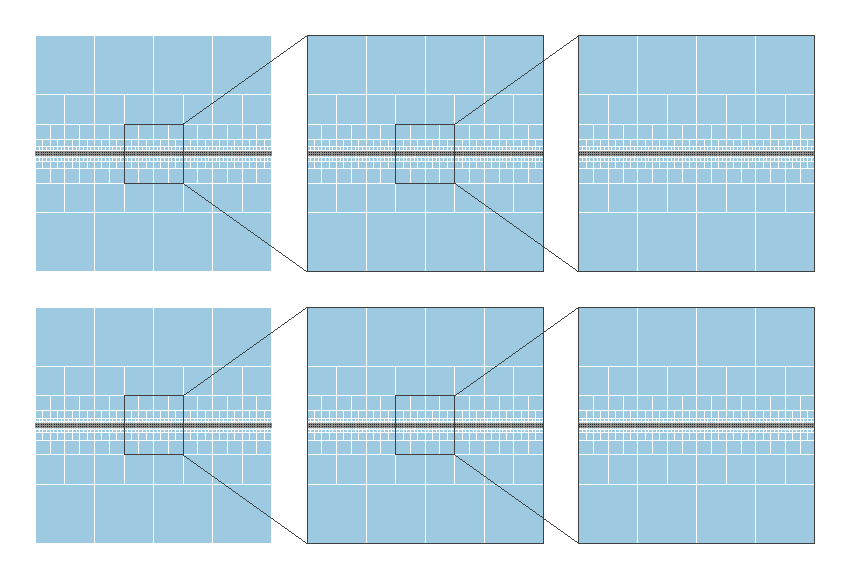
\includegraphics[width=\linewidth]{figures/global-refinement}
\caption{Subdivision with the Domain and Global components alone, near aligned configurations with ordinary viewing directions. Top: the plane $t=1/10$, $r_1=r_2=0$ around $s=1/4$, $r_3=0$ ($s$ horizontally, $r_3$ vertically). Bottom: the plane $s=1/5$, $r_2=r_3=0$ around $t=1/8$, $r_1=0$ ($t$ horizontally, $r_1$ vertically). From left to right, windows of half-width $1/8$, $1/32$ and $1/128$, each halved $14$ times; \fc{Global}{light blue pieces are eliminated by the Global component}, black pieces are unresolved. At every magnification a band of unresolved pieces remains along the aligned configurations: refinement alone never reaches a touch configuration.}
\label{fig:global-refinement}
\end{figure}

% !TEX root = ../main.tex
\section{\emph{Local} component}\label{sec:local-component}

\begin{figure}[htbp]
\centering
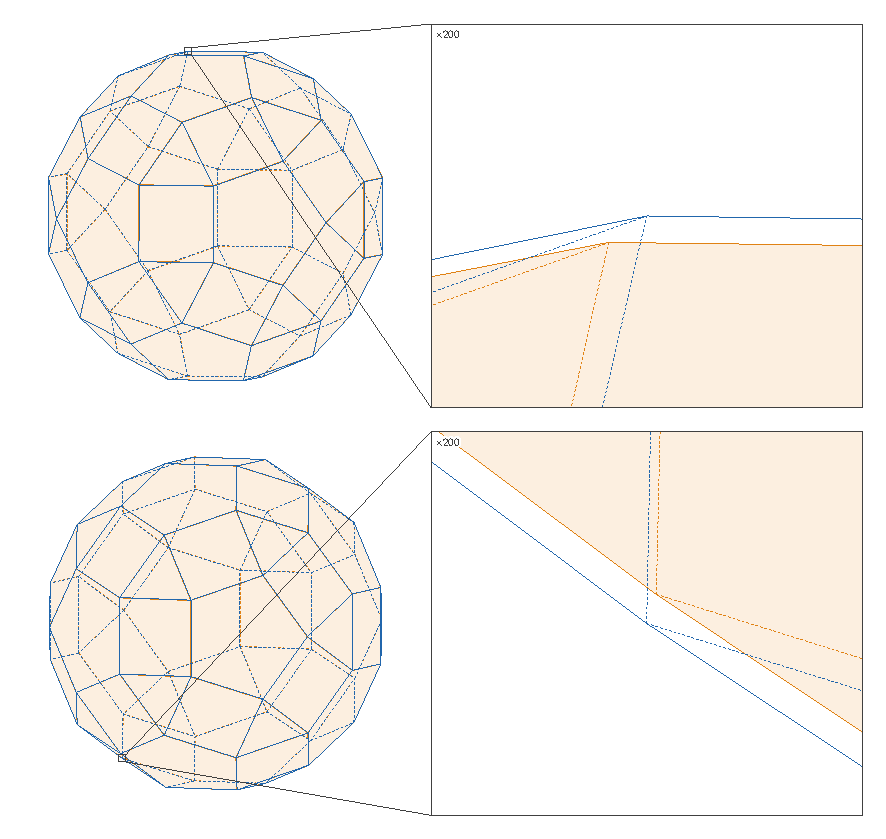
\includegraphics[width=\linewidth]{figures/local}
\caption{Two configurations near aligned ones, in the regions of Local covers: $[1/4,1/20,(1/1000,1/2000,-1/1000)]$ and $[2/5,1/10,(-1/1000,1/1000,1/2000)]$. The \fc{Hole}{hole (orange)} and the \fc{Plug}{plug (blue)} as in \cref{fig:global-examples}. The two shadows almost coincide; the enlargements, $200$ times, show a projected plug vertex protruding beyond the hole's shadow by about $0.004$, the outward motion that the face zooms certify for every small rotation.}
\label{fig:local-examples}
\end{figure}

At an aligned configuration, the plug and hole coincide. A small relative
rotation can nevertheless make a projected plug vertex protrude beyond
the hole's shadow.
The \emph{Local} component uses this outward motion to eliminate whole
neighbourhoods containing aligned configurations, extending the Global component, which
cannot eliminate any box containing an aligned configuration, as established in
\cref{subsec:range-and-insufficiency-for-touch-configurations}.

\subsection{Geometry of \emph{aligned} configurations}\label{subsec:geometry-of-aligned-configurations}

Use the representative $\mathbf r=\mathbf0$ for alignment, so the plug
initially has the hole's orientation. Fix the viewing parameters $(s,t)$
and rotate the plug about a fixed axis through the origin. A vertex
off the axis moves on a circle; its orthogonal projection traces an
ellipse, possibly reduced to a line segment. A vertex on the axis stays
fixed. The rational screen map preserves these descriptions, since it
is an invertible linear change of coordinates on the projection plane.

Choose a vertex whose initial projection lies on a supporting line of
the hole shadow. If its projection moves beyond that line, away from the
hole shadow, the plug cannot fit. We seek a positive interval of rotation
throughout which this protrusion persists, starting immediately after zero rotation.
An outward initial velocity can establish the direction of motion, but
the curvature of the trajectory also matters when determining how far
the plug can rotate before the vertex returns to the supporting line.

For a five-dimensional neighbourhood, this conclusion must hold uniformly
as both $(s,t)$ and the rotation axis vary. Different axes may require
different vertices and supporting lines. We therefore use a finite family
of such choices, each valid throughout a specified region of viewing
parameters and rotation directions. Together they must account for every
direction of rotation and give a common positive bound on its magnitude.
When these bounds hold, they certify that the neighbourhood contains no
fit configurations:
zero-rotation configurations remain touch configurations, while every
nonzero rotation within the bound yields a poke configuration.


\subsection{Eliminating \emph{aligned} configurations}\label{subsec:eliminating-aligned-configurations}

For a nonzero rotation vector $\mathbf r=(r_1,r_2,r_3)$, separate its magnitude
and direction by writing
\begin{equation}\label{eq:normalised-rotation-direction}
  \delta=\lVert\mathbf r\rVert_\infty
         :=\max\{|r_1|,|r_2|,|r_3|\}>0,
  \qquad \widehat{\mathbf r}=\frac{\mathbf r}{\delta},
  \qquad \mathbf r=\delta\widehat{\mathbf r}.
\end{equation}
The normalised vector lies on the boundary of the cube ${[-1,1]}^3$.
We denote its six closed faces by
\[
  F_i^\sigma=\{\widehat{\mathbf r}\in{[-1,1]}^3:
                     \widehat r_i=\sigma\},
  \qquad i\in\{1,2,3\},\quad\sigma\in\{-1,1\}.
\]
On $F_i^\sigma$, coordinate $i$ is fixed at $\sigma$, and the other
two belong to $[-1,1]$.
When several coordinates have maximum absolute value, the vector belongs
to several faces, so the six faces together contain every direction.
The two free face coordinates and $\delta$ describe the three rotational
degrees of freedom.

We use the maximum norm because its unit sphere is made of six squares:
the rotation directions on one face form a box, which is where the
Bernstein sign test works, and a bound on $\delta$ bounds all three
rotation coordinates directly. Here $\widehat{\mathbf r}$ need not have
Euclidean length one, and $\delta$ is not the rotation angle. By
\cref{eq:relative-rotation}, the unit axis and angle are respectively
\[
  \frac{\widehat{\mathbf r}}{\lVert\widehat{\mathbf r}\rVert},
  \qquad
  \theta=2\arctan\bigl(\delta\lVert\widehat{\mathbf r}\rVert\bigr).
\]

\paragraph{Supporting lines throughout a viewing region.}
Fix a closed axis-parallel rectangle $W\subseteq\mathbb R^2$ of viewing
parameters $(s,t)$.
Select a hole vertex $\mathbf v\in V$ and a normal $\mathbf n(s,t)$ perpendicular
to $\mathbf u=(s,t,1)$. For every $(s,t)\in W$,
the projection of $\mathbf v$ must lie on a supporting line of the hole
shadow with outward normal $\mathbf n(s,t)$:
\begin{equation}\label{eq:local-support-conditions}
  \mathbf n(s,t)\cdot(\mathbf w-\mathbf v)\le0
  \qquad\text{for all }\mathbf w\in V.
\end{equation}
As in the Global component, equalities are allowed. Since $\mathbf n\perp\mathbf u$,
the same inequalities compare the orthogonal projections onto the screen.
As the plug rotates, the projection of the vertex starting at $\mathbf v$
protrudes beyond the hole shadow as soon as
$\mathbf n\cdot(R_P(\mathbf r)\mathbf v-\mathbf v)>0$.

The normal must stay perpendicular to $\mathbf u$ as $(s,t)$ varies. We use
either the moving direction \cref{eq:moving-support-direction} of the
Global component, or the direction
\begin{equation}\label{eq:local-fixed-screen-direction}
  \mathbf n(s,t)=(n_1,n_2,-sn_1-tn_2),
  \qquad n_1,n_2\in\mathbb Q(\sqrt5),\quad(n_1,n_2)\ne(0,0),
\end{equation}
which corresponds to the fixed planar support direction $(n_1,n_2)$ in the
screen coordinates $L_{s,t}$ of \cref{eq:screen-map}. For either form, each
of the sixty inequalities in \cref{eq:local-support-conditions} is affine
in $(s,t)$, so checking them at the four corners of $W$ establishes
support throughout $W$.

\paragraph{Displacement under rotation.}
To determine how long this protrusion persists,
we need both its initial direction of motion and the bending of its
circular trajectory. For a vertex off the rotation axis,
$\widehat{\mathbf r}\times\mathbf v$ points along the initial tangent,
while $\widehat{\mathbf r}\times(\widehat{\mathbf r}\times\mathbf v)$
points towards the axis. Taking their components along the outward
normal gives the two displacement polynomials
\begin{equation}\label{eq:local-displacement-polynomials}
  p_1=\mathbf n\cdot(\widehat{\mathbf r}\times\mathbf v),
  \qquad
  p_2=\mathbf n\cdot
       \bigl(\widehat{\mathbf r}\times
                    (\widehat{\mathbf r}\times\mathbf v)\bigr).
\end{equation}
Their variables are $s,t$ and the two free coordinates of
$\widehat{\mathbf r}$ on $F_i^\sigma$. A positive $p_1$ indicates
initial outward motion, whereas a negative $p_2$ opposes it as the
rotation grows. Subtracting $\mathbf v$ from
\cref{eq:relative-rotation}, substituting
$\mathbf r=\delta\widehat{\mathbf r}$, and using
\[
  \widehat{\mathbf r}\times
    (\widehat{\mathbf r}\times\mathbf v)
  =\widehat{\mathbf r}(\widehat{\mathbf r}\cdot\mathbf v)
     -\lVert\widehat{\mathbf r}\rVert^2\mathbf v
\]
gives the exact identity
\begin{equation}\label{eq:local-radial-displacement}
  \mathbf n\cdot
    \bigl(R_P(\delta\widehat{\mathbf r})\mathbf v-\mathbf v\bigr)
   =\frac{2\delta}
          {1+\delta^2\lVert\widehat{\mathbf r}\rVert^2}
       (p_1+\delta p_2).
\end{equation}

\paragraph{Dividing out the size of the rotation.}
Both sides of \cref{eq:local-radial-displacement} vanish at $\delta=0$,
where the configuration is aligned. This is why no box containing an
aligned configuration can be eliminated by testing the displacement
directly: its sign is zero there, and the Bernstein sign test must refuse
it. The factor $\delta$, however, is explicit. In terms of the gap
polynomial \cref{eq:support-gap-polynomial} of the Global component,
with the plug vertex $\mathbf v_p=\mathbf v$ and the rotation denominator
$d=1+\delta^2\lVert\widehat{\mathbf r}\rVert^2$, the identity reads
\begin{equation}\label{eq:local-gap-factorisation}
  p_{\mathbf v}
   =\mathbf n\cdot\bigl(\widehat R_P(\delta\widehat{\mathbf r})\mathbf v-d\mathbf v\bigr)
   =2\delta\,(p_1+\delta p_2),
\end{equation}
an identity of polynomials in $s$, $t$, $\delta$ and the two free
coordinates of $\widehat{\mathbf r}$. If the quotient $2(p_1+\delta p_2)$
is positive throughout a closed region of these five variables with
$0\le\delta\le\delta_{\max}$, then the vertex protrudes at every
positive $\delta$ in the region, and the configurations with $\delta=0$ are
aligned touch configurations, which are not fits. The Bernstein sign test
can certify the quotient directly, and it can succeed even at $\delta=0$,
where the quotient is $2p_1$: it only needs outward initial motion.

This observation is the idea behind every remaining component of the
proof. Near a set of configurations that are already known not to be fits,
we change coordinates so that some coordinates measure the distance from
that set, divide a necessary inequality exactly by a power of those
distances, and certify the quotient with Bernstein coefficients.

\subsection{The zoom lemma}\label{subsec:the-zoom-lemma}

The rest of the proof uses the same step with other sets in place of the
aligned configurations and other distances in place of $\delta$. We
therefore state it once, in a form that covers every use.

Several of the coordinate changes below scale the viewing direction, so we
allow the viewing vector to be any positive multiple of $(s,t,1)$: a vector
$\mathbf u$ with $u_3>0$ and a rotation vector $\mathbf r$ describe the
configuration $[u_1/u_3,u_2/u_3,\mathbf r]$.

\begin{definition}[No-fit sets and witnesses]\label{def:witness}
  A \emph{no-fit set} is a set of configurations containing no fit.
  A \emph{witness} is a polynomial $p$ in $\mathbf u$ and $\mathbf r$,
  homogeneous in $\mathbf u$, together with finitely many linear forms
  $\lambda_1,\dots,\lambda_m$ in $\mathbf u$, possibly none, its
  \emph{validity conditions}, such that $p\le0$ at every fit in $D$
  whose viewing vector satisfies $\lambda_j(\mathbf u)\ge0$ for all $j$.
\end{definition}

By homogeneity, the signs of $p$ and of each $\lambda_j$ do not depend on
the positive multiple chosen for $\mathbf u$. The aligned configurations form
a no-fit set: by \cref{eq:relative-rotation}, $\mathbf r=\mathbf0$ gives
$P_c=H_c$, and a compact shadow never lies in its own interior. Two kinds
of witnesses suffice for the whole proof.
\begin{itemize}
  \item A gap polynomial \cref{eq:support-gap-polynomial}, with
    $\mathbf n$ written as a linear function of $\mathbf u$ (for
    \cref{eq:local-fixed-screen-direction}, as
    $(u_3n_1,u_3n_2,-u_1n_1-u_2n_2)$), whose validity conditions are the
    support inequalities \cref{eq:local-support-conditions} of its hole
    vertex $\mathbf v$. Where they hold, the projection of $\mathbf v$ lies on
    a supporting line of the hole shadow with outward normal $\mathbf n$; a fit
    puts the projected plug vertex in the interior of the hole shadow, strictly
    on the inner side of that line, so the gap polynomial is negative there.
  \item A \emph{domain polynomial}: the polynomial $q$ of an inequality
    $q\le0$ defining $D$, written homogeneously in $\mathbf u$ (the fold
    inequality, for example, as ${\ell_g}^2-\lVert\mathbf u\rVert^2$), without
    validity conditions. It is nonpositive on all of $D$.
\end{itemize}

\begin{definition}[Zooms]\label{def:zoom}
  A \emph{zoom} is a polynomial map $\mathcal Z$ from a box $Y$ of
  \emph{zoom coordinates} $\mathbf y=(y_1,\dots,y_5)$ to viewing and
  rotation vectors, $\mathcal Z(\mathbf y)=(\mathbf u(\mathbf y),\mathbf r(\mathbf y))$,
  together with a set of designated \emph{distance coordinates}, such that
  \begin{enumerate}
    \item $u_3(\mathbf y)>0$ on $Y$, and each component of
      $\mathbf u(\mathbf y)$ has degree at most one in each zoom coordinate;
    \item each distance coordinate is nonnegative on $Y$, and wherever one
      of them vanishes, $\mathcal Z(\mathbf y)$ lies in a fixed no-fit set,
      the zoom's no-fit set.
  \end{enumerate}
  A monomial $\mathbf y^{\mathbf a}=\prod_jy_j^{a_j}$ in the distance
  coordinates is a \emph{zoom factor}, and a closed box $C\subseteq Y$ is a
  \emph{zoom cell}.
\end{definition}

The name describes what a zoom does near its no-fit set. A distance
coordinate measures how far a configuration is from that set, and the
other coordinates describe the direction of departure in units of that
distance. A thin neighbourhood of the no-fit set is thereby spread out
over a whole box, much as a camera zooms in on a detail, and once the zoom
factor is divided out, the behaviour of a witness arbitrarily close to the
no-fit set becomes the behaviour of a polynomial on a box, where Bernstein
coefficients can see it. The degree condition in the first requirement is
what allows validity conditions to be checked at the corners of a cell.

\begin{lemma}[Zoom lemma]\label{lem:zoom-lemma}
  Let $\mathcal Z$ be a zoom, $C$ a zoom cell and $p$ a witness. Suppose that
  \begin{enumerate}
    \item $p(\mathcal Z(\mathbf y))=\mathbf y^{\mathbf a}N(\mathbf y)$ exactly,
      as polynomials, for a zoom factor $\mathbf y^{\mathbf a}$;
    \item every validity condition of $p$ holds at the viewing vectors
      $\mathbf u(\mathbf y)$ of the corners $\mathbf y$ of $C$;
    \item every tensor Bernstein coefficient of $N$ on $C$ is strictly
      positive.
  \end{enumerate}
  Then no configuration $\mathcal Z(\mathbf y)$ with $\mathbf y\in C$ is a
  fit lying in $D$. More precisely, each such configuration lies in the
  zoom's no-fit set or satisfies $p>0$ and the validity conditions of $p$;
  for a gap polynomial, the latter makes it a poke configuration.
\end{lemma}
\begin{proof}
  By \cref{lem:bernstein-sign-test} applied to $-N$, we have $N>0$
  throughout $C$. Let $\mathbf y\in C$. If a distance coordinate with
  $a_j>0$ vanishes at $\mathbf y$, then $\mathcal Z(\mathbf y)$ lies in the
  no-fit set. Otherwise $\mathbf y^{\mathbf a}>0$, so
  $p(\mathcal Z(\mathbf y))>0$, and by homogeneity $p>0$ at the
  configuration itself. Each validity condition $\lambda_j(\mathbf u(\mathbf y))$
  is linear in $\mathbf u$, and $\mathbf u(\mathbf y)$ has degree at most one
  in each zoom coordinate, so the condition is affine in each coordinate
  separately; varying one coordinate at a time, its minimum over $C$ is
  attained at a corner. The validity conditions therefore hold throughout
  $C$, and since $p$ is a witness, $p>0$ excludes a fit in $D$. For a gap
  polynomial, $p>0$ places the projected plug vertex strictly beyond a
  supporting line of the hole shadow.
\end{proof}

The lemma separates what is proved by hand from what is checked by the
computer. By hand: that a set is a no-fit set, that a polynomial is a
witness, and that the zooms reach every configuration of the region
concerned. By exact computation, cell by cell: the division, the validity
conditions at the corners and the signs of the Bernstein coefficients.
The division must be exact; a single term that is not a multiple of the
zoom factor means the cell is refused.

The tests of the preceding components are the simplest case, with nothing
divided out. With the identity map on a search box as the zoom, no distance
coordinates and the zoom factor one, the lemma for a domain polynomial is
exactly the test of the Domain component. The test of the Global component
is the same idea for gap polynomials, except that instead of checking the
validity conditions of one hole vertex at the corners, it requires the gap
polynomials of all sixty hole vertices to be positive, so that whichever
hole vertex supports the shadow, its gap polynomial is positive.

\paragraph{Tube zooms.}
The zooms of this paper are of two kinds. Both use coordinates adapted to a
no-fit set: after an invertible affine change of variables, the
\emph{base} coordinates $\mathbf z_b$ run along the no-fit set and the
\emph{offset} coordinates $\mathbf z_o$ measure the displacement away from
it, so that the configurations with $\mathbf z_o=\mathbf0$ lie in the no-fit
set. As for the rotation vector above, the offsets are normalised on the
faces of a box. Let $\Phi\subseteq{[-1,1]}^m$ be a box whose every side is
$[-1,0]$, $[0,1]$ or $[-1,1]$; a side $[0,1]$ or $[-1,0]$ records that an
offset coordinate has a fixed sign. The \emph{cone} of $\Phi$ is the set of
vectors whose coordinates have the signs that $\Phi$ allows: nonnegative
where its side is $[0,1]$, nonpositive where it is $[-1,0]$. For
$\mathbf z\ne\mathbf0$ in the cone, $\mathbf z/\lVert\mathbf z\rVert_\infty$
lies on a \emph{face} of $\Phi$, a side where one coordinate equals $\pm1$.

Let the base coordinates range over a box $\Sigma_b$, and let
$\delta_{\max}>0$. For each face $F$ of $\Phi$, the \emph{tube zoom}
$\mathcal T_F$ has as zoom coordinates the base coordinates
$\mathbf z_b\in\Sigma_b$, the distance coordinate $\delta\in[0,\delta_{\max}]$
and the free coordinates of $\widehat{\mathbf f}\in F$, and it sets
$\mathbf z_o=\delta\widehat{\mathbf f}$. The \emph{covered set} of the
family is
\begin{equation}\label{eq:tube-covered-set}
  \{(\mathbf z_b,\mathbf z_o):\ \mathbf z_b\in\Sigma_b,\ \mathbf z_o\in\delta_{\max}\Phi\}.
\end{equation}

\begin{lemma}[Tube coverage]\label{lem:tube-coverage}
  Every configuration in the covered set of a family of tube zooms lies in
  the no-fit set or is the image of a point in the domain of one of them.
\end{lemma}
\begin{proof}
  Let $\delta=\lVert\mathbf z_o\rVert_\infty\le\delta_{\max}$. If $\delta=0$, the
  configuration lies in the no-fit set. Otherwise
  $\widehat{\mathbf f}=\mathbf z_o/\delta$ lies on a face $F$ of $\Phi$, and
  $(\mathbf z_b,\delta,\widehat{\mathbf f})$ is a point of the domain of
  $\mathcal T_F$.
\end{proof}

Tube zooms divide out one distance, the size of the offset. They are used
around the aligned configurations below and along two families of
non-aligned touch configurations in \cref{sec:arc-configurations}. At a few
special points, one distance is not enough, and
\cref{sec:square-and-pentagon-configurations} introduces \emph{point zooms},
which divide out two: the distance along the no-fit set from the special
point, and the offset measured relative to it. Where two families of touch
configurations cross, \cref{sec:endpoint-and-crossing-configurations} adds
a \emph{hand-over} from zooms around one family to zooms around the other.

\paragraph{Zoom covers.}
The cells of a family of zooms are found by subdivision. The domain of
each zoom is bisected in one coordinate at a time, keeping both children,
until every terminal cell carries a witness and a zoom factor satisfying
the hypotheses of \cref{lem:zoom-lemma}. The union of the children is their
parent, so by induction the terminal cells cover the domain. A family of
zooms with such subdivisions and witnesses is a \emph{zoom cover}; its
covered set is the covered set of its family. The cells and witnesses are
found by the program's generator (\texttt{rid generate}), but every cell is checked exactly before use,
so how they were found does not matter.

\subsection{Face zooms and the \emph{Local} component}\label{subsec:face-zooms-and-the-local-component}

The \emph{face zooms} are the tube zooms around the aligned
configurations. Their base coordinates are the viewing parameters
$(s,t)\in W$, their offset is the rotation vector $\mathbf r$ with
$\Phi={[-1,1]}^3$, whose six faces are the $F_i^\sigma$, and
\[
  \mathbf u=(s,t,1),\qquad \mathbf r=\delta\widehat{\mathbf r},
  \qquad \widehat{\mathbf r}\in F_i^\sigma,\quad 0\le\delta\le\delta_{\max}.
\]
Where the distance coordinate $\delta$ vanishes, $\mathbf r=\mathbf0$ and the
configuration is aligned. By \cref{eq:local-gap-factorisation}, a gap
polynomial whose plug vertex is its hole vertex is divisible by the zoom
factor $\delta$. The same holds for any plug vertex $\mathbf v_p$ whose
unrotated projection lies on the same supporting line throughout the cell,
for example the other end of a hole edge along it, since the gap then
vanishes at $\delta=0$; the exact division checks this. The covered set of
the six face zooms is the region
\begin{equation}\label{eq:local-region}
  W\times{[-\delta_{\max},\delta_{\max}]}^3 .
\end{equation}

\begin{proposition}[Soundness of the \emph{Local} component]\label{prop:soundness-of-the-local-component}
  Suppose a zoom cover of face zooms with covered set \cref{eq:local-region}
  has been checked, with a gap polynomial and a zoom factor $\delta$ or $1$ in
  every cell. Then every configuration in that region is a touch
  configuration when $\mathbf r=\mathbf0$ and a poke configuration
  otherwise. Any search box contained in the region can therefore be
  eliminated.
\end{proposition}
\begin{proof}
  By \cref{lem:tube-coverage}, a configuration of the region with
  $\mathbf r\ne\mathbf0$ is the image of a point of some face zoom's domain,
  and a terminal cell contains this point. By \cref{lem:zoom-lemma}, the
  cell's witness is positive there, so a projected plug vertex lies strictly
  beyond a supporting line of the hole shadow and the configuration is a
  poke configuration. Zero rotation yields an aligned and therefore touch
  configuration.
\end{proof}

\paragraph{Checking a search box.}
The Local component has a finite list of viewing rectangles $W$ with
checked zoom covers and bounds $\delta_{\max}$. It accepts a search box that
lies in one of the regions \cref{eq:local-region}: the product of its two
viewing intervals must lie in $W$, and each of its three rotation intervals
in $[-\delta_{\max},\delta_{\max}]$. Its certificate record names the
region, so that these endpoint comparisons can be repeated. The covers are
checked once, before the search; the test for a box is only this
inclusion. \Cref{fig:local-refinement} shows the effect of adding the Local
component.

\begin{figure}[htbp]
\centering
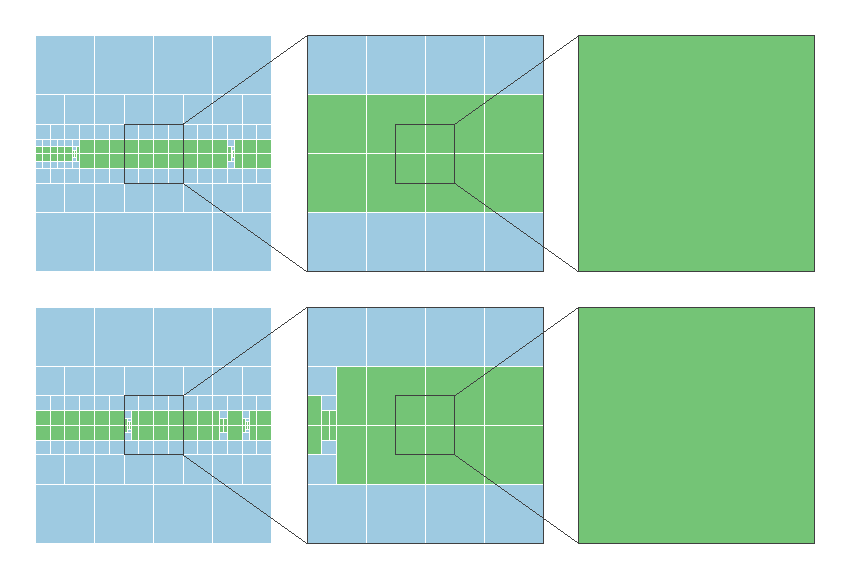
\includegraphics[width=\linewidth]{figures/local-refinement}
\caption{The slices of \cref{fig:global-refinement} with the \fc{Local}{Local component added (green)}. The unresolved band is gone: near the aligned configurations every piece lies in the region of a Local cover, and in the smallest window the whole window does at once.}
\label{fig:local-refinement}
\end{figure}

\subsection{Range and exotic viewing directions}\label{subsec:range-and-exotic-viewing-directions}

The Local component has 30 zoom covers of this kind, with bounds
$\delta_{\max}$ between $1/200$ and $1/20$ and 833 terminal cells in all.
Their viewing rectangles come from 30 rectangles with disjoint interiors,
each enlarged by $1/1024$ on every side (and cut to the viewing rectangle
$[0,2/3]\times[0,2/5]$ of $B_0$), so that neighbouring rectangles overlap and
a small search box on the boundary between two of them lies inside one.
For example, one of the regions is
\[
  \left[\frac16-\frac1{1024},\frac13+\frac1{1024}\right]\times
  \left[0,\frac1{10}+\frac1{1024}\right]\times
  {\left[-\frac1{50},\frac1{50}\right]}^3.
\]
Since $\lVert\mathbf r\rVert_\infty\le\lVert\mathbf r\rVert=\tan(\theta/2)$,
such a region contains the rotations about every axis through angles
$0\le\theta\le2\arctan\delta_{\max}$.

The relative interior in $B_0$ of each region lies in the Local component's
range (\cref{def:range-of-a-component}): every configuration there has a
neighbourhood inside the region, and every search box within that
neighbourhood passes the inclusion test. In
\cref{subsec:ranges-and-remaining-touch-configurations} we show that these
regions, together with the covers of the next section, contain a
neighbourhood of every aligned configuration of $D$.

\paragraph{Exotic viewing directions.}
The rectangles leave out two viewing directions, and no face zoom cover can
reach them. At each of them, for every vertex and every supporting line
valid throughout a neighbourhood of that viewing direction, the quotient
$2p_1$ in \cref{eq:local-gap-factorisation} vanishes at $\delta=0$ for some
rotation directions, so no face zoom cell
containing them can pass the test, however small. Both are directions from
which faces of the RID are seen edge-on: the direction $(s,t)=(0,0)$, along
which the four square faces with normals $\pm\mathbf e_1$ and $\pm\mathbf e_2$
are seen edge-on, and a direction on the boundary of the viewing triangle
from which a pentagonal face is seen edge-on. Near such a direction, a
small change of the viewing direction changes which vertices of the
edge-on faces belong to the silhouette, and supports that work on one side
fail on the other. We located the two directions by subdivision: with the
Global and Local components alone, the unresolved boxes concentrate around
them (\cref{fig:exotic-directions}).
\Cref{sec:square-and-pentagon-configurations} divides out a second distance
there.

\begin{figure}[htbp]
\centering
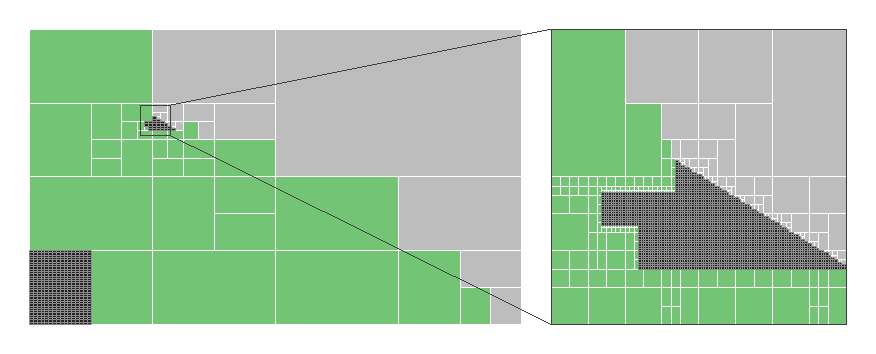
\includegraphics[width=\linewidth]{figures/exotic-directions}
\caption{The plane $\mathbf r=\mathbf 0$ of aligned configurations, with $s\in[0,2/3]$ horizontally and $t\in[0,2/5]$ vertically, halved $14$ times with the \fc{Domain}{Domain (grey)}, Global and \fc{Local}{Local (green)} components; right, the window of half-width $1/48$ around the point where the edge-on line $s=(\varphi-1)t$ meets the long side of the viewing triangle. Every configuration of this plane is a touch configuration, so the Global component eliminates none of it: beyond the viewing triangle the Domain component removes it, and inside only the Local covers eliminate pieces. They reach every viewing direction of the triangle except those near the corner $(0,0)$ and near that point, where the pieces stay unresolved (black) at any depth.}
\label{fig:exotic-directions}
\end{figure}

% !TEX root = ../main.tex
\pagebreak[0]
\section{\emph{Square} and \emph{pentagon} configurations}\label{sec:square-and-pentagon-configurations}

\begin{figure}[htbp]
\centering
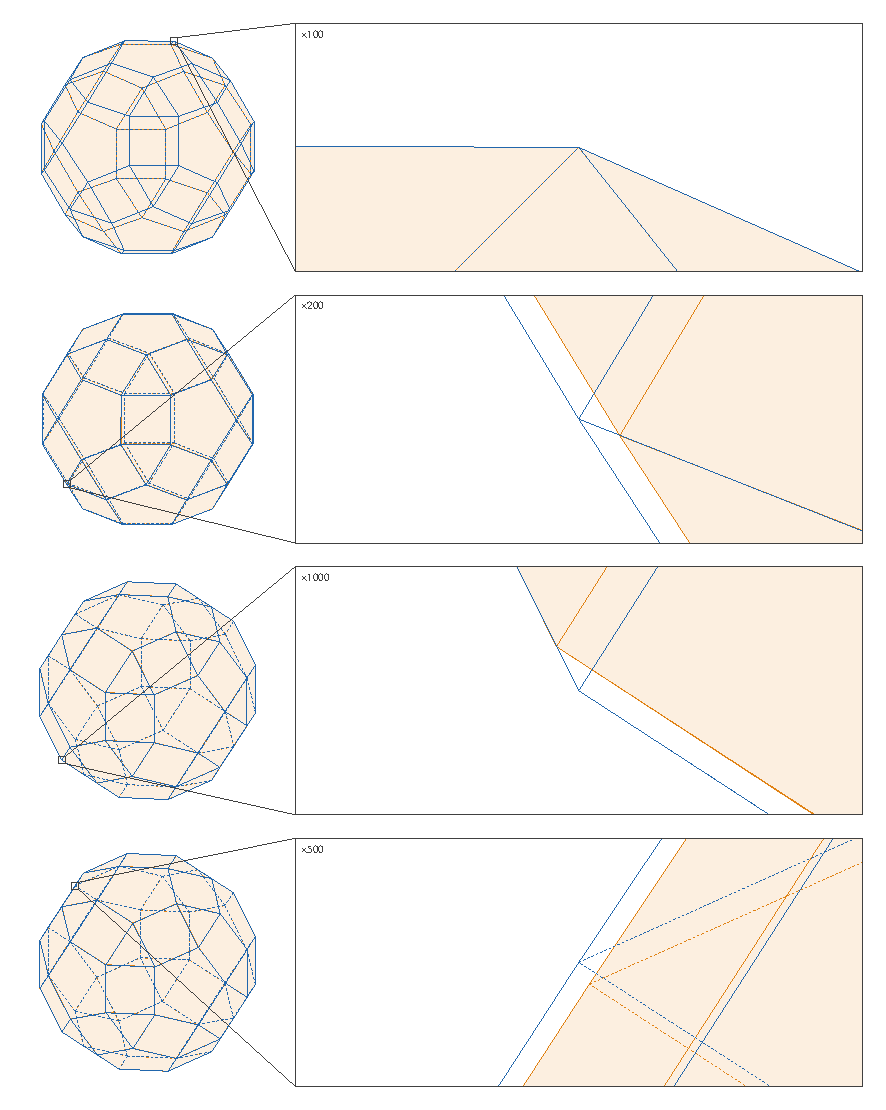
\includegraphics[width=\linewidth]{figures/square-pentagon}
\caption{Near the square configuration (top two rows) and the pentagon configuration (bottom two); the \fc{Hole}{hole (orange)} and the \fc{Plug}{plug (blue)} as in \cref{fig:global-examples}. First: the configuration $[1/16,1/16,(-1/16,1/16,0)]$ of the half-turn family, whose plug shadow and projected edges coincide with the hole's, so that a single wireframe is visible, enlarged $100$ times at a vertex of the outline; it lies outside $D$. Second: the poke configuration $[1/64,1/128,(1/1000,-1/1000,-1/1000)]$, with a plug vertex protruding by about $0.005$ (enlarged $200$ times). Third and fourth: the viewing parameters $(\eta,\xi)=(1/200,-1/400)$ and $(-1/200,-1/400)$ of \cref{subsec:eliminating-the-pentagon-configuration}, on the two sides of the line along which a pentagonal face is seen edge-on, with the rotation $\mathbf r=(1/1000,0,0)$; a different plug vertex protrudes on each side (enlarged $1000$ and $500$ times).}
\label{fig:square-pentagon-examples}
\end{figure}

The two viewing directions left out by the Local component belong to two
aligned configurations. We call the aligned configuration with
$(s,t)=(0,0)$ the \emph{square} configuration: its viewing line passes
through opposite square faces. The second, the \emph{pentagon}
configuration, has
\begin{equation}\label{eq:pentagon-viewing-parameters}
  (s,t)=\left(\frac{-5+3\sqrt5}{10},\frac{5-\sqrt5}{10}\right),
\end{equation}
where the boundary $\varphi s+\varphi^2t=1$ of the viewing triangle meets
the line $s=(-1+\varphi)t$, along which a pentagonal face with normal
$(1,1-\varphi,0)$ is seen edge-on.

Three things make these configurations harder than the other aligned
ones, and the rest of the section deals with them in turn.
\begin{enumerate}
  \item At both, for every vertex and supporting line valid near the special
    viewing direction, the initial outward motion vanishes for some
    directions of rotation, and dividing out the size of
    the rotation is not enough. \emph{Point zooms}, below, divide out a
    second distance: the distance of the viewing parameters from those of
    the special configuration.
  \item At the square configuration, a family of touch configurations with
    nonzero rotation reaches the aligned configuration. The fold
    inequalities of \cref{eq:reduced-domain} remove it
    (\cref{subsec:eliminating-the-square-configuration}).
  \item At the pentagon configuration, the vertices of the edge-on face that
    form the silhouette differ on the two sides of the edge-on line, and so
    do the useful supports (\cref{subsec:eliminating-the-pentagon-configuration}).
\end{enumerate}
Both configurations are handled by one further component, the
\emph{Exotic} component. Like the Local component, it eliminates a
search box by checking that the box lies in the covered set of a zoom
cover that was checked once, before the search. It has two covers here,
one around each configuration, and six more in
\cref{sec:arc-configurations,sec:endpoint-and-crossing-configurations}.

\paragraph{Why one distance is not enough.}
A model shows the difficulty. Let $x\ge0$ measure how far the viewing
parameters are from those of the special configuration, and let $y\ge0$
be the size of the rotation. Suppose a witness behaves like
\[
  p=y(x+y).
\]
A face zoom divides by $y$ and leaves $x+y$, which is positive except at
$x=y=0$, where it vanishes. No zoom cell containing the special
configuration can then pass the test of \cref{lem:zoom-lemma}, however
small. The Local component meets exactly this behaviour at the square and
pentagon configurations: in the directions of rotation described in
\cref{subsec:range-and-exotic-viewing-directions}, the initial
outward motion of every projected vertex, measured against any support
valid near the special configuration, is proportional to $x$.

\paragraph{Point zooms.}
The remedy is to measure the rotation relative to $x$, using two families
of zooms around the special configuration (\cref{fig:toy-zoom}).
\begin{itemize}
  \item In \emph{family A}, the rotation is at most $\rho_0$ times the
    distance of the viewing parameters: that distance is $\mu$, and the
    rotation has size $\rho\mu$ with $0\le\rho\le\rho_0$. Both $\mu$ and
    $\rho$ are distance coordinates. In the model, $p=\mu^2\rho(1+\rho)$.
  \item In \emph{family B}, the rotation is larger: its size is $\delta$ and
    the distance of the viewing parameters is $b\delta$ with
    $0\le b\le1/\rho_0$. The distance coordinate is $\delta$. In the model,
    $p=\delta^2(b+1)$.
\end{itemize}
After division by the zoom factors $\mu^2\rho$ and $\delta^2$, both
quotients are at least one throughout their zoom boxes, including the
special configuration itself, which has become the whole face $\mu=0$ or
$\delta=0$. The ratio $\rho_0>0$ is a parameter; any positive value works in
the model.

\begin{figure}[htbp]
\centering
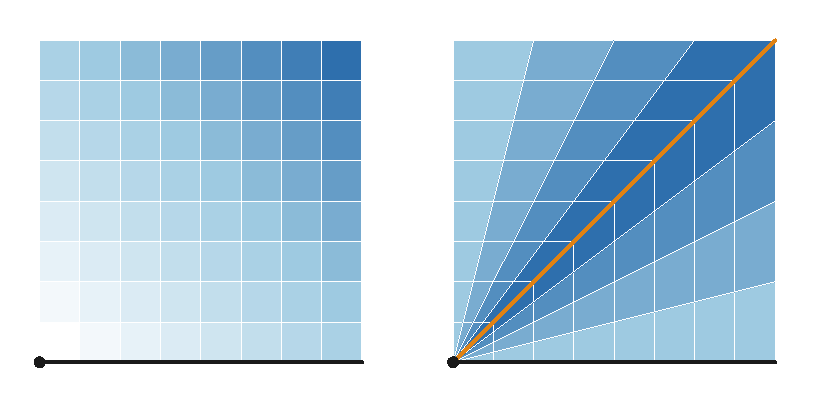
\includegraphics[width=0.9\linewidth]{figures/toy-zoom}
\caption{The model $p=y(x+y)$: the distance $x\ge0$ of the viewing parameters horizontally and the size $y\ge0$ of the rotation vertically, both in $[0,1]$; the no-fit set $y=0$ is the black line and the special configuration the black dot. Each cell is shaded by the smallest value of its quotient, from white for $0$ to \fc{Quotient}{dark blue for $2$}. Left: the cells of a face zoom, which divides by $y$; the quotient $x+y$ fades to $0$ at the special configuration, so the cell there fails however small it is. Right: the point zooms with $\rho_0=1$. Below \fc{Hole}{the diagonal (orange)}, family A, with the segments of constant distance $\mu$ and the rays of constant ratio $\rho$; above it, family B, with the segments of constant rotation size $\delta$ and the rays of constant ratio $b$. The quotients $1+\rho$ and $1+b$ are at least $1$ on every cell, including the cells at the special configuration.}
\label{fig:toy-zoom}
\end{figure}

In general, we use base and offset coordinates as for the tube zooms of
\cref{subsec:the-zoom-lemma}, now around a point: the special configuration
is $\mathbf z_b=\mathbf z_o=\mathbf0$, and the configurations with
$\mathbf z_o=\mathbf0$ lie in the no-fit set. Both parts are normalised on
the faces of boxes: the offsets on the faces of a box
$\Phi\subseteq{[-1,1]}^m$, and the base directions on the faces of a box
$\Sigma\subseteq{[-1,1]}^{5-m}$, each with sides $[-1,0]$, $[0,1]$ or
$[-1,1]$.

Given a base radius $\mu_{\max}$, an offset radius $\delta_{\max}$ and the
ratio $\rho_0$, the \emph{point zooms} are
\begin{itemize}
  \item $\mathcal A_{G,F}$, for each face $G$ of $\Sigma$ and $F$ of $\Phi$:
    $\mathbf z_b=\mu\widehat{\mathbf b}$ and
    $\mathbf z_o=\rho\mu\widehat{\mathbf f}$, with $\widehat{\mathbf b}\in G$,
    $\widehat{\mathbf f}\in F$, $0\le\mu\le\mu_{\max}$ and $0\le\rho\le\rho_0$;
  \item $\mathcal B_F$, for each face $F$ of $\Phi$: $\mathbf z_b=\delta\mathbf b$
    and $\mathbf z_o=\delta\widehat{\mathbf f}$, with $\widehat{\mathbf f}\in F$,
    $0\le\delta\le\delta_{\max}$ and $\mathbf b$ in the cone of $\Sigma$ with
    $\lVert\mathbf b\rVert_\infty\le1/\rho_0$.
\end{itemize}
The free coordinates of $\widehat{\mathbf b}$ and $\widehat{\mathbf f}$ on
their faces are zoom coordinates, and every coordinate of these maps is
affine in each zoom coordinate separately. Where a distance coordinate
vanishes, $\mathbf z_o=\mathbf0$. The \emph{covered set} of the family is
\begin{equation}\label{eq:point-covered-set}
  \{(\mathbf z_b,\mathbf z_o):\ \mathbf z_b\in\mu_{\max}\Sigma,\ \mathbf z_o\in\delta_{\max}\Phi\}.
\end{equation}

\begin{lemma}[Point coverage]\label{lem:point-coverage}
  Every configuration in the covered set \cref{eq:point-covered-set} lies
  in the no-fit set or is the image of a point in the domain of one of the
  zooms $\mathcal A_{G,F}$ or $\mathcal B_F$.
\end{lemma}
\begin{proof}
  Let $\mu=\lVert\mathbf z_b\rVert_\infty\le\mu_{\max}$ and
  $\delta=\lVert\mathbf z_o\rVert_\infty\le\delta_{\max}$. If $\delta=0$, the
  configuration lies in the no-fit set. Otherwise
  $\widehat{\mathbf f}=\mathbf z_o/\delta$ lies on a face $F$ of $\Phi$.
  If $0<\delta\le\rho_0\mu$, then $\widehat{\mathbf b}=\mathbf z_b/\mu$ lies on a face
  $G$ of $\Sigma$, and $\rho=\delta/\mu\in(0,\rho_0]$ gives a point of the domain
  of $\mathcal A_{G,F}$. If $\delta>\rho_0\mu$, then $\mathbf b=\mathbf z_b/\delta$ lies in
  the cone with $\lVert\mathbf b\rVert_\infty=\mu/\delta<1/\rho_0$, a point of
  the domain of $\mathcal B_F$.
\end{proof}

The proof bounds each face $G$ of $\Sigma$ separately, so the base radius
may also depend on the face; we use this in
\cref{subsec:eliminating-the-endpoint-configuration}. A search box is
accepted by a cover when all its configurations lie in the covered set.
For the covers of this section, every base and offset coordinate is an
affine combination of $s$, $t$ and $\mathbf r$, so its exact range over a box
is attained at corners, and the test consists of exact endpoint
comparisons.

\subsection{Eliminating the \emph{square} configuration}\label{subsec:eliminating-the-square-configuration}

Around the square configuration, the base coordinates are $(s,t)$ and the
offset coordinates are $\mathbf r$, with $\Sigma={[0,1]}^2$, $\Phi={[-1,1]}^3$,
$\mu_{\max}=\delta_{\max}=1/8$ and $\rho_0=1$. The distance of the viewing
parameters is $\mu=\max\{s,t\}$, and the normalised viewing parameters
$(\widehat s,\widehat t)=(s,t)/\mu$ lie on one of the two sides of the unit square
where a coordinate equals one. The rotation in family A is
$\rho\mu\widehat{\mathbf r}$ with $\widehat{\mathbf r}$ on a face $F_i^\sigma$ of the
cube. This gives $2\times6=12$ zooms in family A and six in family B.

For example, one zoom of family A is
\[
  [s,t,\mathbf r]=\bigl[\mu,\ \mu\widehat t,\ \mu\rho\,(-1,y_1,y_2)\bigr],
\]
with zoom coordinates $\mu,\rho,\widehat t,y_1,y_2$. On the zoom cell
$\mu\in[0,1/8]$, $\rho\in[1/8,1/4]$, $\widehat t\in[0,1/4]$ and
$(y_1,y_2)\in{[-1,1]}^2$, the cell's witness is a gap polynomial with
a fixed screen direction \cref{eq:local-fixed-screen-direction}. Pulled
back along the zoom, it has 216 Bernstein coefficients, ranging from $0$ to
about $0.315$, and 54 of them are zero, so the test must refuse it. After
exact division by the zoom factor $\mu\rho$, its 108 coefficients range
from about $2.03$ to $11.8$, and the cell is proved.

\paragraph{The half-turn family.}
By the quaternion identity \cref{eq:equal-shadow-rotation}, the
configurations
\[
  c=[s,t,(-t,s,0)]
\]
have the plug rotation $R_P=J_{\mathbf u}Z$. The half-turn $Z$ is a symmetry of
$\mathcal R$, while the half-turn $J_{\mathbf u}$ about the viewing line
reverses every projected vector, and central symmetry makes the reversed
shadow identical to the original. So $P_c=H_c$, as in
\cref{eq:projected-half-turn}: these are touch configurations with nonzero
rotation, and as $(s,t)\to(0,0)$ they approach the square configuration.
Their rotation size equals the distance of their viewing parameters,
$\rho=1$, on the boundary between the two families, so they meet the zoom
domains, and no gap polynomial is positive on them. Cells meeting them use
instead the fold inequality of \cref{eq:fold-comparisons} for the half-turn
$Z$, $g=k$, which is violated on the whole family except at $s=t=0$. The
zoom lemma then shows that every configuration of such a cell outside the
no-fit set violates the fold, and so lies outside $D$.
This is the only place in this section where the fold is needed.

The cover has 877 terminal cells: 782 with gap polynomials and 95 with the
fold inequality.

\begin{proposition}[The square neighbourhood]\label{prop:square-neighbourhood}
  Every configuration $c\in D$ with $(s,t)\in{[0,1/8]}^2$ and
  $\lVert\mathbf r\rVert_\infty\le1/8$ is a touch configuration if $\mathbf r=\mathbf0$
  and a poke configuration otherwise.
\end{proposition}
\begin{proof}
  By \cref{lem:point-coverage}, $c$ is aligned, and therefore a touch
  configuration, or the image of a point in a zoom domain, which lies in a
  checked cell. If that cell's witness is the fold inequality and $c$ is not
  aligned, \cref{lem:zoom-lemma} shows that $c$ violates the fold,
  contradicting $c\in D$. Otherwise the witness is a gap polynomial, and the
  lemma shows that $c$ is aligned or a poke configuration.
\end{proof}

\begin{remark}[Why finitely many cells suffice]\label{rem:square-finitely-many-cells}
Soundness needs only the checked cells, but it is worth seeing why a
finite set of cells exists at all. Divide each witness by its zoom factor
and let $\mu\to0$ in family A. What remains depends only on the normalised
viewing parameters $(\widehat s,\widehat t)$ and on the rotation measured in
units of $\mu$, $\mathbf z=\mathbf r/\mu$. Write $\boldsymbol\tau=(z_2,-z_1)$ for the
direction in which the plug's third axis tilts, and $z_3$ for its spin about
the viewing line. The four square faces with normals $\pm\mathbf e_1$ and
$\pm\mathbf e_2$ are seen edge-on, and we write $\mathbf a=(\varphi^2,2+\varphi,0)$
for a vertex of the silhouette. Expanding each witness to lowest order in
$\mu$ gives the following limits.

\begin{center}
\small
\begin{tabular}{lll}
  \toprule
  Witnesses & What protrudes & Limit after division\\
  \midrule
  $L_x^\pm$, $L_y^\pm$ & a corner of an edge-on square with third coordinate $-1$ &
    $-4(\tau_1\pm z_3)$, $-4(\tau_2\mp z_3)$\\
  $U_x^\pm$, $U_y^\pm$ & a corner of the same square with third coordinate $+1$ &
    $4(\tau_1\mp z_3)-4\widehat s$, $4(\tau_2\pm z_3)-4\widehat t$\\
  $O_1$, $O_2$ & the vertex $\mathbf a$, past one of two edges through it &
    $4z_3$, $-4z_3$\\
  radial & the vertex $\mathbf a$, in the direction $\mathbf m_0$ of its projection &
    $2l(l_0-l)$ when $z_3=0$\\
  fold & nothing: the fold inequality for $g=k$ &
    $2(\widehat s\tau_1+\widehat t\tau_2)-\widehat s^2-\widehat t^2$\\
  \bottomrule
\end{tabular}
\end{center}

Here $\mathbf m_0=(\varphi^2,2+\varphi)$, $l=\mathbf m_0\cdot\boldsymbol\tau$ and
$l_0=\mathbf m_0\cdot(\widehat s,\widehat t)$; each $L$ witness compares a corner
with third coordinate $-1$ with the supporting line of the square's edge
through it, and each $U$ witness compares the opposite corner, with third
coordinate $+1$, with that same line (hence the terms $-4\widehat s$ and
$-4\widehat t$).
Some witness has a positive limit at every point:
\begin{enumerate}
  \item if the plug spins, $z_3\ne0$, then $O_1$ or $O_2$ is positive;
  \item without spin, if some $\tau_i<0$, then an $L$ witness is positive;
  \item without spin, if $\boldsymbol\tau\ge\mathbf0$ exceeds $(\widehat s,\widehat t)$ in some
    coordinate, then $U_x^+$ or $U_y^+$ is positive;
  \item without spin, if $\mathbf0\le\boldsymbol\tau\le(\widehat s,\widehat t)$ with
    $\boldsymbol\tau$ equal to neither end, then $l>0$ and $l_0-l>0$, because both
    entries of $\mathbf m_0$ are positive, and the radial witness is positive;
  \item $\boldsymbol\tau=(\widehat s,\widehat t)$ without spin is the half-turn family, where
    the fold limit is $\widehat s^2+\widehat t^2>0$;
  \item the limits $\mathbf z\to\mathbf0$, the face $\rho=0$ of family A, and
    $\mathbf z\to\infty$, which is family B, depend only on the direction of the
    rotation, and the same witnesses cover every direction.
\end{enumerate}
The limit set is compact and the Bernstein coefficients converge, by
\cref{lem:convergence-of-bernstein-coefficients}. So some finite set of
cells, each with one of these witnesses, covers every zoom domain near
$\mu=0$ or $\delta=0$; away from those faces, the reasoning of the Local
component applies. The program that found the cover tries witnesses of
these kinds, and the case analysis explains why it could succeed.
\end{remark}

\subsection{Eliminating the \emph{pentagon} configuration}\label{subsec:eliminating-the-pentagon-configuration}

At the pentagon configuration, a pentagonal face is seen edge-on along a
line of viewing parameters, and, for supports valid near the configuration,
a small rotation about one axis in the shadow plane moves no silhouette
vertex outward at first order. On the two
sides of the edge-on line, different vertices of that face form the
silhouette, so the useful supports change across it
(\cref{fig:square-pentagon-examples,fig:pentagon-support}). Moreover, the
configuration lies on the boundary of the viewing triangle, so a search box
around it always reaches outside $D$.

The edge-on line and the boundary of the triangle suggest coordinates that
describe this geometry directly. Write
\[
  \bar{\varphi}=1-\varphi=-\frac1{\varphi}
      =\frac{1-\sqrt5}{2}
\]
for the \emph{algebraic conjugate} of $\varphi$, the other root of
$x^2-x-1=0$, and define
\begin{equation}\label{eq:pentagon-local-view}
  \eta=s+\bar{\varphi}t,\qquad \xi=s+\varphi t+\bar{\varphi}.
\end{equation}
The pentagon configuration has $\eta=\xi=0$. The line $\eta=0$ is
$s=-\bar{\varphi}t$, along which the pentagonal face is seen edge-on, and
\[
  \varphi\xi=\varphi s+\varphi^2t-1
\]
shows that the viewing-triangle inequality of $D$ is exactly $\xi\le0$.
The inverse change of coordinates is
\begin{equation}\label{eq:pentagon-inverse-view}
  s=\frac{-5+3\sqrt5}{10}
       +\frac{\varphi\eta-\bar{\varphi}\xi}{\sqrt5},\qquad
  t=\frac{5-\sqrt5}{10}+\frac{\xi-\eta}{\sqrt5},
\end{equation}
so a rectangle in $(\eta,\xi)$ describes a parallelogram in $(s,t)$.

Around the pentagon configuration, the base coordinates are $(\eta,\xi)$
and the offset coordinates are $\mathbf r$. Since the domain requires
$\xi\le0$, the base box is $\Sigma=[-1,1]\times[-1,0]$, with the three faces
$\eta=\pm1$ and $\xi=-1$, and $\Phi={[-1,1]}^3$. The radii are
$\mu_{\max}=1/32$ and $\delta_{\max}=1/16$, and the ratio is $\rho_0=2$. This
gives $3\times6=18$ zooms in family A and six in family B. The cover has
6,173 terminal cells, all with gap polynomials; each carries its own
witness, and the cells on the two sides of the edge-on line use supports
from the two sides.

Every configuration with $\xi>0$ lies outside $D$ and needs no witness, so
we drop the upper bound on $\xi$ from the covered set: a search box is
accepted when all its configurations satisfy $|\eta|\le1/32$,
$\xi\ge-1/32$ and $\lVert\mathbf r\rVert_\infty\le1/16$. This is what allows
boxes of the cyclic bisection, whose sides never meet the irrational
boundary line exactly, to be eliminated around the pentagon configuration.

\begin{figure}[htbp]
\centering
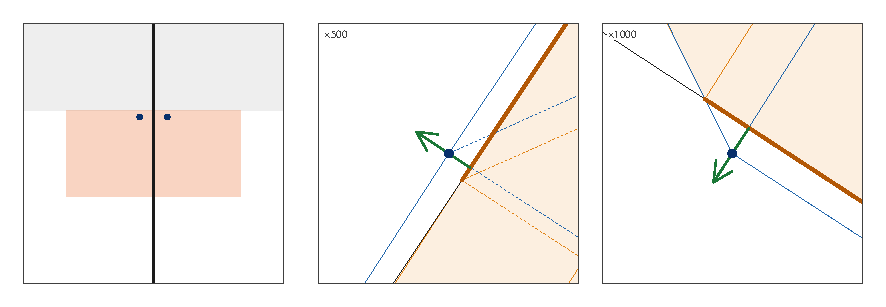
\includegraphics[width=\linewidth]{figures/pentagon-support}
\caption{The two sides of the edge-on line near the pentagon configuration. Left: the pentagon cover's viewing parameters in the coordinates $(\eta,\xi)$, with $\eta\in[-3/64,3/64]$ horizontally and $\xi\in[-1/16,1/32]$ vertically: \fc{Pentagon}{the covered rectangle $|\eta|\le1/32$, $-1/32\le\xi\le0$ (red-orange)}, \fc{Grey}{the views beyond the viewing triangle, $\xi>0$ (grey)}, the edge-on line $\eta=0$ (black) and two examples (dots) at $(\eta,\xi)=(-1/200,-1/400)$ and $(1/200,-1/400)$, both with the rotation $\mathbf r=(1/1000,0,0)$. Middle and right: their shadows near the protruding plug vertex, enlarged $500$ and $1000$ times, with the \fc{Hole}{hole (orange)} and the \fc{Plug}{plug (blue)} as in \cref{fig:global-examples} and a supporting line of the hole's shadow that \fc{Vertex}{this vertex (dark blue dot)} lies beyond. On the two sides, different plug vertices protrude beyond different hole edges.}
\label{fig:pentagon-support}
\end{figure}

\begin{proposition}[The pentagon neighbourhood]\label{prop:pentagon-neighbourhood}
  Every configuration $c\in D$ with $|\eta|\le1/32$, $-1/32\le\xi\le0$ and
  $\lVert\mathbf r\rVert_\infty\le1/16$ is a touch configuration if
  $\mathbf r=\mathbf0$ and a poke configuration otherwise.
\end{proposition}
\begin{proof}
  As for \cref{prop:square-neighbourhood}, using \cref{lem:point-coverage}
  and \cref{lem:zoom-lemma}; every cell's witness is a gap polynomial.
\end{proof}

\subsection{A neighbourhood of all aligned configurations}\label{subsec:ranges-and-remaining-touch-configurations}

The square and pentagon covers, together with the 30 covers of the Local
component, give a uniform neighbourhood of all aligned representatives.
Recall that a configuration lies in the range of the collection when the
collection accepts every search box in some neighbourhood of it
(\cref{def:range-of-a-component}). Write $\Delta$ for the viewing triangle
\cref{eq:viewing-triangle}, $W_0=[0,2/3]\times[0,2/5]$ for the viewing
rectangle of $B_0$, and $\delta_0=1/200$ for the smallest rotation bound
among the 32 covers of aligned configurations. Each of these covers has a
set of viewing parameters: a rectangle, or, for the pentagon cover, the
half-strip $|\eta|\le1/32$, $\xi\ge-1/32$ of its acceptance test (the upper
bound on $\xi$ is dropped because configurations with $\xi>0$ lie outside
$D$). Each cover contains every configuration whose viewing parameters lie
in its set and whose rotation satisfies
$\lVert\mathbf r\rVert_\infty\le\delta_0$. Shrink each set by $\beta=1/4096$ in
the maximum norm, except along the sides of $W_0$ (the half-strip has no
upper side to shrink). An
exact computation, bisecting $W_0$ and comparing endpoints in
$\mathbb Q(\sqrt5)$, shows that the shrunk sets still cover $\Delta$; without
the margin of $1/1024$ around each Local rectangle, which makes neighbouring rectangles overlap, this would
fail.

\begin{proposition}[A neighbourhood of all aligned representatives]\label{prop:aligned-neighbourhood}
  For every $(s_0,t_0)\in\Delta$, some cover of aligned configurations contains
  every configuration $[s,t,\mathbf r]\in B_0$ with
  $\max\{|s-s_0|,|t-t_0|\}\le\beta$ and $\lVert\mathbf r\rVert_\infty\le\delta_0$. Every
  such configuration in $D$ is a touch configuration when $\mathbf r=\mathbf0$ and a
  poke configuration otherwise. In particular, the union
  \begin{equation}\label{eq:aligned-neighbourhood-range}
    \bigcup_{(s_0,t_0)\in\Delta}\bigl\{[s,t,\mathbf r]\in B_0:
      \max\{|s-s_0|,|t-t_0|\}<\beta,\ \lVert\mathbf r\rVert_\infty<\delta_0\bigr\}
  \end{equation}
  lies in the collection's range.
\end{proposition}
\begin{proof}
  The pair $(s_0,t_0)$ lies in the shrunk set of some cover, so the
  maximum-norm ball of radius $\beta$ around it, cut to $W_0$, lies in that
  cover's set of viewing parameters. The geometric claim follows from
  \cref{prop:soundness-of-the-local-component,prop:square-neighbourhood,prop:pentagon-neighbourhood}.

  For the range, let $c$ lie in the union \cref{eq:aligned-neighbourhood-range}.
  It has a neighbourhood in $B_0$ inside one of the closed sets just
  described, and hence inside the covered set of one cover. Every search
  box contained in that neighbourhood lies in the covered set, so the
  cover's exact inclusion test accepts it.
\end{proof}

Because of the overlaps, the conclusion does not depend on where the
boundaries of the covers lie relative to the halving lines of the search,
and every aligned representative lies in the range, even on a boundary of
the viewing triangle.

\paragraph{Remaining touch configurations.}
With the Global and Local components and these two covers, the
unresolved boxes no longer concentrate around aligned configurations.
They concentrate instead along two segments of configurations in which the
plug and the hole have different orientations but their shadows still
touch (\cref{fig:arcs-remaining}). We describe them and the covers along
them in \cref{sec:arc-configurations}.

\begin{figure}[htbp]
\centering
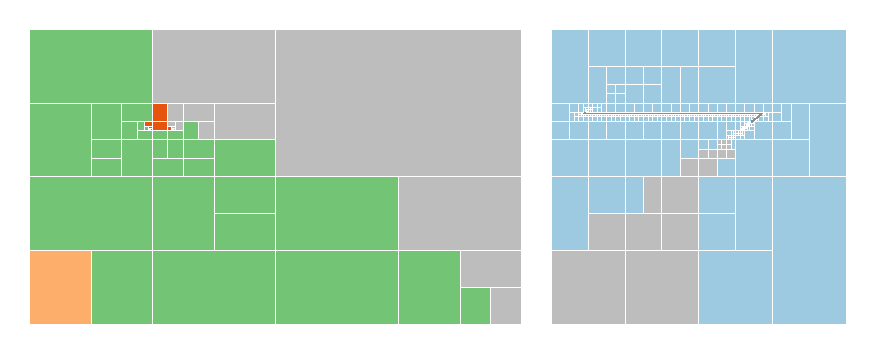
\includegraphics[width=\linewidth]{figures/arcs-remaining}
\caption{With the square and pentagon covers added. Left: the plane $\mathbf r=\mathbf 0$ of \cref{fig:exotic-directions}, now eliminated entirely, near the corner by \fc{Square}{the square cover (light orange)} and near the edge-on point by \fc{Pentagon}{the pentagon cover (red-orange)}. Right: a plane of non-aligned configurations with $t=0$, with $s\in[3/16,5/8]$ horizontally and a rotation parameter $\theta\in[-5/16,1/8]$ vertically (it is the plane $\Pi_1$ of \cref{sec:arc-configurations}). Unresolved pieces (black) remain along two segments that meet at $s=1/2$.}
\label{fig:arcs-remaining}
\end{figure}

% !TEX root = ../main.tex
\pagebreak[0]
\section{\emph{Arc} configurations}\label{sec:arc-configurations}

\begin{figure}[htbp]
\centering
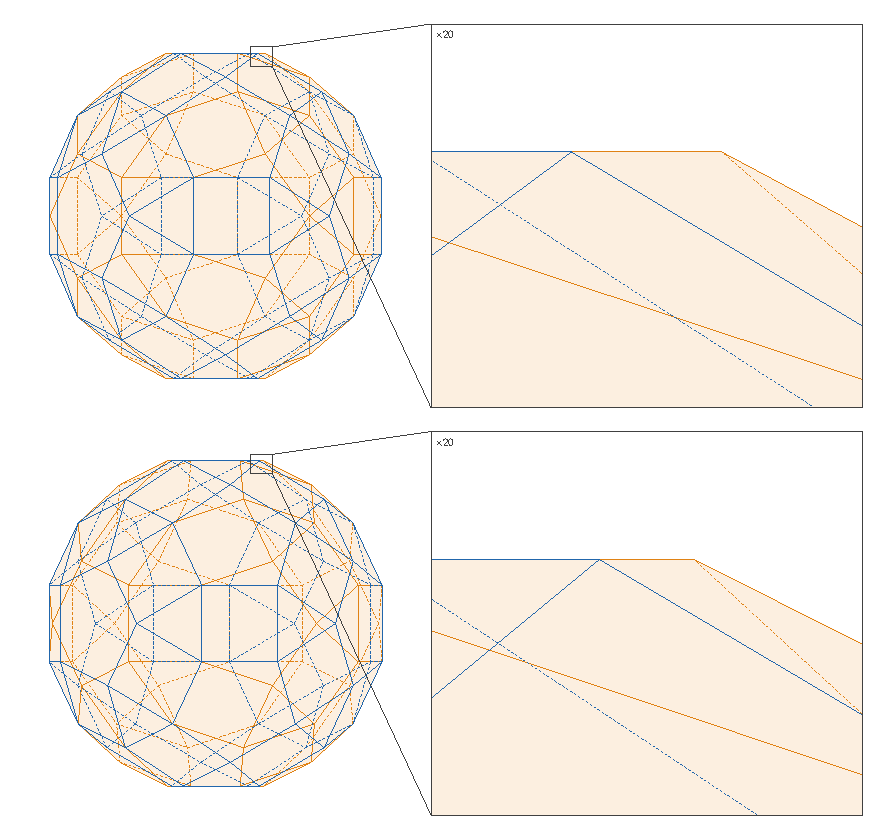
\includegraphics[width=\linewidth]{figures/arcs}
\caption{Two touch configurations on the first arc of the plane $\Pi_1$, at $e=1/10$ and $e=3/20$ ($t=0$, $\theta=0$); the \fc{Hole}{hole (orange)} and the \fc{Plug}{plug (blue)} as in \cref{fig:global-examples}. Both shadows reach exactly as far in the upward screen direction, which is $\mathbf e_2$, and share their top edge. The enlargements, $20$ times at the right ends of the two top edges, show the plug's top edge ending inside the hole's.}
\label{fig:arc-examples}
\end{figure}

The boxes left unresolved by the preceding components cluster around
configurations with $t=0$, a range of values of $s$, and a relative
rotation close to a turn through $36^\circ$ about a five-fold axis of the
RID, followed by a small turn about the second coordinate axis. For $t=0$,
that axis lies in the shadow plane, and a turn about it does not change
how far the plug reaches in its direction. The $36^\circ$ turn happens to
leave that reach equal to the hole's, so whatever the second turn, the
plug's shadow reaches exactly as far as the hole's in that direction, and
none of these configurations is a fit. This gives two planes of configurations, each a
no-fit set for a reason as simple as for the aligned configurations. Around
the touch configurations in them, the Exotic component uses tube
zooms that divide out the distance from such a plane, much as the Local
component divides out the size of the rotation.

\subsection{Geometry of \emph{non-aligned touch} configurations}\label{subsec:geometry-of-non-aligned-touch-configurations}

\paragraph{The arc planes.}
Let
\[
  a_1=\frac{-5+3\sqrt5}{10},\qquad a_3=\frac{-5+\sqrt5}{10},\qquad
  \mathbf r_A=(a_1,0,a_3),
\]
and, for $\sigma\in\{-1,1\}$, $\mathbf w_\sigma=(\sigma a_3,1,-\sigma a_1)$.
The two \emph{arc planes} are the families of configurations
\begin{equation}\label{eq:arc-plane}
  \Pi_\sigma=\bigl\{[s,0,\sigma\mathbf r_A+\theta\mathbf w_\sigma]:\ s,\theta\in\mathbb R\bigr\},
  \qquad \sigma\in\{-1,1\},
\end{equation}
two-dimensional sets of configurations with $t=0$. Since
$\lVert\mathbf r_A\rVert=\tan18^\circ$, the rotation $R_P(\mathbf r_A)$ is a turn
through $36^\circ$ about the axis of $\mathbf r_A$, which is a five-fold axis
of the RID; its square is a symmetry of $\mathcal R$, but it is not one
itself. With $\mathbf e_2=(0,1,0)$, the quaternion product gives
\[
  (1,\theta\mathbf e_2)(1,\sigma\mathbf r_A)
  =(1-\theta\sigma\,\mathbf e_2\cdot\mathbf r_A,\ \theta\mathbf e_2+\sigma\mathbf r_A
     +\theta\sigma\,\mathbf e_2\times\mathbf r_A)
  =(1,\sigma\mathbf r_A+\theta\mathbf w_\sigma),
\]
because the second coordinate of $\mathbf r_A$ is zero. Hence
$R_P(\sigma\mathbf r_A+\theta\mathbf w_\sigma)=R_P(\theta\mathbf e_2)R_P(\sigma\mathbf r_A)$:
the plug is first turned through $36^\circ$ and then through the angle
$2\arctan\theta$ about the second coordinate axis.

\begin{lemma}[The arc planes contain no fit]\label{lem:arc-planes-contain-no-fit}
  No configuration in $\Pi_{1}$ or $\Pi_{-1}$ is a fit.
\end{lemma}
\begin{proof}
  On $\Pi_\sigma$ we have $t=0$, so $\mathbf e_2$ is perpendicular to
  $\mathbf u=(s,0,1)$: it is a direction in the shadow plane, and
  $\mathbf e_2\cdot\mathbf x$ is unchanged by projection. A turn about the
  second coordinate axis does not change $\mathbf e_2\cdot\mathbf x$ either.
  So the plug's support value in the direction $\mathbf e_2$ is
  \[
    \max_{\mathbf v\in V}\mathbf e_2\cdot R_P(\sigma\mathbf r_A)\mathbf v
     =2+\sqrt5=\max_{\mathbf v\in V}\mathbf e_2\cdot\mathbf v,
  \]
  the hole's support value; the middle equality is an exact comparison over
  the sixty vertices of \cref{eq:rhombicosidodecahedron-vertices}. A fit
  places the compact plug shadow in the interior of the hole shadow, which
  requires a strictly smaller support value in every direction of the
  shadow plane.
\end{proof}

The two planes describe the same plug positions, since
$R_P(\mathbf r_A)^2$ is a symmetry of the plug, but they are different
subsets of $B_0$. Both lie in the hyperplanes on which the following
inequalities hold with equality, so their configurations in $D$ lie on the
boundary of $D$: on $\Pi_\sigma$, the
relative-rotation comparison
\begin{equation}\label{eq:tie-inequality}
  \sigma\bigl(\varphi^{-1}r_1-r_3\bigr)\le2-\varphi
\end{equation}
of \cref{eq:reduced-domain} (the one with $i=3$, $\epsilon=-\sigma$ and
$\delta=\sigma$) holds with equality, because
$\varphi^{-1}a_1-a_3=2-\varphi$ and $a_1+\varphi^{-1}a_3=0$. Along the plane,
two representatives of the same configuration tie, and the comparison
decides between them; we call \cref{eq:tie-inequality} the \emph{tie
inequality} of $\Pi_\sigma$. Every construction below comes in two copies,
one for each sign $\sigma$; the map $(r_1,r_2,r_3)\mapsto(-r_1,r_2,-r_3)$
exchanges the two planes, keeping $s$ and $\theta$, together with their tie
inequalities.

\paragraph{Arc coordinates.}
Near $\Pi_\sigma$ we use the coordinates
\begin{equation}\label{eq:arc-coordinates}
  e=\frac{1-2s}{2+s},\quad v=\frac{5t}{2+s},\quad \theta=r_2,\quad
  \zeta_1=r_1-\sigma(a_1+a_3\theta),\quad
  \zeta_3=r_3-\sigma(a_3-a_1\theta),
\end{equation}
defined for $s>-2$. Then
\[
  \mathbf u=(1-2e,\ v,\ 2+e)=\frac5{2+s}(s,t,1),\qquad
  \mathbf r=\sigma\mathbf r_A+\theta\mathbf w_\sigma+(\zeta_1,0,\zeta_3),
\]
so $\mathbf u$ is a positive multiple of $(s,t,1)$ with components affine
in $e$ and $v$, as zooms require, and every witness is again a polynomial
in the new coordinates. The plane $\Pi_\sigma$ is $v=\zeta_1=\zeta_3=0$. The
coordinate $e$ is chosen so that both families of touch configurations
below are straight lines in the plane, crossing at $e=0$; this matters for
the shear in \cref{subsec:eliminating-the-crossing-configuration}.

\paragraph{The arcs.}
Inside each plane lie two segments of touch configurations
(\cref{fig:arc-examples,fig:endpoint-crossing-examples}):
\begin{itemize}
  \item the \emph{first arc}, $\theta=0$ with $0\le e\le e_*=\sqrt5-2$, that is
    $s\in[\sqrt5-2,1/2]$;
  \item the \emph{second arc}, $\theta=-e$ with $0\le e\le e_*$.
\end{itemize}
Along the first arc, the two shadows share their top edge in the direction
$\mathbf e_2$, the plug's top edge ends inside the hole's, and the rest of
the plug's shadow lies inside the hole's. At the \emph{endpoint} $e=e_*$, the
ends of the two top edges coincide; beyond it, the plug's top edge is the
longer one, and its corner pokes out. The two arcs meet at the
\emph{crossing}, $e=0$, where $s=1/2$. Elsewhere in the plane, the
configurations are poke configurations, and the Global component handles
them (\cref{fig:arc-plane-slice}). These properties explain where zooms are
needed; the proof itself uses only \cref{lem:arc-planes-contain-no-fit}.

The second arc lies outside $D$ except at the crossing. On it, the
polynomial of one of the fold inequalities of \cref{eq:reduced-domain},
written homogeneously in the viewing vector $(1-2e,v,2+e)$, equals
$5e^2+5e^4$, which is positive for $e>0$. Sufficiently small boxes around
its configurations with $e>0$ are therefore eliminated by the Domain
component, and no cover follows the second arc; near the crossing it is
handled in \cref{sec:endpoint-and-crossing-configurations}.

\begin{figure}[htbp]
\centering
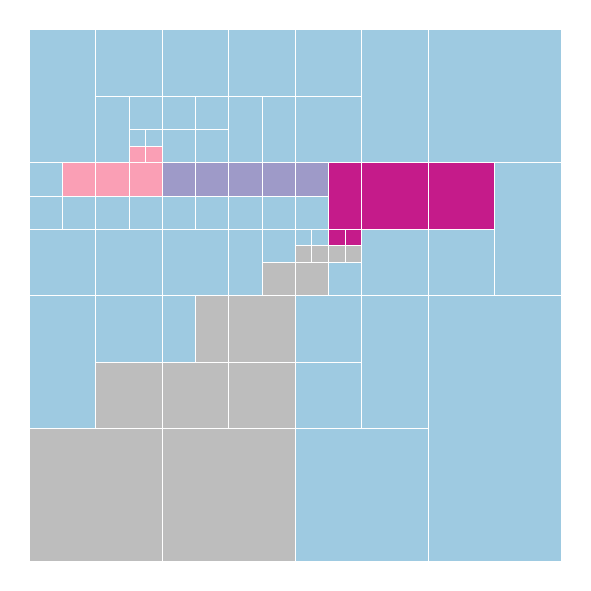
\includegraphics[width=0.55\linewidth]{figures/slice-arcs}
\caption{A slice of the final collection through the plane $\Pi_1$: horizontally $s\in[3/16,5/8]$, vertically $\theta\in[-5/16,1/8]$ (with $\mathbf r_A$ rounded to rationals within $10^{-14}$), halved alternately until one component eliminates each piece, which is coloured by that component: \fc{Global}{light blue Global}, \fc{Domain}{grey Domain}, \fc{Arc}{lavender the arc cover}, \fc{Endpoint}{light pink the endpoint cover} (near $s=\sqrt5-2$) and \fc{Crossing}{magenta the crossing cover} (near $s=1/2$). The first arc is the segment $\theta=0$ between these two values. The Global component handles the configurations of the plane away from the arcs, and the Domain component the pieces outside $D$, including those along the second arc away from the crossing.}
\label{fig:arc-plane-slice}
\end{figure}

\subsection{Eliminating \emph{arc} configurations}\label{subsec:eliminating-arc-configurations}

Along the first arc, a small displacement off the plane $\Pi_\sigma$ moves
some projected plug vertex beyond the hole shadow at a rate proportional to
the displacement. This is the situation of the aligned configurations, and
the tube zooms of \cref{subsec:the-zoom-lemma} apply.

\paragraph{The arc covers.}
Along the first arc of $\Pi_\sigma$, the base coordinate is $e$ and the
offset coordinates are $(v/2,\theta,\zeta_1,\zeta_3)$, weighting $v$ by one
half. The offset box is $\Phi=[0,1]\times{[-1,1]}^3$, since $t\ge0$ forces
$v\ge0$. This gives seven tube zooms, with $e\in[3/64,3/16]$ and
$\delta_{\max}=1/32$, so the covered set consists of the configurations with
\[
  \frac3{64}\le e\le\frac3{16},\qquad 0\le v\le\frac1{16},\qquad
  |\theta|,|\zeta_1|,|\zeta_3|\le\frac1{32}.
\]
The no-fit set of the zooms is the plane $\Pi_\sigma$: where $\delta=0$, the
offsets vanish, so the configuration lies on the first arc. The view
$\mathbf u=(1-2e,v,2+e)$ has $u_3=2+e>0$ and components affine in each zoom
coordinate, as \cref{def:zoom} requires. The weight of $v$, the radii and
the range of $e$ are tuning choices: the proof needs only that every cell
passes its check and that the covers overlap as described in
\cref{subsec:the-arcs-together}.

Most cells carry gap polynomials with the zoom factor $\delta$. Part of the
covered set lies on the far side of the tie inequality, outside $D$; there
the tie inequality itself serves as the witness. The cover for $\sigma=1$
has 343 terminal cells, 32 of them with the tie inequality, and the cover
for $\sigma=-1$ has 288, with 72.

\begin{proposition}[The arc neighbourhoods]\label{prop:arc-neighbourhoods}
  For each $\sigma\in\{-1,1\}$, no configuration of $D$ in the covered set
  above is a fit.
\end{proposition}
\begin{proof}
  By \cref{lem:tube-coverage}, such a configuration lies in
  $\Pi_\sigma$, which contains no fit by
  \cref{lem:arc-planes-contain-no-fit}, or in a checked cell. There
  \cref{lem:zoom-lemma} applies to the cell's witness: a gap polynomial
  excludes a fit, and the tie inequality shows that the configuration lies
  outside $D$.
\end{proof}

A search box lies in the covered set exactly when the ranges of the five
arc coordinates over the box lie in the stated intervals. The coordinates
$e$ and $v$ are monotone in $s$ and in $t$ separately, and $\theta$,
$\zeta_1$ and $\zeta_3$ are affine in $\mathbf r$, so each range is attained at
corners of the box and the inclusion test consists of exact comparisons.

\paragraph{Where the arc covers stop.}
The arc covers stop short of both $e=0$ and $e=e_*$. The rate at which a
displacement off the plane moves some projected vertex outward shrinks
linearly towards both ends of the first arc, like $e$ at the crossing and
like $e_*-e$ at the endpoint. At those two points the quotient after
dividing by $\delta$ vanishes in some directions, exactly as at the square
and pentagon configurations, and the unresolved boxes concentrate there
(\cref{fig:arcs-residual}). We treat the endpoint and the crossing with
point zooms in \cref{sec:endpoint-and-crossing-configurations}.

\begin{figure}[htbp]
\centering
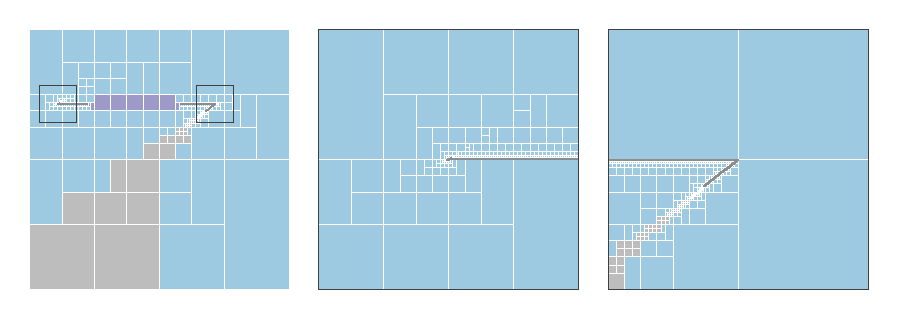
\includegraphics[width=\linewidth]{figures/arcs-residual}
\caption{The plane $\Pi_1$ as in \cref{fig:arc-plane-slice}, halved $18$ times with \fc{Arc}{the arc covers added (lavender)} but not yet the endpoint and crossing covers. Unresolved pieces (black) remain only near the two ends of the first arc. Middle: the window of half-width $1/32$ around the endpoint, $s=\sqrt5-2$, $\theta=0$; right: the same around the crossing, $s=1/2$, $\theta=0$, where the second arc leaves the first. Away from the crossing, the second arc lies outside $D$ \fc{Domain}{(grey)}.}
\label{fig:arcs-residual}
\end{figure}

% !TEX root = ../main.tex
\pagebreak[0]
\section{\emph{Endpoint} and \emph{crossing} configurations}\label{sec:endpoint-and-crossing-configurations}

\begin{figure}[htbp]
\centering
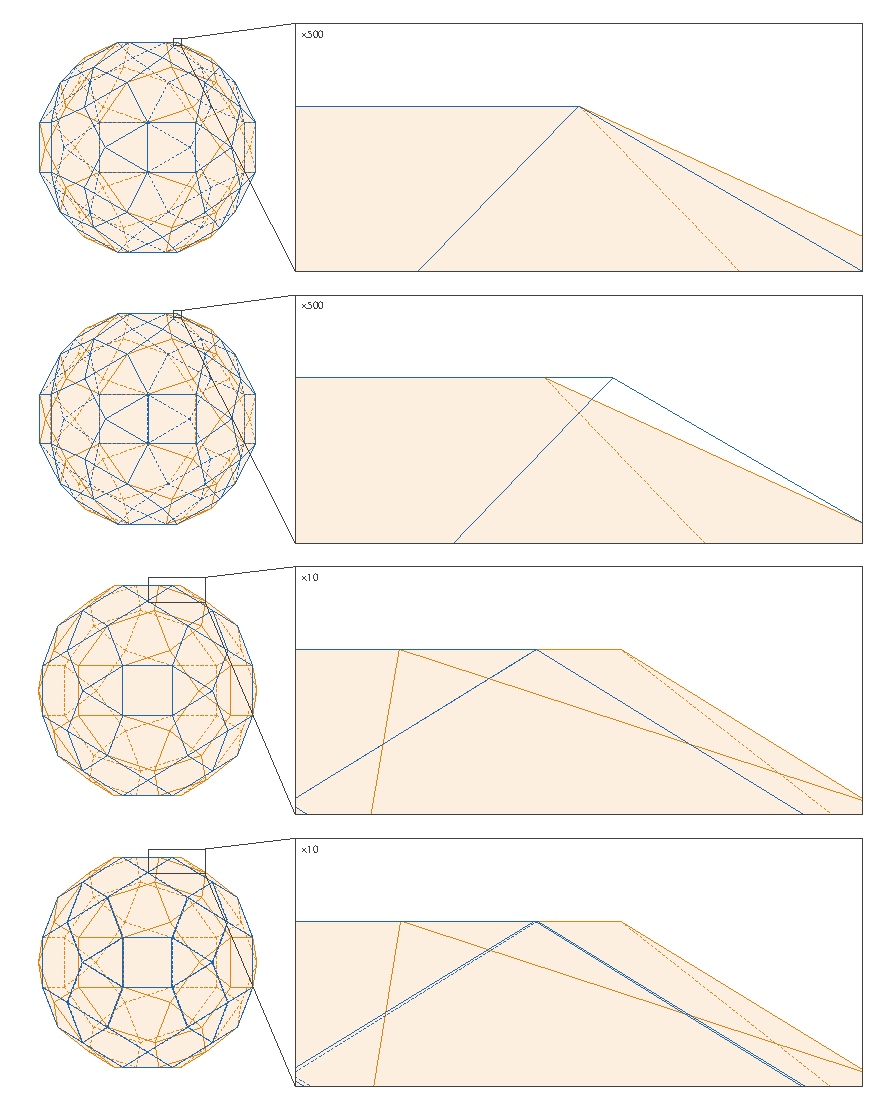
\includegraphics[width=\linewidth]{figures/endpoint-crossing}
\caption{Configurations in the plane $\Pi_1$, enlarged at the right ends of the two top edges as in \cref{fig:arc-examples}, $500$ times for the first two and $10$ times for the last two; the \fc{Hole}{hole (orange)} and the \fc{Plug}{plug (blue)} as in \cref{fig:global-examples}. First: the endpoint $e=e_*$, where the ends of the two top edges coincide. Second: $e=e_*+1/256$ on the continuation of the first arc, where the plug's top edge is longer than the hole's and its corner protrudes, a poke configuration. Third: the crossing $e=0$. Fourth: the configuration $e=1/200$, $\theta=-1/200$ of the second arc, which lies outside $D$.}
\label{fig:endpoint-crossing-examples}
\end{figure}

At the two ends of the first arc, the rate of outward motion off the arc
plane shrinks to zero, as it did at the square and pentagon
configurations. The remedy is the same: point zooms that divide out two
distances, the distance along the arc from the special configuration and
the displacement off the arc measured relative to it. The crossing needs
one further idea, because the second arc passes through it.

Both covers use the arc coordinates \cref{eq:arc-coordinates} of one plane
$\Pi_\sigma$ and come in two copies, one for each sign $\sigma$. Their base
coordinate is $e$ measured from the special configuration, and their offset
coordinates are those of the arc covers, with $v$ weighted.

\subsection{Eliminating the \emph{endpoint} configuration}\label{subsec:eliminating-the-endpoint-configuration}

At the endpoint $e=e_*$, the first arc ends: beyond it, the configurations
of the plane poke. Around it we use a point zoom cover as in
\cref{sec:square-and-pentagon-configurations}, with base coordinate
$e-e_*$ and $\Sigma=[-1,1]$, offset coordinates $(v/2,\theta,\zeta_1,\zeta_3)$
with $\Phi=[0,1]\times{[-1,1]}^3$, and ratio $\rho_0=1$. The base radius is
$1/16$ on the face $e<e_*$ and $1/32$ on the face $e>e_*$, and the offset
radius is $\delta_{\max}=1/32$. The two base faces and seven offset faces
give 14 zooms in family A and seven in family B. The covered set consists
of the configurations with
\[
  -\frac1{16}\le e-e_*\le\frac1{32},\qquad 0\le v\le\frac1{16},\qquad
  |\theta|,|\zeta_1|,|\zeta_3|\le\frac1{32}.
\]
The no-fit set of the zooms is the plane $\Pi_\sigma$, by
\cref{lem:arc-planes-contain-no-fit}.
As at the square configuration, some directions of displacement move no
projected vertex outward at first order at the endpoint itself, and the
cells there use two kinds of witnesses: one whose limit after division
contains the base coordinate, and a radial one.

\begin{proposition}[The endpoint neighbourhoods]\label{prop:endpoint-neighbourhoods}
  For each $\sigma\in\{-1,1\}$, no configuration of $D$ in the covered set
  above is a fit.
\end{proposition}
\begin{proof}
  As for \cref{prop:arc-neighbourhoods}, with \cref{lem:point-coverage}
  in place of \cref{lem:tube-coverage}.
\end{proof}

\subsection{Eliminating the \emph{crossing} configuration}\label{subsec:eliminating-the-crossing-configuration}

At the crossing $e=0$, the second arc $\theta=-e$ meets the first. The point
zoom cover around it has base coordinate $e$ with $\Sigma=[-1,1]$, offset
coordinates $(4v/5,\theta,\zeta_1,\zeta_3)$ with $\Phi=[0,1]\times{[-1,1]}^3$,
radii $\mu_{\max}=\delta_{\max}=1/16$ and ratio $\rho_0=5/4$: 14 zooms in
family A and seven in family B, with the covered set
\[
  |e|\le\frac1{16},\qquad 0\le v\le\frac5{64},\qquad
  |\theta|,|\zeta_1|,|\zeta_3|\le\frac1{16}.
\]
The distance coordinates of these zooms vanish only on the segment
$\theta=0$, $|e|\le1/16$ of $\Pi_\sigma$, which contains the first arc near
the crossing; the no-fit set of the zooms is $\Pi_\sigma$, by
\cref{lem:arc-planes-contain-no-fit}. The second arc, however, is also a
family of touch configurations, and it runs through the domain of one
zoom. In the family A zoom on the base face
$e=\mu>0$ and the offset face $\theta=-1$, the second arc is the set where
$\rho=1$ and the other offset coordinates vanish. No gap polynomial is
positive at a touch configuration. The fold inequality is violated on the
second arc for $e>0$ (\cref{sec:arc-configurations}), but at the crossing its
polynomial has first-order terms in $v$, $\zeta_1$ and $\zeta_3$: in this zoom
it is divisible only by $\mu$, and its quotient at $\mu=0$ is $\rho$ times a
linear form in the off-plane offsets, which vanishes on the second arc. So
no cell containing the end $\mu=0$ of the second arc can pass the test. Whatever the ratio, the second arc meets some zoom domain;
with $\rho_0=5/4>1$ it lies inside family A only, away from the boundary
$\rho=\rho_0$ between the two families, and only cells of family A need
the following treatment.

\paragraph{Handing cells over.}
The cells of family A along the second arc are covered by other zooms,
built in the same way around the second arc instead of the first. The
\emph{sheared} offset $\theta'=\theta+e$ measures the displacement from the
second arc. The sheared zooms $\mathcal A'_{G,F}$, for the base face $G$
with $e>0$ and every offset face $F$, are the zooms of family A with
$\theta'$ in place of $\theta$ and the ratio $\rho'\in[0,\rho_0']$,
$\rho_0'=1/4$. Their distance coordinates vanish only on the second arc,
which lies in the no-fit plane $\Pi_\sigma$. A cell of family A whose
configurations, measured from the second arc, stay within the domains of
the sheared zooms needs no witness of its own: it is \emph{handed over},
and the checked cells of the sheared zooms take its place.

To state this precisely, let $\mathcal A_{G,F}$ be a zoom of family A on
the base face $G$ with $e>0$, so that $e=\mu$, and write
\[
  \mathbf o(\mathbf y)=\rho\widehat{\mathbf f}+(0,1,0,0)
\]
for the offset measured from the second arc in units of $\mu$: the shear
adds $e=\mu$ to the second offset coordinate $\theta$.

\begin{lemma}[Hand-over]\label{lem:hand-over}
  Let $C$ be a cell of a zoom $\mathcal A_{G,F}$ of family A, on the base
  face $G$ with $e>0$, such that $\mathbf o(\mathbf y)\in\rho_0'\Phi$ for every
  $\mathbf y\in C$. Then every configuration in the image of $C$ lies in the
  no-fit set or is the image of a point in the domain of one of the sheared
  zooms $\mathcal A'_{G,F'}$.
\end{lemma}
\begin{proof}
  At $\mathbf y\in C$, the base coordinate is $\mu$ and the sheared offset
  is $\mu\,\mathbf o(\mathbf y)$. If $\mathbf o(\mathbf y)=\mathbf0$, the
  configuration lies on the second arc, in the no-fit set. Otherwise
  $\rho'=\lVert\mathbf o(\mathbf y)\rVert_\infty\in(0,\rho_0']$, and
  $\widehat{\mathbf f}'=\mathbf o(\mathbf y)/\rho'$ lies on a face $F'$ of $\Phi$,
  giving a point of the domain of $\mathcal A'_{G,F'}$ with the same
  configuration.
\end{proof}

The hypothesis is checked exactly for each handed-over cell: each
coordinate of $\mathbf o$ is the product of two zoom coordinates, plus a
constant for the second, so its exact range over the cell follows from
interval products. Cells are handed over only from family A to the sheared
family, never back. The cover for $\sigma=1$ hands 34 cells over, and the
cover for $\sigma=-1$ hands over 14 (\cref{fig:crossing-plane}).

\begin{figure}[htbp]
\centering
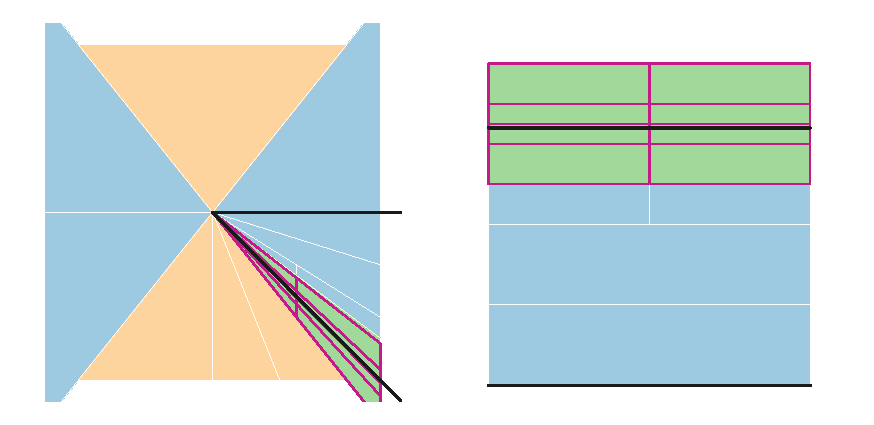
\includegraphics[width=\linewidth]{figures/crossing-plane}
\caption{The crossing cover of $\Pi_1$ where it meets the plane itself ($v=\zeta_1=\zeta_3=0$). Left: in the coordinates $(e,\theta)$, both in $[-9/128,9/128]$, the cells of \fc{Global}{family A (light blue}; $|\theta|\le\tfrac54|e|$, cut by rays of constant ratio), of \fc{FamilyB}{family B (light orange}; $|e|\le\tfrac45|\theta|$) and of \fc{Sheared}{the sheared zooms around the second arc (green)}; \fc{Crossing}{the cells of family A handed over to the sheared zooms are outlined in magenta}, and the first arc $\theta=0$ and the second arc $\theta=-e$ are black. Right: the family A zoom on the base face $e=\mu>0$ and the offset face $\theta=-1$, in its own coordinates ($20\mu\in[0,5/4]$ horizontally, $\rho\in[0,5/4]$ vertically), in which the first arc is $\rho=0$ and the second arc $\rho=1$ (black): \fc{Global}{its cells in the plane (light blue)} and, along $\rho=1$, \fc{Sheared}{the cells it hands over (green,} \fc{Crossing}{outlined in magenta}). Most of the refinement of this cover happens in $v$, $\zeta_1$ and $\zeta_3$, so few cells meet the plane.}
\label{fig:crossing-plane}
\end{figure}

\begin{proposition}[The crossing neighbourhoods]\label{prop:crossing-neighbourhoods}
  For each $\sigma\in\{-1,1\}$, no configuration of $D$ in the covered set
  above is a fit.
\end{proposition}
\begin{proof}
  By \cref{lem:point-coverage}, a configuration of the covered set lies in
  the no-fit set $\Pi_\sigma$, in a checked cell with a witness, or in a
  handed-over cell.
  The first two cases are as for \cref{prop:arc-neighbourhoods}. In the
  third, \cref{lem:hand-over} places the configuration on the second arc
  or in the domain of a sheared zoom, whose cells are checked by
  \cref{lem:zoom-lemma}.
\end{proof}

\subsection{The arcs together}\label{subsec:the-arcs-together}

The covers along the first arc overlap: the arc cover and the crossing
cover share $3/64\le e\le1/16$, and the arc cover and the endpoint cover
share $e_*-1/16\le e\le3/16$. Every configuration of the first arc with
$0\le e\le e_*$ therefore lies in the interior, relative to $B_0$, of the
covered set of one cover, and so in the collection's range. The second arc
lies outside $D$ for $e>0$ and meets the crossing cover at $e=0$. Together
with \cref{prop:aligned-neighbourhood}, the collection's range contains a
neighbourhood of every touch configuration of $D$ that the subdivision
revealed. That the collection eliminates every box is confirmed by the
search itself, in \cref{sec:generating-and-verifying-the-certificate}.

% !TEX root = ../main.tex
\pagebreak[0]
\section{Generating and verifying the certificate}\label{sec:generating-and-verifying-the-certificate}

The components of the preceding sections are combined in a single search
over $B_0$. Its result is a certificate: one record for every eliminated
box. The certificate is checked separately from the search that produced
it, and this check, together with the mathematics of the preceding
sections, proves \cref{thm:main}.

\subsection{Complete coverage and the main theorem}\label{subsec:complete-coverage-and-the-main-theorem}

\paragraph{The collection.}
The final collection has four components: the Domain component of
\cref{subsec:domain-component-skipping-boxes-outside-the-reduced-domain},
the Global component of \cref{sec:global-component}, the Local component of
\cref{sec:local-component}, and the Exotic component with the eight
covers of \cref{sec:square-and-pentagon-configurations,sec:arc-configurations,sec:endpoint-and-crossing-configurations}.
\Cref{tab:covers} lists the 38 zoom covers. The Local and Exotic
components work in the same way, by inclusion in a checked cover; we keep
them apart because the Local covers form one uniform family, indexed by
viewing rectangles, while each Exotic cover belongs to a particular
configuration. The components are tried in the order Domain, Exotic,
Local, Global, since the first three tests are fast and the Global
component's test is the most expensive.

\begin{table}[htbp]
\centering\small
\begin{tabular}{llllrr}
  \toprule
  Cover & No-fit set & Zooms & Section & Zoom cells & Records\\
  \midrule
  Local $0,\dots,29$ & aligned & tube (face zooms) & \ref{subsec:face-zooms-and-the-local-component} & 833 & 21{,}792\\
  square & aligned & point & \ref{subsec:eliminating-the-square-configuration} & 877 & 56\\
  pentagon & aligned & point & \ref{subsec:eliminating-the-pentagon-configuration} & 6{,}173 & 315\\
  arc$\pm$ & $\Pi_{\pm1}$ & tube & \ref{subsec:eliminating-arc-configurations} & 343, 288 & 135, 68\\
  endpoint$\pm$ & $\Pi_{\pm1}$ & point & \ref{subsec:eliminating-the-endpoint-configuration} & 305, 246 & 55, 23\\
  crossing$\pm$ & $\Pi_{\pm1}$ & point, hand-over & \ref{subsec:eliminating-the-crossing-configuration} & 1{,}431, 687 & 86, 58\\
  \bottomrule
\end{tabular}
\caption{The zoom covers of the Local component (first row) and of the
Exotic component, with the number of their terminal cells that carry
witnesses and the number of certificate records naming them. The pairs are
for $\sigma=1$ and $\sigma=-1$. The parameters of every cover are listed in
\cref{app:zoom-covers}.}
\label{tab:covers}
\end{table}

\paragraph{Records.}
A search box is named by its \emph{path}: the sequence of choices, $0$ for the
lower half and $1$ for the upper half, that leads to it from $B_0$ under the
cyclic bisection of \cref{subsec:boxes-subdivision-and-elimination}. A
certificate record consists of the path, the component that eliminated the
box, and the data its test needs: the violated inequality of $D$ for the
Domain component, the hole edge and plug vertex for the Global component,
and the zoom cover containing the box for the Local and Exotic
components. For example, the record with path \texttt{11} names the
viewing-triangle inequality: the box
$[1/3,2/3]\times[1/5,2/5]\times{[-2/5,2/5]}^3$ lies beyond the boundary
$\varphi s+\varphi^2t=1$.

\paragraph{Checking a certificate.}
A certificate is accepted when two checks succeed.
\begin{enumerate}
  \item \emph{Coverage.} The paths must be the leaves of a finite binary
    tree rooted at $B_0$: no path is a prefix of another, and every
    sequence of choices meets one of them after finitely many steps. The
    checker verifies this by reading the paths in order of increasing depth
    and, within a depth, in lexicographic order, while maintaining the list
    of boxes not yet accounted for; the list must be empty at the end.
  \item \emph{Records.} Each record's test is repeated exactly on its box:
    the Bernstein sign test of the named inequality, the Bernstein sign
    tests of the sixty gap polynomials, or the exact inclusion in the named
    cover's covered set. The covers themselves are rebuilt and all their
    cells checked, as described in \cref{app:zoom-covers}, before any
    record is read.
\end{enumerate}

\begin{proposition}[Complete coverage]\label{prop:complete-coverage}
  If both checks succeed, the boxes of the records cover $B_0$, and every
  box satisfies \cref{eq:box-elimination}.
\end{proposition}
\begin{proof}
  The children of a box cover it, so by induction on the tree, its leaves
  cover the root $B_0$. Each record passed its component's test, and the
  components are sound: the Domain component by
  \cref{subsec:domain-component-skipping-boxes-outside-the-reduced-domain},
  the Global component by \cref{prop:soundness-of-the-global-component},
  the Local component by \cref{prop:soundness-of-the-local-component}, and
  the Exotic component by
  \cref{prop:square-neighbourhood,prop:pentagon-neighbourhood,prop:arc-neighbourhoods,prop:endpoint-neighbourhoods,prop:crossing-neighbourhoods}.
\end{proof}

\begin{proof}[Proof of \cref{thm:main}]
  The final certificate passes both checks. If the RID were Rupert, a fit
  would exist and, by \cref{prop:representative-coverage}, a fit would lie
  in $D\subseteq B_0$. By \cref{prop:complete-coverage}, it would lie in an
  eliminated box, contradicting \cref{eq:box-elimination}.
\end{proof}

\paragraph{What the proof rests on.}
Unwinding the propositions cited above, the proof uses:
\begin{itemize}
  \item the reduction to the domain $D$: \cref{sec:geometric-formulation}
    and \cref{prop:representative-coverage}, with the symmetry data of
    \cref{app:symmetry-data-and-checks};
  \item the Bernstein sign test (\cref{lem:bernstein-sign-test}) and the
    exact arithmetic of \cref{sec:reduction-to-exact-arithmetic};
  \item the Domain and Global tests
    (\cref{subsec:domain-component-skipping-boxes-outside-the-reduced-domain,prop:soundness-of-the-global-component});
  \item the zoom lemma (\cref{lem:zoom-lemma}) with its two kinds of
    witnesses, gap polynomials and domain polynomials;
  \item the two no-fit sets: the aligned configurations
    (\cref{subsec:the-zoom-lemma}) and the arc planes
    (\cref{lem:arc-planes-contain-no-fit});
  \item the coverage lemmas for tube zooms, point zooms and the hand-over
    (\cref{lem:tube-coverage,lem:point-coverage,lem:hand-over}), which give
    the neighbourhood propositions of
    \cref{sec:local-component,sec:square-and-pentagon-configurations,sec:arc-configurations,sec:endpoint-and-crossing-configurations};
  \item a correct implementation of the two checks above, for which the
    independent checker described below provides a second implementation,
    and of the cover checks of \cref{app:zoom-covers}, which that checker
    takes as given and which the program's tests re-verify with independent
    reimplementations.
\end{itemize}
The list of touch configurations, the analyses of why finitely many cells
suffice, the floating-point proposals and the program that found the cells
are not needed.

\subsection{Implementation, execution, and reproducibility}\label{subsec:implementation-execution-and-reproducibility}

The search and the checker form one program, written in Rust, which
combines the performance needed for a search over hundreds of thousands of
boxes with a type system that keeps exact numbers, polynomials, boxes and
records strictly apart. Arbitrarily large integers and rationals come from
the standard \texttt{num} libraries; numbers of $\mathbb Q(\sqrt5)$,
polynomials in five variables and their Bernstein coefficients are
implemented in the program itself, as described in
\cref{sec:reduction-to-exact-arithmetic}. Floating point is used only to
choose which witness to try; every acceptance is decided exactly. The
search processes boxes in a fixed order, so its certificate does not depend
on the number of threads, and it can be interrupted and resumed from the
certificate alone.

The final search, on 16 threads of a workstation, evaluated 385,391 boxes
and wrote 192,696 records in about a minute; checking them takes about half
a minute. Most records are Global records (157,458); the Local, Domain and
Exotic components account for 21,792, 12,650 and 796.
\cref{fig:aligned-slice} shows how the components share a slice of the
configurations.

\begin{figure}[htbp]
\centering
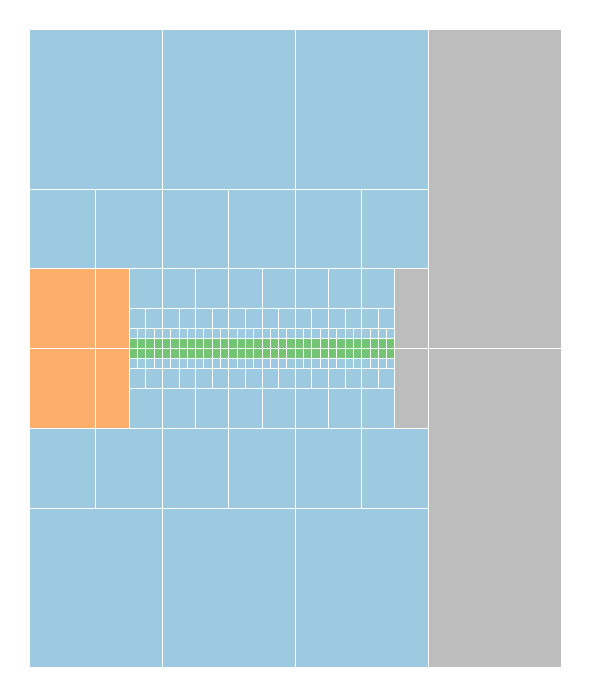
\includegraphics[width=0.5\linewidth]{figures/slice-aligned}
\caption{A slice of the final collection: $t=1/10$ and $r_1=r_2=0$, with $s\in[0,2/3]$ horizontally and $r_3\in[-2/5,2/5]$ vertically, halved alternately until one component eliminates each piece, and coloured by that component: \fc{Global}{light blue Global}, \fc{Local}{green Local}, \fc{Square}{light orange the square cover}, \fc{Domain}{grey Domain} (beyond the boundary of the viewing triangle). The Local component takes over in a thin band around $r_3=0$, where the configurations are nearly aligned. The search itself halves five-dimensional boxes.}
\label{fig:aligned-slice}
\end{figure}

\paragraph{Testing and validation.}
The program is tested extensively, with unit, integration and adversarial
tests of every part, including independent reimplementations of the exact
arithmetic, the zooms and the covers. Two experiments validate the
collection: every configuration of a list of 683 configurations chosen near
the touch configurations of the preceding sections has a neighbourhood
that the collection eliminates, and each component and cover is the only
one to eliminate the boxes around some configuration, so none of them is
redundant. Finally, an independent checker written in Python from the
definitions alone re-verified every record of the final certificate and its
coverage of $B_0$, taking the cells of the zoom covers as checked by the
program.

\paragraph{Reproducibility.}
The program, its zoom cover data, the final certificate and the
independent checker are available in the repository
\url{https://github.com/bence-hervay/nopert-rid}.
From its source directory, building the program
and running its check on the certificate repeats every test of
\cref{subsec:complete-coverage-and-the-main-theorem}; running the search
reproduces the certificate byte for byte. The SHA-256 hash of the final
certificate is
\texttt{df1f8dbab68b561f22fa9daeca48153d}\allowbreak\texttt{71bde7b6fba3345d9f6b7b8077df4b5f}.

% !TEX root = ../main.tex
\pagebreak[0]
\section{Remarks and further directions}\label{sec:remarks-and-further-directions}

\subsection{Relation to previous work}\label{subsec:relation-to-previous-work}

Most of the tools used here are established. Subdividing boxes of
parameters until a sufficient condition holds on each is the classical
branch and bound method. Exact arithmetic in a quadratic field, support
separation of projected vertices, and the centring argument for centrally
symmetric bodies are standard in this context; separation by a supporting
line also underlies the global theorem of
\citet[Section~4, Theorem~17]{SteiningerYurkevichNopertV2}. Bernstein
coefficients as bounds for the range of a multivariate polynomial on a box
go back at least to \citet{Garloff1986}.

Their combination, however, is new in this context. The parametrisation
turns every comparison into a polynomial inequality with coefficients in
$\mathbb Q(\sqrt5)$, so that no trigonometric function has to be bounded
and every step can be checked exactly. Bernstein coefficients then serve as
the single sign test of the whole proof, from the domain inequalities to
the gap polynomials, and the zoom lemma extends that same test to the
neighbourhoods of touch configurations. Together they make the entire
argument a finite list of exact checks, which a certificate records and an
independent program can repeat.

What the RID required, and what we supply, is a way to eliminate the
neighbourhoods of touch configurations, where no strict inequality can
hold and ordinary subdivision cannot finish.
\citet{SteiningerYurkevichNopertV2} proved the Noperthedron Nopert with a
global and a local theorem, and identified an exotic viewing direction
of the RID where their local theorem does not apply; they indicated that its neighbourhood could be treated with
polynomial inequalities, and reported further difficult regions
\citep[Section~9.1]{SteiningerYurkevichNopertV2}. Here the aligned
configurations, the square and pentagon configurations and two
non-aligned families of touch configurations are all treated by one
statement, \cref{lem:zoom-lemma}. The idea is to recognise sets of
configurations that contain no fit for a simple reason, change coordinates
so that some coordinates measure the distance from such a set, and divide
a necessary inequality exactly by a power of those distances before
testing its sign. This is reminiscent of blowing up a singular point in
algebraic geometry, although we use nothing from that theory. The
specific ingredients for the RID are the symmetry-reduced domain with its
fold inequalities, the observation that the non-aligned touch families lie
in planes where the plug reaches exactly as far as the hole in one screen
direction, and the explicit zoom covers of \cref{app:zoom-covers}.
\Cref{thm:main} settles the conjecture of \citet{SteiningerYurkevich2023}
that the RID is not Rupert.

\subsection{Extensions and possible automation}\label{subsec:extensions-and-possible-automation}

\paragraph{What transfers.}
The argument uses few properties of the RID beyond its exact vertex
coordinates, its central symmetry and its symmetry group. For another
centrally symmetric polyhedron with vertex coordinates in a real number
field, the Global component applies unchanged, the Local component applies
in the same form with new covers, and the Domain component needs that
polyhedron's own reduced domain. The Exotic component's covers are
specific to the RID, but their construction is not: each consists of a
no-fit set, an affine change to base and offset coordinates, and the boxes
and radii of a tube or point zoom. Much of the work is already automatic.
The zoom cells and their witnesses were found by a program, the parameters
of each cover amount to a few numbers, and exact arithmetic decides the
equalities on which the no-fit sets rest. The step that required insight
was finding the touch configurations and the no-fit sets containing them.
A natural next step is to apply the method to other polyhedra conjectured
to be Nopert.

\paragraph{Towards a decision procedure.}
We expect these techniques to lead to a practical algorithm that decides
Rupert's property for centrally symmetric polyhedra, once the special cases
can be enumerated algorithmically. The missing ingredient is a finite
procedure that finds, for a given polyhedron, every family of touch
configurations together with a no-fit set containing it, and the points on
these families where a second distance must be divided out. The aligned
configurations are always touch configurations, and the exotic viewing
directions of the Local component might be enumerated: if the component
fails only where faces are seen edge-on, the candidates are finitely many
intersections of great circles on the viewing sphere. Non-aligned touch
families, such as the arcs of \cref{sec:arc-configurations}, need a separate
analysis, and we do not know whether they always lie in no-fit sets as
simple as the arc planes. Given such an enumeration, the remaining steps
are mechanical: placing zoom covers around the families, searching for cells
and witnesses, and running the subdivision with the resulting collection,
which would also detect a fit if one existed
(\cref{subsec:robustly-detecting-potential-rupertness}). We expect this to
be practical for polyhedra whose vertex coordinates are algebraic of low
degree, whose symmetry group is large enough to make the reduced
configuration space small, and which are regular in other respects, as the
RID is; how far it extends is a question for further work.

The checks performed on the certificate are few and elementary, and
together with the lemmas of
\cref{sec:geometric-formulation,sec:symmetry-reduced-domain,sec:reduction-to-exact-arithmetic,sec:global-component,sec:local-component,sec:square-and-pentagon-configurations,sec:arc-configurations,sec:endpoint-and-crossing-configurations}
they would be natural candidates for formalisation in a proof assistant.

\subsection{History of this work}\label{subsec:history-of-this-work}

The author has worked on this problem since 2024, as a self-motivated
project pursued in free time, over roughly 1,500 hours. Already in 2024, the
author developed, independently, the two methods on which the proof for the
Noperthedron by \citet{SteiningerYurkevichNopertV2} rests: the global
separation theorem, which became the Global component, and a version of
their local theorem around aligned configurations, which became the Local
component. These first versions used an angular parametrisation with
transcendental functions, less practical than the one used here, together
with interval arithmetic. The author also knew at that stage about the
exotic configurations of the RID, where neither method applies, and
suspected that a polyhedron could be constructed for which the two
components alone would suffice. Nevertheless, the author chose to pursue
the case of the RID itself, whose exotic configurations these methods proved
hard to reach. In the meantime, \citet{SteiningerYurkevichNopertV2}
constructed the Noperthedron, the first polyhedron proved to be Nopert.

The next approach treated each exotic case with its own collection of
polynomial inequalities, designed around the geometric features of that
case. It was sufficient, but considerably more complicated: the proof was
far more involved, and generating the full certificate required thousands
of times as much computation as the proof presented here. The zoom lemma of
\cref{subsec:the-zoom-lemma} then unified all these
cases, simplifying both the theoretical foundations of the proof and its
implementation. It also contains the earlier components: the Local
component is its simplest instance with a distance divided out, and the
Domain and Global tests are the same idea with nothing divided out.

To complete the work without further delay, AI tools were used to produce
a well-tested implementation of the final pipeline, to simplify the
author's research pipelines, which had grown to more than 100,000 lines of
code over the years, and to help write this article. The ideas, the
mathematical arguments and the design of the pipeline are the author's.


\appendix
% !TEX root = ../main.tex
\section{Symmetry data and checks}\label{app:symmetry-data-and-checks}

This appendix gives the finite symmetry data and calculations used in
\cref{sec:symmetry-reduced-domain}. The symmetry actions, representative
selection and resulting domain inequalities are stated and explained there.
All finite comparisons below use exact arithmetic in $\mathbb Q(\sqrt5)$.

\subsection{Quaternion families and the full symmetry group}\label{app:quaternion-families-and-the-full-symmetry-group}

The set $\mathcal Q$ defined in
\cref{subsec:symmetries-preserve-the-projection-problem} consists of the
unit quaternions in these three families:
\[
\begin{array}{lr}
  \text{all coordinate permutations of }(\pm1,0,0,0), & 8,\\[2pt]
  \frac12(\pm1,\pm1,\pm1,\pm1), & 16,\\[2pt]
  \text{even coordinate permutations of }
    \frac12(0,\pm1,\pm\varphi,\pm(-1+\varphi)), & 96.
\end{array}
\]
Signs are chosen independently. There are 120 quaternions altogether: the
unit icosians, which form the binary icosahedral group
\citep{ConwaySmith2003}.
The two quaternions in each pair $g,-g$ represent the same rotation.
Composing this rotation with central inversion gives an orientation-reversing
symmetry. The 60 quaternion pairs therefore give 60 rotations in $\mathcal G$
and 60 orientation-reversing symmetries in $-\mathcal G$.

The finite calculations behind this description use the exact vertex
coordinates from \cref{eq:rhombicosidodecahedron-vertices}. They verify
that every listed quaternion has norm one, that the represented rotations
are distinct up to quaternion sign and closed under composition, and
that each takes every vertex to another vertex. All these checks use exact
arithmetic in $\mathbb Q(\sqrt5)$.

\paragraph{Completeness of the symmetry list.}
To see that there are no further body symmetries, fix an ordered triangle
formed by three vertices at pairwise distance two. Exact enumeration gives
20 unordered triangles, with each vertex belonging to exactly one, and verifies
that the three position vectors of each triangle are linearly independent.
A body symmetry must take the chosen triangle to one of them. There are
60 choices for its first image vertex and two for its second; the third is
then fixed. The three independent images determine the linear map, so
there are at most $60\cdot2=120$ orthogonal body symmetries. The 60
rotations and their products with central inversion attain this bound.
Of the 60 orientation-reversing symmetries, 15 are reflections; the whole
group is the full icosahedral group, isomorphic to $A_5\times\{\pm1\}$.

\subsection{Reflection normals and the viewing cone}\label{app:reflection-normals-and-the-viewing-cone}

The fifteen normal lines come from the quaternions in $\mathcal Q$ whose
scalar part is zero. Orient their unit normals $\mathbf n$ toward
$\mathbf h=(1,2,9)$ as in \cref{subsec:rotation-and-reflection-reduction}.
The intersection of their closed halfspaces $\mathbf n\cdot\mathbf u\ge0$ is the cone in
\cref{eq:viewing-cone}. This identification needs only two finite checks
on the listed normals.
For the inclusion of the intersection in the cone, note that the three
planes bounding the cone are among the fifteen, with inward normals
proportional to $(1,0,0)$, $(0,1,0)$ and $(-\varphi,-\varphi^2,1)$.
For the reverse inclusion, every oriented normal has nonnegative dot product with each of
the three vectors
\[
  (0,0,1),\qquad(1,0,\varphi),\qquad(0,1,\varphi^2).
\]
These vectors generate the whole cone: a vector satisfying
\cref{eq:viewing-cone} can be written as
\[
  \mathbf u=u_1(1,0,\varphi)+u_2(0,1,\varphi^2)
    +(u_3-\varphi u_1-\varphi^2u_2)(0,0,1),
\]
with all coefficients nonnegative, so every vector of the cone lies in all
fifteen halfspaces.
The normal orientations and these dot products are checked exactly in
$\mathbb Q(\sqrt5)$.

\subsection{Selected quaternions for the rotation comparisons}\label{app:selected-quaternions-for-the-rotation-comparisons}

The representative $(1,\mathbf r)$ has the largest scalar part among its
right multiples by elements of $\mathcal Q$, which gives the inequality
\[
  \operatorname{scalar}((1,\mathbf r)g)\le1
\]
for every $g\in\mathcal Q$. The domain $D$ uses only twelve of them, those
in \cref{eq:rotation-comparisons}; the others hold as well, but $D$ needs
only to contain a representative of every configuration.
Use cyclic subscripts, with $r_4=r_1$.
For each cyclic pair $i,i+1$ and signs $\epsilon,\delta\in\{-1,1\}$,
$\mathcal Q$ contains a quaternion with scalar part $\varphi/2$ and vector
coordinates $-\epsilon/2$ and $-(-1+\varphi)\delta/2$ in those two
positions, with the remaining coordinate zero. Substituting these twelve
quaternions gives precisely \cref{eq:rotation-comparisons}.

% !TEX root = ../main.tex
\section{Zoom covers}\label{app:zoom-covers}

The Local and Exotic components use 38 zoom covers: 30 around the
aligned configurations and eight around the square and pentagon
configurations and the first arc. Each is specified by a small set of
parameters, fixed in the program's source, from which its zooms are built:
the coordinate system (the configuration parameters, or the arc coordinates
\cref{eq:arc-coordinates} of one plane), an invertible affine map to base
and offset coordinates, the boxes $\Sigma$ and $\Phi$, the radii and, for a
point zoom cover, the ratio $\rho_0$. The two tables below list these
parameters; together with the coordinates given in the text, they determine
every cover. The terminal cells and their witnesses are stored in one data
file per cover. Before any search, every cover is rebuilt from its
parameters and checked: the cells of each zoom must tile its domain exactly,
every cell must satisfy the hypotheses of \cref{lem:zoom-lemma}, and every
handed-over cell must satisfy the hypothesis of \cref{lem:hand-over}. The
covered sets are then those of \cref{lem:tube-coverage,lem:point-coverage},
except that the pentagon cover drops the upper bound $\xi\le0$, beyond which
no configuration lies in $D$ (\cref{subsec:eliminating-the-pentagon-configuration}).
The checks take a few seconds; the data files were produced by the
program's generator (\texttt{rid generate}), which is not part of the proof:
every cell is checked exactly before use.

Each Local cover consists of the six face zooms of
\cref{subsec:face-zooms-and-the-local-component} over one viewing rectangle
$W$: its base coordinates are $(s,t)\in W$, its offset is $\mathbf r$ with
$\Phi={[-1,1]}^3$, and its offset radius is $\delta_{\max}$. The rectangles of
\cref{tab:local-covers} have disjoint interiors; each cover's rectangle $W$
is the row enlarged by $1/1024$ on every side and cut to
$W_0=[0,2/3]\times[0,2/5]$, so that neighbouring covers overlap. The rows do
not tile $W_0$: the enlarged rows leave gaps around the square and pentagon
configurations, which those covers fill, and the parts of $W_0$ beyond the
viewing triangle need no cover, since the Domain component eliminates them. \Cref{fig:local-tiling} shows the rows with the square and pentagon covers.
That the covers of aligned configurations together reach every viewing
direction of the triangle is the computation of
\cref{subsec:ranges-and-remaining-touch-configurations}.



\begin{table}[ht]
\centering\small
\begin{tabular}{rllllrr}
  \toprule
  Cover & $s$ from & $s$ to & $t$ from & $t$ to & $\delta_{\max}$ & Cells\\
  \midrule
  0 & $1/12$ & $1/6$ & $0$ & $1/10$ & $1/96$ & 24\\
  1 & $0$ & $1/6$ & $1/10$ & $1/5$ & $1/80$ & 45\\
  2 & $1/6$ & $1/3$ & $0$ & $1/10$ & $1/50$ & 26\\
  3 & $1/6$ & $1/4$ & $1/10$ & $1/5$ & $1/50$ & 27\\
  4 & $1/4$ & $1/3$ & $1/10$ & $3/20$ & $1/50$ & 16\\
  5 & $1/4$ & $1/3$ & $3/20$ & $1/5$ & $1/50$ & 20\\
  6 & $0$ & $1/12$ & $1/5$ & $3/10$ & $1/50$ & 18\\
  7 & $1/12$ & $1/8$ & $1/5$ & $9/40$ & $1/50$ & 27\\
  8 & $1/12$ & $1/8$ & $9/40$ & $1/4$ & $1/50$ & 15\\
  9 & $1/8$ & $1/6$ & $1/5$ & $1/4$ & $1/200$ & 34\\
  10 & $1/12$ & $1/8$ & $1/4$ & $3/10$ & $1/50$ & 15\\
  11 & $1/8$ & $7/48$ & $1/4$ & $11/40$ & $1/50$ & 12\\
  12 & $7/48$ & $1/6$ & $1/4$ & $21/80$ & $1/200$ & 49\\
  13 & $7/48$ & $5/32$ & $21/80$ & $11/40$ & $1/50$ & 12\\
  14 & $5/32$ & $31/192$ & $21/80$ & $43/160$ & $1/200$ & 45\\
  15 & $1/8$ & $1/6$ & $11/40$ & $3/10$ & $1/50$ & 15\\
  16 & $0$ & $1/6$ & $3/10$ & $2/5$ & $1/50$ & 39\\
  17 & $1/6$ & $5/24$ & $1/5$ & $9/40$ & $1/50$ & 22\\
  18 & $1/6$ & $3/16$ & $9/40$ & $1/4$ & $1/200$ & 19\\
  19 & $3/16$ & $5/24$ & $9/40$ & $1/4$ & $1/50$ & 67\\
  20 & $5/24$ & $1/4$ & $1/5$ & $9/40$ & $1/50$ & 17\\
  21 & $5/24$ & $1/4$ & $9/40$ & $1/4$ & $1/200$ & 25\\
  22 & $1/6$ & $3/16$ & $1/4$ & $21/80$ & $1/200$ & 31\\
  23 & $3/16$ & $5/24$ & $1/4$ & $21/80$ & $1/200$ & 35\\
  24 & $5/24$ & $11/48$ & $1/4$ & $11/40$ & $1/200$ & 17\\
  25 & $1/4$ & $1/3$ & $1/5$ & $1/4$ & $1/50$ & 29\\
  26 & $1/3$ & $1/2$ & $0$ & $1/10$ & $1/50$ & 19\\
  27 & $1/3$ & $1/2$ & $1/10$ & $1/5$ & $1/50$ & 17\\
  28 & $1/2$ & $7/12$ & $0$ & $1/10$ & $1/50$ & 11\\
  29 & $7/12$ & $5/8$ & $0$ & $1/20$ & $1/20$ & 85\\
  \bottomrule
\end{tabular}
\caption{The 30 covers of the Local component, each consisting of the six
face zooms over a viewing rectangle. The table gives the rectangles before
enlargement; each cover's rectangle is the row enlarged by $1/1024$ on every
side and cut to $[0,2/3]\times[0,2/5]$. All cells use gap polynomials,
833 in all.}
\label{tab:local-covers}
\end{table}

\begin{figure}[htbp]
\centering
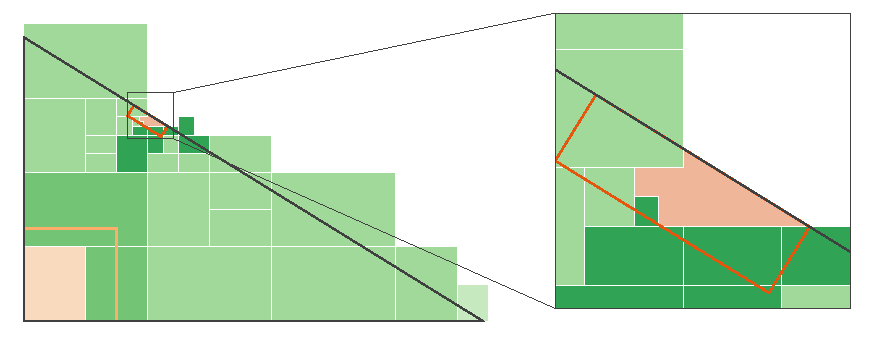
\includegraphics[width=\linewidth]{figures/local-tiling}
\caption{The viewing parameters of the covers around aligned configurations, $s\in[0,2/3]$ horizontally and $t\in[0,2/5]$ vertically, with the viewing triangle outlined: the 30 rows of \cref{tab:local-covers} before enlargement, shaded by their radius (\fc{TileLight}{lightest $1/20$}, then \fc{Sheared}{$1/50$}, \fc{Local}{$1/80$ and $1/96$}, \fc{TileDark}{darkest $1/200$}); \fc{Square}{the square cover's views $[0,1/8]^2$ (light orange)}; and \fc{Pentagon}{the pentagon cover's parallelogram $|\eta|\le1/32$, $-1/32\le\xi\le0$ (red-orange)}. The square and pentagon covers, each a single region, are lightly tinted beneath the rows, which overlap them, and outlined on top. Right: the neighbourhood of the pentagon's viewing parameters, enlarged, where the rows approach the edge-on line in steps.}
\label{fig:local-tiling}
\end{figure}

\begin{table}[ht]
\centering\footnotesize
\setlength{\tabcolsep}{2.2pt}
\begin{tabular}{lllllrrr}
  \toprule
  Cover & Kind & Base; offset & Parameters & Zooms & Cells & Domain & Handed\\
  \midrule
  square & point & $(s,t)$, $\Sigma={[0,1]}^2$; $\mathbf r$ & $\mu_{\max}=\delta_{\max}=\frac18$, $\rho_0=1$ & 18 & 877 & 95 & --\\
  pentagon & point & $(\eta,\xi)$, $\Sigma=[-1,1]{\times}[-1,0]$; $\mathbf r$ & $\mu_{\max}=\frac1{32}$, $\delta_{\max}=\frac1{16}$, $\rho_0=2$ & 24 & 6{,}173 & 0 & --\\
  arc$\pm$ & tube & $e\in[\frac3{64},\frac3{16}]$; $(\frac v2,\theta,\zeta_1,\zeta_3)$ & $\delta_{\max}=\frac1{32}$ & 7 & 343, 288 & 32, 72 & --\\
  endpoint$\pm$ & point & $e-e_*$; $(\frac v2,\theta,\zeta_1,\zeta_3)$ & $\mu_{\max}=\frac1{16},\frac1{32}$, $\delta_{\max}=\frac1{32}$, $\rho_0=1$ & 21 & 305, 246 & 10, 50 & --\\
  crossing$\pm$ & point & $e$; $(\frac{4v}5,\theta,\zeta_1,\zeta_3)$ & $\mu_{\max}=\delta_{\max}=\frac1{16}$, $\rho_0=\frac54$, $\rho_0'=\frac14$ & 28 & 1{,}431, 687 & 31, 160 & 34, 14\\
  \bottomrule
\end{tabular}
\caption{The eight covers of the Exotic component. The offset box is
$\Phi={[-1,1]}^3$ for the square and pentagon and $\Phi=[0,1]\times{[-1,1]}^3$
along the arcs; the pairs are for $\sigma=1$ and $\sigma=-1$, and the
endpoint's two base radii are for $e<e_*$ and $e>e_*$. \emph{Zooms} counts
the zooms of one cover, including the seven sheared zooms of each crossing
cover; \emph{Cells} counts the terminal cells with a witness, and
\emph{Domain} those among them whose witness is an inequality of $D$ (the
fold for $g=k$ at the square, the tie inequality along the arcs).
\emph{Handed} counts the cells handed over by \cref{lem:hand-over}.}
\label{tab:exotic-covers}
\end{table}

\clearpage

\bibliographystyle{plainnat}
\bibliography{references}
\end{document}
